% 152 câu đã gỡ khỏi ngân hàng (chuyen_dang) — chép lại vào file dạng để khôi phục

% từ: cau-hoi/lop10/0D0_Xac_suat/0D0-2-4_Lien_quan_viec_chon_nguoi.tex
\begin{ex}%[0D0H2-4]%[ma:594a93a2]
	Một nhóm có $7$ bạn nam và $6$ bạn nữ. Chọn ngẫu nhiên cùng một lúc ra $5$ bạn đi làm công tác tình nguyện.
	\choiceTF
	{\True Số phần tử của không gian mẫu bằng $1287$}
	{\True Số các kết quả thuận lợi cho biến cố \lq\lq Trong $5$ bạn được chọn có đúng $3$ bạn nam\rq\rq\ bằng là $525$}
	{Số các kết quả thuận lợi cho biến cố \lq\lq Trong $5$ bạn được chọn có ít nhất $3$ bạn nam\rq\rq\ là $231$}
	{\True Số các kết quả thuận lợi cho biến cố \lq\lq Trong $5$ bạn được chọn có nhiều nhất $3$ bạn nam\rq\rq\ là $1056$}
	\loigiai{
		\begin{itemchoice}
			\itemch Đúng. $n\left(\Omega\right)=\mathrm{C}_{13}^5=1287$.
			\itemch Đúng. Chọn $3$ bạn nam có $\mathrm{C}_7^3$.\\
			Chọn $2$ bạn nữ có $\mathrm{C}_6^2$.\\
			Theo quy tắc nhân, có $\mathrm{C}_7^3\cdot \mathrm{C}_6^2=525$ cách chọn $5$ bạn mà có đúng $3$ bạn nam.
			\itemch Sai. Ta có các trường hợp sau:\\
			Chọn $3$ bạn nam, $2$ bạn nữ có $\mathrm{C}_7^3\cdot \mathrm{C}_6^2$ cách.\\
			Chọn $4$ bạn nam, $1$ bạn nữ có $\mathrm{C}_7^4\cdot \mathrm{C}_6^1$ cách.\\
			Chọn $5$ bạn nam có $\mathrm{C}_7^5$ cách.\\
			Theo quy tắc cộng, có $\mathrm{C}_7^3\cdot \mathrm{C}_6^2+\mathrm{C}_7^4\cdot \mathrm{C}_6^1+\mathrm{C}_7^5=756$ cách chọn 5 bạn mà có ít nhất $3$ bạn nam.
			\itemch Đúng. Ta có các trường hợp sau:\\
			Chọn $3$ bạn nam, $2$ bạn nữ có $\mathrm{C}_7^3\cdot \mathrm{C}_6^2$ cách.\\
			Chọn $2$ bạn nam, $3$ bạn nữ có $\mathrm{C}_7^2\cdot \mathrm{C}_6^3$ cách.\\
			Chọn $1$ bạn nam, $4$ bạn nữ có $\mathrm{C}_7^1\cdot \mathrm{C}_6^4$ cách.\\
			Chọn $5$ bạn nữ có $\mathrm{C}_6^5$ cách.\\
			Theo quy tắc cộng, có $\mathrm{C}_7^3\cdot \mathrm{C}_6^2+\mathrm{C}_7^2\cdot \mathrm{C}_6^3+\mathrm{C}_7^1\cdot \mathrm{C}_6^4+\mathrm{C}_6^5=1056$ cách chọn $5$ bạn mà có nhiều nhất $3$ bạn nam.
		\end{itemchoice}
	}
\end{ex}

% từ: cau-hoi/lop10/0D1_Menh_de_Tap_hop/0D1-1-1_Xac_dinh_menh_de_menh_de_chua_bien.tex
\begin{bt}%[0D1B1-1]%[ma:92d7156e]
	Tìm hai giá trị thực của $x$ để từ mỗi câu sau ta được một mệnh  đề đúng và một mệnh đề sai.
	\begin{multicols}{4}
		\begin{enumerate}[a.]
			 \item $x^2<x$.
			\item $x=5x$. 
			\item  $x^2>0$.
			\item $x>\dfrac{1}{x}$. 
		\end{enumerate}
	\end{multicols}
	 \loigiai{
		\begin{enumerate}[a.]
			\item Với  $x=\dfrac{1}{2}$ thì $\left(\dfrac{1}{2}\right)^2<\dfrac{1}{2}$ là mệnh đề đúng. Với $x=1$ thì $1^2<1$ là mệnh đề sai.
			\item Với $x=0$ thì $0=0\cdot 5$ là mệnh đề đúng. Với  $x=-1$ thì $-1=-1\cdot 5$ là mệnh đề sai.
			\item Với $x=3$ thì  $3^2>0$ là mệnh đề đúng. Với $x=0$ thì $0^2>0$ là mệnh đề sai.
			\item Với $x=2$ thì $2>\dfrac{1}{2}$ là mệnh đề đúng. Với $x=-1$ thì $-1>\dfrac{1}{-3}$ là mệnh đề sai. 
		\end{enumerate}
	 }
\end{bt}

% từ: cau-hoi/lop10/0D1_Menh_de_Tap_hop/0D1-1-2_Tinh_dung_sai_cua_menh_de.tex
\begin{ex}%[0D1H1-2]%[ma:0672b2d1]
	Cho  tam giác $ABC$ đều cạnh $2a$. Gọi $M$ là trung điểm $BC$. Khi đó $\left|\overrightarrow{AM}\right|$ bằng
	\choice 
		 {$2a$}
		{$2a\sqrt 3 $} 
		{$4a$} 
		{\True $a\sqrt 3  $}
	 \loigiai{
	\immini 
		{Xét tam  giác $ABM$ vuông tại $M$, ta có\\ $\left|\overrightarrow{AM}\right|=AM=\sqrt{A{B^2}-B{M^2}}\\
		 =\sqrt{(2a)^2-a^2}\\
		 =a\sqrt 3$.}
		{ 
		\begin{tikzpicture}[scale=1,line join=round,line cap=round,font=\footnotesize,>=stealth]
				\def\a{3} 
				\path  (0:0) coordinate (B)
					++(0:\a)  coordinate (C)
					 ([turn]120:\a) coordinate (A)
					 ($(B)!0.5!(C)$) coordinate (M);
				\draw  (A)--(B)--(C)--cycle;
				\foreach \x/  \goc in {A/135,B/-135,C/-45,M/-90}
				 \fill (\x) circle (1pt)
					($(\x)+(\goc:3mm)$) node {$\x$}; 
			\end{tikzpicture}
		} 
	 }
\end{ex}

% từ: cau-hoi/lop10/0D1_Menh_de_Tap_hop/0D1-2-3_Ky_hieu_khoang_doan_nua_khoang.tex
\begin{ex}%[0D1H2-3]%[ma:7a8b9c0d]
% nguon: AI tự sinh (Ôn thi HK)
	Cho các tập hợp số thực $A=(-3;5]$ và $B=[2;7)$.
	\choiceTF
		{\True $A\cap B=[2;5]$}
		{$A\cup B=(-3;7]$}
		{\True $A\setminus B=(-3;2)$}
		{\True $B\setminus A=(5;7)$}
	\loigiai{
		\begin{itemchoice}
			\itemch Đúng. Giao hai tập: từ $2$ đến $5$, lấy cả hai đầu (vì $2\in B$, $5\in A$).
			\itemch Sai. Hợp là $(-3;7)$, không lấy $7$ vì $7\notin B$.
			\itemch Đúng. Loại $[2;5]$ khỏi $(-3;5]$ còn $(-3;2)$.
			\itemch Đúng. Loại $[2;5]$ khỏi $[2;7)$ còn $(5;7)$.
		\end{itemchoice}
	}
\end{ex}

% từ: cau-hoi/lop10/0D3_Ham_so_bac_hai_va_do_thi/0D3-1-1_Xac_dinh_mot_ham_so.tex
\begin{ex}%[0D3V1-1]%[ma:56a4ab5b]
	Cho phương trình đường thẳng $y=ax+b$ có đồ thị đi qua điểm $E(2;-1)$ và song song với đường thẳng $ON$ với $O$ là gốc tọa độ  và $N(1;3)$. Tính giá trị biểu thức $S=a^2+b^2$.
	\choice 
		 {$S=-4$}
		{$S=-40$} 
		{$S=-58$} 
		{\True $S=58$} 
	\loigiai{ 
		Phương trình đường thẳng $ON$ với $O$ là gốc tọa độ và $N(1;3)$ có dạng  $y=3x$.\\
		 Đường thẳng $y=ax+b$ đi qua điểm $E(2;-1) \Leftrightarrow 2a+b=-1$. \qquad(1)\\
		Đường thẳng $y=ax+b$ song song với đường thẳng $ON \Rightarrow \heva{&a=3\\ &b\ne 0.}$  \qquad(2)\\
		Từ $(1)$ và $(2)$ suy  ra $\heva{&a=3\\ &b=-7.}$\\
	Vậy  $S=a^2+b^2=58$.}
\end{ex}

% từ: cau-hoi/lop10/0D3_Ham_so_bac_hai_va_do_thi/0D3-1-3_Gia_tri_cua_ham_so.tex
\begin{ex}%[0D3N1-3]%[ma:ab6795fb]
	Cho hàm số $y=f(x)=\heva{&\sqrt{x+4}&&\text{ khi } x>1\\&x^2+1&&\text{ khi } -1\leq x\leq  1\\&2x-1&&\text{ khi } x<-1}$. Giá trị $f(0)$ bằng
	\choice 
		{$-2$} 
		{$2$} 
		{$-1$} 
		{\True $1$} 
	 \loigiai{
		Ta  có $f(0)=0^2+1=1$.
	 }
\end{ex}

% từ: cau-hoi/lop10/0D3_Ham_so_bac_hai_va_do_thi/0D3-1-4_Do_thi_cua_ham_so.tex
\begin{ex}%[0D3H1-4]%[ma:e395be2c]
	\immini{Cho hàm số $y=f(x)$ có đồ thị như hình vẽ bên.  Mỗi kết quả dưới đây đúng hay sai?}{
	\begin{tikzpicture}[font=\footnotesize,line join=round,line cap=round,>=stealth,scale=1]
			\draw[->] (-2,0) -- (3,0)  node[below] {$x$};
			\draw[->] (0,-3) -- (0,1.5) node[left] {$y$}; 
			\begin{scope}
				 \clip (-2.5,-2.5) rectangle (3,2);
				\draw[samples=200,domain=-2: 5,smooth,variable=\x] plot  (\x,{-(\x)^2+1*(\x)})
					(-1.2,-2) node[above]  {$(P)$};
			\end{scope}
			\foreach  \x/\y in{0/0,1/0,2/0,0/1}{
				\fill (\x,\y) circle (1.5pt); 
			} 
			\path 
				 node at (0,0)[above left]{$O$}
				node at (1,0)[below left]{$1$} 
				node at (2,0)[below]{$2$} 
				node at  (0,1)[left]{$1$};
		\end{tikzpicture}
	} 
	\choiceTF 
		{\True  $f(x)=0\Leftrightarrow \hoac{&x=0\\&x=1}$}
		 {$f(0)=1$}
		{\True  Hàm số đồng biến trên $\left(-\infty;0\right)$}
		 {$1\le f(x)$, $\forall x\in\mathscr{D}$}
	\loigiai{ 
		\begin{itemchoice}
			 \itemch Đồ thị hàm số $y=f(x)$ cắt trục hoành tại hai điểm có hoành độ $x=0$ và $x=1$.
			\itemch Từ đồ  thị hàm số $y=f(x)$ thì $f(0)=0$.
			\itemch Từ đồ thị của hàm số suy ra hàm  số đồng biến trên $\left(-\infty;0\right)$.
			\itemch Từ đồ thị  ta có $f(x)<1$.
		\end{itemchoice}
	} 
\end{ex}

% từ: cau-hoi/lop10/0D3_Ham_so_bac_hai_va_do_thi/0D3-1-4_Do_thi_cua_ham_so.tex
\begin{bt}%[0D3H1-4]%[Tex hóa SGK CD-CT,T7/22, Đoàn Minh Tân]%[ma:cd8e37d1]
	Trong các đường biểu diễn được cho trong hình dưới đây, chỉ ra trường hợp không phải là đồ thị hàm số và giải thích tại sao.\\
	\begin{enumerate}
		\item 
		\begin{tikzpicture}[scale=0.7, font=\footnotesize, line join=round, line cap=round,>=stealth]
			\def \xmin{-2};
			\def \xmax{4};
			\def \ymin{-2};
			\def \ymax{4};
			\draw[->] (\xmin, 0.) -- (\xmax,0.) node[anchor=north] {$x$};
			\draw[->] (0.,\ymin) -- (0.,\ymax) node[anchor=west] {$y$};
			\clip(\xmin-0.1,\ymin-0.1) rectangle (\xmax+0.1,\ymax+0.1);
			\draw[smooth] plot[domain=-2:3.5] (\x,{0.2*(\x)^4-0.56*(\x)^3-0.82*(\x)^2+1.24*(\x)+2.73});
			
		\end{tikzpicture}
		\item
		\begin{tikzpicture}[scale=0.7, font=\footnotesize, line join=round, line cap=round,>=stealth]
			\def \xmin{-2};
			\def \xmax{4};
			\def \ymin{-2};
			\def \ymax{4};
			\draw[->] (\xmin, 0.) -- (\xmax,0.) node[anchor=north] {$x$};
			\draw[->] (0.,\ymin) -- (0.,\ymax) node[anchor=west] {$y$};
			\clip(\xmin-0.1,\ymin-0.1) rectangle (\xmax+0.1,\ymax+0.1);
			\draw (2,3) .. controls (0,2) and (0,1) .. (3.5,-0.5);
			
		\end{tikzpicture}
		\item
		\begin{tikzpicture}[scale=0.7, font=\footnotesize, line join=round, line cap=round,>=stealth]
			\def \xmin{-2};
			\def \xmax{4};
			\def \ymin{-2};
			\def \ymax{4};
			\draw[->] (\xmin, 0.) -- (\xmax,0.) node[anchor=north] {$x$};
			\draw[->] (0.,\ymin) -- (0.,\ymax) node[anchor=west] {$y$};
			\clip(\xmin-0.1,\ymin-0.1) rectangle (\xmax+0.1,\ymax+0.1);
			\draw (-1,2)--(0.5,2)--(0.5,1.5)--(2,1.5)--(2,1)--(3.5,1);
			
		\end{tikzpicture}
		\item
		\begin{tikzpicture}[scale=0.7, font=\footnotesize, line join=round, line cap=round,>=stealth]
			\def \xmin{-2};
			\def \xmax{4};
			\def \ymin{-2};
			\def \ymax{4};
			\draw[->] (\xmin, 0.) -- (\xmax,0.) node[anchor=north] {$x$};
			\draw[->] (0.,\ymin) -- (0.,\ymax) node[anchor=west] {$y$};
			\clip(\xmin-0.1,\ymin-0.1) rectangle (\xmax+0.1,\ymax+0.1);
			\draw (-1,3)--(1.5,0.5)--(3,2);
			
		\end{tikzpicture}
		
	\end{enumerate}
	\loigiai{
		Hai hình biểu diễn ở hình b và hình c không là hàm số vì ứng với mỗi giá trị $x$ có thể có hai (hoặc nhiều) giá trị $y$.
	}
\end{bt}

% từ: cau-hoi/lop10/0D3_Ham_so_bac_hai_va_do_thi/0D3-1-5_Tinh_dong_bien_nghich_bien.tex
\begin{ex}%[0D3N1-5]%[ma:7ea2f53c]
	\immini[thm]{Hàm số bên nghịch biến trên khoảng nào?}{\begin{tikzpicture}[line cap=round,>=stealth,scale=0.7]
		\tikzset{every node/.style={scale=0.7}} 
		\draw[blue,->] (-3,0)--(3,0) node[below left] {$x$}; 
		\draw[blue,->] (0,-3.5)--(0,1) node[below left]  {$y$};
		\draw (0,0) circle (1pt) node [above  left] {$O$};
		 \draw[dashed](1,0) circle (1pt) node[above] {$1$}--(1,-1/2) circle (1pt)--(0,-1/2) circle (1pt) node[below left] {$-\dfrac{1}{2}$};
		\draw[dashed](-1,0) circle (1pt) node[above] {$-1$}--(-1,-1/2)  circle (1pt)--(0,-1/2);
		\draw[red,samples=200,domain=-2.5:2.5,smooth,variable=\x]  plot (\x,{-1/2*(\x)^2});
	\end{tikzpicture}
	 }
	\choice 
		{\True  $(0;+\infty)$}
		 {$(-1; 1)$}
		 {$(-1;+\infty)$}
		{$(-\infty;0)$} 
	\loigiai{Nhìn vào hình dáng đồ thị ta thấy hàm số  nghịch biến trên khoảng $(0; +\infty)$.
	} 
\end{ex}

% từ: cau-hoi/lop10/0D3_Ham_so_bac_hai_va_do_thi/0D3-1-5_Tinh_dong_bien_nghich_bien.tex
\begin{bt}%[0D3N1-5]%[ma:b84ecd9a]
		Hãy cho biết hàm số $y=2x^2$ đồng biến hay nghịch biến trên mỗi khoảng $\left(-\infty;0 \right)$ và $\left(0;+\infty \right)$?
		\loigiai{
			\immini{Dựa vào đồ thị hàm số $y=f(x)=2x^2$
			\begin{itemize}
				\item Trên khoảng $(-\infty;0)$, đồ thị \lq\lq đi xuống\rq\rq~từ trái sang phải và với $x_1, x_2 \in (-\infty;0), x_1 < x_2$ thì $f\left(x_1\right) > f\left(x_2\right)$. Như vậy, hàm số $y=2x^2$ nghịch biến trên khoảng $\left(-\infty;0 \right)$.
				\item Trên khoảng $(0;+\infty)$, đồ thị \lq\lq đi lên\rq\rq~từ trái sang phải và với $x_3, x_3 \in (0;+\infty), x_3 < x_4$ thì $f\left(x_3\right) < f\left(x_4\right)$. Như vậy, hàm số $y=2x^2$ đồng biến trên khoảng $\left(0;\infty \right)$.
			\end{itemize}
			}{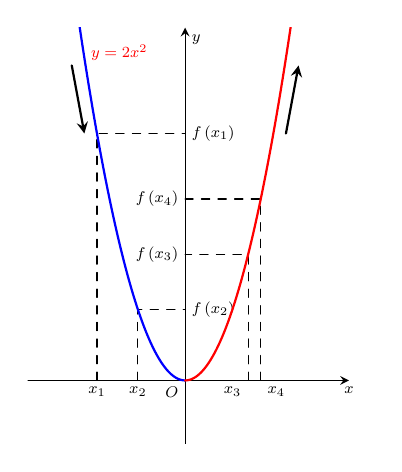
\begin{tikzpicture}[scale=0.8, font=\footnotesize, line join=round, line cap=round, >=stealth]
					\def\a{2}
					\def\b{0}
					\def\c{0}
					\def\f(#1){\a*((#1)^2)+\b*(#1)+\c}
					\def\xmin{-2.5}
					\def\xmax{2.5}
					\def\ymin{-1}
					\def\ymax{4.5}
					\clip (-2.5,5.6) rectangle (3,-1);
					\draw[->] (\xmin-0.1,0)--(\xmax+0.1,0) node[below] { $x$};
					\draw[->] (0,\ymin-0.1)--(0,\ymax+1.1) node[below right] { $y$};
					\draw (0,0) node [below left] { $O$};
					\draw[dashed] (-1.4,0) node[below]{$x_1$}--(-1.4,3.92)--(0,3.92) node[right]{$f\left(x_1\right)$}
					(-0.75,0)node[below]{$x_2$}--(-0.75,1.125)--(0,1.125) node[right]{$f\left(x_2\right)$}
					(1,0)node[below left]{$x_3$}--(1,2)--(0,2) node[left]{$f\left(x_3\right)$}
					(1.2,0)node[below right]{$x_4$}--(1.2,2.88)--(0,2.88) node[left]{$f\left(x_4\right)$};
					\draw[thick,->] (-1.8,5)--(-1.6,3.92);
					\draw[thick,->] (1.6,3.92)--(1.8,5);	
					\draw[blue,thick,smooth,samples=200] plot[domain=\xmin:0] (\x,{\f(\x)});
					\draw[red,thick,smooth,samples=200] plot[domain=0:\xmax] (\x,{\f(\x)});
					\draw (-1.6,5.2) node [red,right, sloped] {$y=2x^2$};
			\end{tikzpicture}}					
		}
	\end{bt}

% từ: cau-hoi/lop10/0D3_Ham_so_bac_hai_va_do_thi/0D3-1-5_Tinh_dong_bien_nghich_bien.tex
\begin{bt}%[0D3H1-5]%[Huỳnh Đức Vũ]%[0D2K1]%[ma:dbd485f8]
	\immini{Cho hàm số $y=f(x)$ xác định trên $(-6;+\infty)$, có đồ thị như hình vẽ bên. Tìm các khoảng đồng biến, các khoảng nghịch biến của hàm số.}{
		\begin{tikzpicture}[>=stealth,line join=round,line cap=round,font=\footnotesize,scale=0.6]			
			\draw[-> ] (-6.5,0) -- (2,0)node[below] {$x$};
			\draw[-> ] (0,-1.0) -- (0,11)node[right] {$y$};
			\draw(0,0) node[below left=-0.05] {$O$};
			\draw[red,smooth,samples=100,domain=-3:1.12]  plot (\x,{(\x)^2+4*(\x)+5});
			\draw[red] (-6,2)--(-3,2);
			\draw[dashed] (-6,0)node[below]{$-6$}--(-6,2) (-3,0)node[below]{$-3$}--(-3,2)--(0,2)node[right]{$2$};
			\draw[dashed](-2,0)node[below]{$-2$}--(-2,1)--(0,1)node[right]{$1$};
			\draw (0,5)node[right]{$5$};
			\draw[dashed](1,0)node[below]{$1$}--(1,10)--(0,10)node[left]{$10$};
			\fill (-6,0) circle(1pt) (-3,0) circle(1pt) (-2,0) circle(1pt) (-6,2) circle(1pt)(-3,2) circle(1pt)
			(-2,1) circle(1pt)
			(1,10) circle(1pt)
			(-2,-1) circle(1pt)(0,1) circle(1pt)(0,2) circle(1pt)
			(0,5) circle(1pt);		
	\end{tikzpicture}}
	\loigiai{Từ đồ thị, ta có hàm số không đổi trên $(-6;-3)$, nghịch biến trên $(-3;-2)$ và đồng biến trên $(-2;+\infty)$.}
\end{bt}

% từ: cau-hoi/lop10/0D3_Ham_so_bac_hai_va_do_thi/0D3-1-5_Tinh_dong_bien_nghich_bien.tex
\begin{bt}%[0D3V1-5]%[Dự án Tex Toán 10 chương trình mới]%[ma:4a9bde19]
	Tìm giá trị thực của tham số $a$ để hàm số $y=\dfrac{ax}{x-2}$ đồng biến trên khoảng $\left(2;+\infty\right)$.
	\loigiai{Ta có $y=\dfrac{ax}{x-2}=a+\dfrac{2a}{x-2}$.\\
		Với mọi $x_1$, $x_2 \in \left(2;+\infty\right)$, $x_1 \neq x_2$, ta có
		\begin{equation*}
			K=\dfrac{f(x_1)-f(x_2)}{x_1-x_2}=\dfrac{\dfrac{2a}{x_1-2}-\dfrac{2a}{x_2-2}}{x_1-x_2}=-\dfrac{2a}{\left(x_1-2\right)\left(x_2-2\right)}.
		\end{equation*}
		Đề hàm số $y=\dfrac{ax}{x-2}$ đồng biến trên khoảng $\left(2;+\infty\right)$ thì $K>0$, $\forall x \in \left(2;+\infty\right)$.\\
		 Mặt khác, $\left(x_1-2\right)\left(x_2-2\right)>0$, với mọi $x_1$, $x_2 \in \left(2;+\infty\right)$, $x_1 \neq x_2$. Do đó
		\begin{equation*}
			K>0, \forall x \in \left(2;+\infty\right) \Leftrightarrow -2a>0 \Leftrightarrow a<0.
		\end{equation*} 
		Vậy $a<0$ thỏa yêu cầu bài toán.}
\end{bt}

% từ: cau-hoi/lop10/0D3_Ham_so_bac_hai_va_do_thi/0D3-1-5_Tinh_dong_bien_nghich_bien.tex
\begin{bt}%[0D3H1-5]%[0K6YE-4]%[ma:4474f4c6]
	\immini
	{Dựa vào đồ thị hàm số $y=\dfrac{1}{2}x^2$ (như hình vẽ), cho biết hàm số $y=\dfrac{1}{2}x^2$ đồng biến hay nghịch biến trên khoảng $(0;+\infty)$ và $(-\infty;0)$.}
	{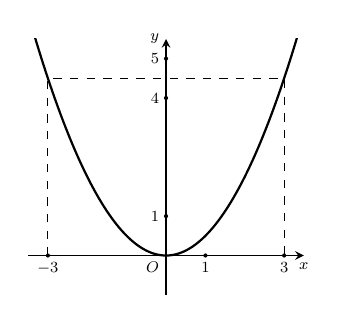
\begin{tikzpicture}[>=stealth,x=1cm,y=1cm,font=\footnotesize,scale=0.5]
			\def\a{1/2}
			\draw[->] (-3.5,0) -- (3.5,0) node[below] {$x$};
			\draw[->] (0,-1) -- (0,5.5) node[left] {$y$};
			\draw (0,0)node[below left]{$O$};
			\fill (-3,0)node[below]{$-3$} circle(1.5pt);
			\fill (1,0)node[below]{$1$} circle(1.5pt);
			\fill (3,0)node[below]{$3$} circle(1.5pt);
			\fill (0,1)node[left]{$1$} circle(1.5pt);
			\fill (0,4)node[left]{$4$} circle(1.5pt);
			\fill (0,5)node[left]{$5$} circle(1.5pt);
			\clip (-3.5,-1)rectangle(3.5,5.5);
			\draw[thick,samples=150,smooth,domain=-3.5:3.5] plot(\x,{\a*(\x)^2});
			\draw[dashed] (-3,0)--(-3,4.5)--(3,4.5)--(3,0);
	\end{tikzpicture}}
	\loigiai{
		Dựa vào đồ thị hàm số $y=\dfrac{1}{2}x^2$ ta có
		\begin{itemize}
			\item Trên khoảng $(-\infty;0)$, đồ thị \lq\lq đi xuống\rq\rq\, từ trái sang phải và với $x_1; x_2\in(-\infty;0),\,\,x_1<x_2$ thì $f\left(x_1\right)>f\left(x_2\right)$. Như vậy, hàm số $y=\dfrac{1}{2}x^2$ nghịch biến trên khoảng $(-\infty;0)$.
			\item Trên khoảng $(0;+\infty)$, đồ thị \lq\lq đi lên\rq\rq\, từ trái sang phải và với $x_1; x_2\in(0;+\infty),\,\,x_1<x_2$ thì $f\left(x_1\right)<f\left(x_2\right)$. Như vậy, hàm số $y=\dfrac{1}{2}x^2$ đồng biến trên khoảng $(0;+\infty)$.
		\end{itemize}       
	}
\end{bt}

% từ: cau-hoi/lop10/0D3_Ham_so_bac_hai_va_do_thi/0D3-2-1_Xac_dinh_ham_so_bac_hai.tex
\begin{ex}%[0D3B2-1]%[ma:c3d832cd]
	Gieo một đồng tiền liên tiếp $3$ lần. Xác suất của biến cố $A$: “Kết  quả của $3$ lần gieo là như nhau” là
	 \choice
		{$\dfrac{1}{2}$} 
		 {$\dfrac{3}{8}$}
		{$\dfrac{7}{8}$} 
		{\True  $\dfrac{1}{4}$}
	 \loigiai{
		Ta  có $n(\Omega)=8$.\\
		Biến cố $A$ \lq\lq Kết quả của $3$ lần gieo là như nhau\rq\rq.\\ 
		$A=\left\{NNN,SSS\right\}$,  suy ra $n(A)=2$.\\
		Vậy xác suất biến cố $A$ là $\mathrm{P}(A)=\dfrac{n(A)}{n(\Omega)}=\dfrac{2}{8}=\dfrac{1}{4}$. 
	 }
\end{ex}

% từ: cau-hoi/lop10/0D3_Ham_so_bac_hai_va_do_thi/0D3-2-2_Bang_bien_thien_tinh_don_dieu_max_min.tex
\begin{ex}%[0D3H2-2]%[ma:a52b47fa]
	 Cho hàm số $y =-x^2+6x+2$. Các khẳng định sau đây đúng hay sai?
	 \choiceTF
		{Hàm số đạt giá trị nhỏ nhất bằng  $-11$}
		{\True Hàm số đồng biến trên $(-\infty;3)$} 
		{\True Hàm số đạt giá trị lớn  nhất bằng $11$}
		{Hàm số nghịch biến  trên $(0;+\infty)$}
	\loigiai{ 
		\begin{itemchoice}
			\itemch  Hàm số đạt giá trị lớn nhất bằng $11$ tại $x=3$.
			 \itemch Hàm số đồng biến trên $(-\infty;3)$.
			\itemch Hàm số nghịch biến trên  $(3;+\infty)$.
		\end{itemchoice}
	 }
\end{ex}

% từ: cau-hoi/lop10/0D3_Ham_so_bac_hai_va_do_thi/0D3-2-2_Bang_bien_thien_tinh_don_dieu_max_min.tex
\begin{ex}%[0D3H2-2]%[ma:357a30a0]
	Cho hàm số bậc hai có  bảng biến thiên
	\begin{center}
		
\begin{tikzpicture}
				 \tkzTabInit[lgt=1.5,espcl=2.5,deltacl=.5]
					{$x$ /.7,$y$  /2}
					{$+\infty$,$-1$,$+\infty$} 
				 \tkzTabVar{+/$+\infty$,-/ $2$,+/$+\infty$}
			\end{tikzpicture}
	\end{center}
	Các khẳng định sau đây  đúng hay sai?
	 \choiceTF
		{\True Hàm số đồng biến trên $(-1;+\infty)$} 
		{\True Hàm số đạt giá trị nhỏ  nhất bằng $2$}
		{Hàm  số nghịch biến trên $(-\infty;2)$}
		{Hàm  số đạt giá trị nhỏ nhất tại $x=2$}
	\loigiai{ 
		\begin{itemchoice}
			\itemch Hàm số đồng  biến trên $(-1;+\infty)$.
			\itemch Hàm số nghịch  biến trên $(-\infty;-1)$.
			\itemch Hàm số đạt giá trị nhỏ nhất  bằng $2$ tại $x=-1$.
		\end{itemchoice}
	 }
\end{ex}

% từ: cau-hoi/lop10/0D3_Ham_so_bac_hai_va_do_thi/0D3-2-3_Do_thi_cua_ham_so_bac_hai.tex
\begin{ex}%[0D3B2-3]%[ma:a06138fc]
	Tìm một đội gồm $ 5 $ nam và $ 8 $ nữ. Lập một nhóm  gồm $ 4 $ người hát tốp ca, tính xác suất để trong $ 4 $ người được chọn có ít nhất $ 3 $ nữ.
	 \choice
		 {$\dfrac{56}{143}$}
		{$\dfrac{87}{143}$} 
		 {\True $\dfrac{70}{143}$}
		{$\dfrac{73}{143}$} 
	\loigiai{ 
		Số phần tử của không gian mẫu  $ \mathrm{C}^4_{13}=715 $.\\
		Số  cách chọn $ 4 $ người có ít nhất $ 3 $ nữ là $ \mathrm{C}^3_8\cdot \mathrm{C}^1_5+\mathrm{C}^4_8=350$.\\
		Vậy xác suất cần tìm là  $ P=\dfrac{70}{143} $.
	} 
\end{ex}

% từ: cau-hoi/lop10/0D3_Ham_so_bac_hai_va_do_thi/0D3-2-3_Do_thi_cua_ham_so_bac_hai.tex
\begin{ex}%[0D3B2-3]%[ma:8072c2d8]
	Lớp A có $9$ học sinh xuất sắc, lớp B có $10$ học sinh xuất  sắc. Chọn ngẫu nhiên $2$ trong các học sinh
	đó đi dự lễ tuyên dương học sinh tiêu biểu. Xác suất để $2$ học sinh được chọn từ cùng một  lớp là?
	 \choice
		{$\dfrac{10}{19}$} 
		{\True  $\dfrac{9}{19}$}
		{$\dfrac{13}{18}$} 
		 {$\dfrac{11}{18}$}
	\loigiai{ 
		Ta  có $n(\Omega)=\mathrm{C}_{19}^2=171$.\\
		Biến  cố $A$ \lq\lq$2$ học sinh được chọn từ cùng một lớp\rq\rq.\\
		 Suy ra, $n(A)=\mathrm{C}_{10}^2+\mathrm{C}_9^2=81$.\\
		Vậy xác suất biến cố  $A$ là $\mathrm{P}(A)=\dfrac{n(A)}{n(\Omega)}=\dfrac{81}{171}=\dfrac{9}{19}$.
	 }
\end{ex}

% từ: cau-hoi/lop10/0D3_Ham_so_bac_hai_va_do_thi/0D3-2-6_Toan_thuc_te_ung_dung_ham_so_bac_hai.tex
\begin{bt}%[0D3H2-6]%[6.13 sách kết nối]%[ma:7171f09a]
	Bác Hùng dùng 40 m lưới thép gai rào thành một mảnh vườn hình chữ nhật để trồng rau.
	\begin{enumerate}
		\item Tính diện tích mảnh vườn hình chữ nhật rào được theo chiều rộng $x$ (mét) của nó.
		\item Tìm kích thước của mảnh vườn hình chữ nhật có diện tích lớn nhất mà bác Hùng có thể rào được.
	\end{enumerate}
	\loigiai{
		\begin{enumerate}
			\item Gọi $y$ (mét) là chiều rộng của hình chữ nhật. Điều kiện $x,y>0$.\\
			Vì bác Hùng dùng 40 m lưới thép gai rào thành một mảnh vườn hình chữ nhật để trồng rau nên chu vi của hình chữ nhật là 40 m suy ra $2\left(x+y\right)=40\Rightarrow x+y=20\Rightarrow y=20-x.$\\
			Diện tích mảnh vườn hình chữ nhật là $S=xy=x\left(20-x\right)=-x^2+20x.$
			\item Vì $y>0$ nên $20-x>0\Rightarrow 0<x<20$.\\
			Hàm số $S\left(x\right)=-x^2+20x$ có bảng biến thiên
			\begin{center}
				
\begin{tikzpicture}
					\tkzTabInit[nocadre=true,lgt=1.2,espcl=2.5,deltacl=0.6]
					{$x$ /0.6,$S\left(x\right)$ /2}
					{$0$,$10$,$20$}
					\tkzTabVar{-/$0$, +/$100$,-/$0$}
				\end{tikzpicture}
			\end{center}
			Dựa vào bảng biến thiên ta thấy diện tích lớn nhất mà bác Hùng có thể rào được là 100 $\text{m}^2$ khi mảnh vườn có hình vuông cạnh 10 m.
	\end{enumerate}}
\end{bt}

% từ: cau-hoi/lop10/0D3_Ham_so_bac_hai_va_do_thi/0D3-2-6_Toan_thuc_te_ung_dung_ham_so_bac_hai.tex
\begin{bt}%[0D3V2-6]%[GHKII-2022-2023-TRƯỜNG THPT NGUYỄN HỮU HUÂN-Thehung Nguyen]%[ma:25fcd7e8]
	Một đoạn kẽm dài $6$ mét được cắt ra làm hai phần: một phần uốn thành hình vuông có cạnh bằng $x$ mét, phần còn lại uốn thành hình chữ nhật có chiều dài gấp $3$ lần chiều rộng. Tìm điều kiện của $x$ để diện tích hình chữ nhật lớn hơn diện tích hình vuông (Làm tròn kết quả đến hàng phần chục).
	\loigiai{
		Đoạn kẽm uốn thành hình vuông có cạnh là $x$ (m) nên đoạn kẽm đó là $4x$ (m).\\
		 Điều kiện $0<x<\dfrac{3}{2}$.\\
		 Diện tích hình vuông là $x^2$.\\
		 Gọi $y$ (m) là chiều rộng hình chữ nhật, suy ra $2(y+3y)=6-4x$ hay $y=\dfrac{3}{4}-\dfrac{1}{2}x$.\\
		 Diện tích hình chữ nhật là $3y\cdot y=3\cdot\left(\dfrac{3}{4}-\dfrac{1}{2}x\right)^2$.\\
		 Theo đề bài ta có bất phương trình
		 \allowdisplaybreaks
		 \begin{eqnarray*}
		 	&&3\cdot\left(\dfrac{3}{4}-\dfrac{1}{2}x\right)^2>x^2\\
		 	&\Leftrightarrow&\dfrac{27}{16}-\dfrac{9}{4}x+\dfrac{3}{4}x^2>x^2\\
		 	&\Leftrightarrow&4x^2+36x-27<0\\
		 	&\Leftrightarrow&-9{,}696\approx\dfrac{-9-6\sqrt{3}}{2}<x<\dfrac{-9+6\sqrt{3}}{2}\approx 0{,}696.
		 \end{eqnarray*}
		Kết hợp với điều kiện $0<x<0{,}7$ (đơn vị của $x$ là mét) thỏa yêu cầu bài toán.
	}
\end{bt}

% từ: cau-hoi/lop10/0D3_Ham_so_bac_hai_va_do_thi/0D3-2-6_Toan_thuc_te_ung_dung_ham_so_bac_hai.tex
\begin{bt}%[0D3H2-6]%[Đề GHKII 2022-2023, TheHung Nguyen]%[Thpt Nguyễn Hữu Cảnh]%[ma:046119a4]
	Anh An dùng $60$ m lưới rào quanh một mảnh vườn hình chữ nhật đề trồng rau. Biết rằng một cạnh theo chiều dài vườn là một bức tường (nên không cần rào), do đó anh An chi cần rào ba cạnh còn lại của hình chữ nhật để làm vườn. Giả sử diện tích mành vườn không nhỏ hơn $400$m$^2$. Hỏi chiều rộng của mảnh vườn có giá trị nhỏ nhất là bao nhiêu?
	\loigiai{Gọi $x$ là chiều rộng của mảnh vườn hình chữ nhật, (đơn vị là mét). Điều kiện $x>0$.\\
		Khi đó chiều dài phải rào của khu vườn là $60-2x$. \\
		Vì diện tích khu vườn không nhỏ hơn $400$ m$^2$ nên ta có
		$$x(60-2x)\ge 400\Leftrightarrow -2x^2+60x-400\ge 0\Leftrightarrow 10\le x\le 20.$$
		Vậy chiều rộng của vườn cần có giá trị nhỏ nhất là $10$ m.
	}
\end{bt}

% từ: cau-hoi/lop10/0D7_Bat_phuong_trinh_bac_2_mot_an/0D7-1-2_Dau_cua_tam_thuc_bac_2_va_ung_dung.tex
\begin{bt}%[0D7V1-2]%[ma:22aeb5d5]
	Biết  $\left[\dfrac{a}{b}; c\right]$ là tập hợp tất cả các giá trị của tham số $m$ để bất phương trình $(m-1)x^2 - 2(m-2)x + 2 - m < 0$ vô nghiệm. Tìm giá trị của biểu thức $M=\dfrac{a c}{b}$.
	\loigiai{ 
		Giả sử bất phương trình  $(m-1)x^2 - 2(m-2)x + 2 - m < 0$ vô nghiệm. \\
		Suy ra $(m-1)x^2 -  2(m-2)x + 2 - m \geq 0$, $\forall x \in \mathbb{R}$. \\
		Ta xét hai trường hợp $m-1=0$ hoặc $m-1>0$ vì trường hợp $m-1<0$  không xảy ra.\\
		Xét $m-1=0$, ta được 
		$\heva{& m-1 = 0 \\& -2(m-2) = 0 \\& 2 -  m \geq 0}
		\Leftrightarrow  \heva{& m = 1 \\ & m = 2 \\ & m \leq 2.}$ (vô lý). \\
		Xét  $m-1>0$, ta được
		$\heva{ & m-1 > 0 \\ & \Delta = (m-2)^2  - (m-1)(2-m) \leq 0} \Leftrightarrow
		\heva{ & m  > 1\\ & 2m^2 - 7m + 6 \leq 0}
		\Leftrightarrow 
		\dfrac{3}{2} \leq m \leq 2 
		$.  \\
		Suy ra tập hợp tất cả các giá trị của tham số  $m$ thỏa yêu cầu là $\left[\dfrac{3}{2}; 2\right]$.\\
		Do đó, $a =  3$, $b = 2$, $c = 2$. \\
		Vậy $M  = \dfrac{a c}{b} = \dfrac{3 \cdot 2}{2} = 3$.
	} 
\end{bt}

% từ: cau-hoi/lop10/0D7_Bat_phuong_trinh_bac_2_mot_an/0D7-1-4_Xet_dau_bieu_thuc_dang_tich_thuong.tex
\begin{ex}%[0D7H1-4]%[ma:eb915c30]
	Tập nghiệm bất phương trình $\left(9-x^{2}\right)(2x-10)<0$  là
	\choice 
		{$(-\infty;-3)\cup(3;5)$} 
		{$(-\infty;-3)\cup(5;+\infty)$} 
		 {$(-3;3)$}
		{\True  $(-3;3)\cup(5;+\infty)$}
	\loigiai{ 
		 Xét $\left(9-x^{2}\right)(2x-10)=0\Leftrightarrow\hoac{&x=\pm 3\\&x=5.}$\\
		 Bản xét dấu
		\begin{center}
			
\begin{tikzpicture}
					\tkzTabInit[nocadre=true,lgt=3,espcl=2,deltacl=0.5] 
						{$x$/0.7,$9-x^2$/0.7,$2x-10$/.7,$(9-x^2) 
						 (2x-10)$/.7}
						{$-\infty$,$-3$,$3$,$5$,$+\infty$} 
					\tkzTabLine{,-,$0$,+,$0$,-,|,-,} 
					 \tkzTabLine{,-,|,-,|,-,$0$,+,}
					 \tkzTabLine{,+,$0$,-,$0$,+,$0$,-,}
				\end{tikzpicture}
		\end{center}
		Dựa  vào bảng xét dấu, suy ra $\left(9-x^{2}\right)(2x-10)<0$ khi $x\in(-3;3)\cup(5;+\infty)$.\\
		Vậy tập nhiệm của  bất phương trình $\left(9-x^{2}\right)(2x-10)<0$ là $(-3;3)\cup(5;+\infty)$.
	 }
\end{ex}

% từ: cau-hoi/lop10/0D7_Bat_phuong_trinh_bac_2_mot_an/0D7-2-1_Bat_phuong_trinh_bac_2_va_ung_dung.tex
\begin{ex}%[0D7H2-1]%[ma:c1e84d7d]
	Cho tam thức bậc hai $f(x)=x^2+mx+n$, $(m, \,n \in  \mathbb{R})$ có $\Delta<0$. Khẳng định nào sau đây đúng?
	 \choice
		{$f(x)=0 \Leftrightarrow  x=-\dfrac{m}{2}$}
		 {$f(x)<0, \forall x \in(0;+\infty)$}
		 {\True $f(x)>0, \forall x \in \mathbb{R}$}
		 {$f(x)<0, \forall x \in \mathbb{R}$}
	 \loigiai{
		Tam  thức bậc hai $f(x)=x^2+mx+n$, $(m, \,n \in \mathbb{R})$ có $a=1>0$, $\Delta<0$.\\
		Vậy $f(x)>0, \forall x \in \mathbb{R}$. 
	 }
\end{ex}

% từ: cau-hoi/lop10/0D7_Bat_phuong_trinh_bac_2_mot_an/0D7-2-3_Bat_phuong_trinh_dang_tich_thuong.tex
\begin{bt}%[0D7V2-3]%[Dự án đề kiểm tra HKII NH22-23- BCTuan]%[THPT Võ Văn Kiệt TPHCM]%[ma:ccfa0cee]
\begin{enumerate}
	\item Giải bất phương trình $(x-4)(x^2+5x-6)\ge 0$.
	\item Giải phương trình $\sqrt{2x^2-9x-4}=\sqrt{x^2-3x-4}$.
	\item Giải phương trình $\sqrt{3x^2+6x+7}+\sqrt{5x^2+10x+14}=4-2x-x^2$.
\end{enumerate}
\loigiai{
\begin{enumerate}
	\item Ta có
	\begin{eqnarray*}
	&&	(x-4)(x^2+5x-6)\ge 0\\
	&\Leftrightarrow &\hoac{&\heva{& x-4\ge 0 \\ & x^2+5x-6\ge 0}\\&\heva{& x-4\le 0 \\ & x^2+5x-6\le 0}} \Leftrightarrow \hoac{& \heva{& x\ge 4 \\ & \hoac{& x\ge 1 \\ & x\le -6}} \\ & \heva{& x\le 4 \\ & -6\le x\le 1}}\\
	&\Leftrightarrow & \hoac{& x\ge 4 \\ & -6\le x\le 1.}
	\end{eqnarray*}
Vậy tập nghiệm của bất phương trình là $S=[-6;1]\cup [4;+\infty)$.
\item Ta có
\begin{eqnarray*}
&&\sqrt{2x^2-9x-4}=\sqrt{x^2-3x-4}\\
&\Rightarrow & 2x^2-9x-4=x^2-3x-4\\
&\Leftrightarrow & x^2-6x=0\Leftrightarrow \hoac{& x=0 \\ & x=6.}
\end{eqnarray*}
Thay các nghiệm $x=0$, $x=6$ vào phương trình ban đầu ta thấy chỉ có nghiệm $x=6$ thỏa mãn.\\
Vậy tập nghiệm của phương trình là $S=\{6\}$.
\item Ta có 
\begin{itemize}
	\item $\sqrt{3x^2+6x+7}=\sqrt{3(x+1)^2+4}\ge 2$,\ $\forall x\in\mathbb{R}$.
	\item $\sqrt{5x^2+10x+14}=\sqrt{5(x+1)^2+9}\ge 3$,\ $\forall x\in\mathbb{R}$.
	\item $4-2x-x^2=5-(x+1)^2\le 5$,\ $\forall x\in\mathbb{R}$.
\end{itemize}
Vậy $\sqrt{3x^2+6x+7}+\sqrt{5x^2+10x+14}\ge 5\ge 4-2x-x^2$,\ $\forall x\in\mathbb{R}$.\\
Vậy phương trình đã cho tương đương $$\heva{& \sqrt{3x^2+6x+7}+\sqrt{5x^2+10x+14}=5 \\ & 4-2x-x^2=5}\Leftrightarrow x=-1.$$
Vậy tập nghiệm của phương trình là $S=\{-1\}$.
\end{enumerate}
}
\end{bt}

% từ: cau-hoi/lop10/0D7_Bat_phuong_trinh_bac_2_mot_an/0D7-2-6_Bai_toan_co_tham_so.tex
\begin{bt}%[Bài Giảng K10-K11, Đỗ Viết Lân]%[0D7V2-6]%[ma:09b20ccd]
	Tìm các giá trị của tham số $m$ để tam thức bậc hai $-x^2+2\left(2m-3\right)x-4m+3<0 ,\,\forall x \in \mathbb{R}$.
	\loigiai{
		\allowdisplaybreaks
		\begin{eqnarray*}
			&&-x^2+2\left(2m-3\right)x-4m+3<0,\,\forall x \in \mathbb{R}\\
			&\Leftrightarrow& \heva{& -1<0\\& \left[2(2m-3)\right]^2-4\cdot (-1)\cdot (-4m+3)< 0}\\
			&\Leftrightarrow& 16m^2- 64m +48 <0\\
			&\Leftrightarrow & 1<m<3.
		\end{eqnarray*}
	}
\end{bt}

% từ: cau-hoi/lop10/0D7_Bat_phuong_trinh_bac_2_mot_an/0D7-2-7_Toan_thuc_te_ung_dung_bat_phuong_trinh_bac_2.tex
\begin{bt}%[0D7V2-7]%[ma:cc9ed517]
	Bác Hùng dùng $40$ m lưới thép gai rào thành một mảnh vườn hình chữ nhật để trồng rau. Gọi $x$  (m) là kích thước chiều rộng của hình chữ nhật. Để diện tích mảnh vườn nói trên không nhỏ hơn $91$ m$^2$ thì $x\in [a;b]$. Tính $b-a$.
	 \shortans{3}
	\loigiai{ 
		 Diều kiện $0<x\leq 10$.\\
		Để diện tích mảnh vườn  lớn hơn 91 m$^2$ thì $x(20-x)\geq 91\Leftrightarrow -x^2+20x-91\geq 0$.\\
		Suy  ra $x\in [7;13]$ mà $x$ là chiều rộng nên $x\in [7;10]$.\\
		Vậy  $b-a=10-7=3$.
	 }
\end{bt}

% từ: cau-hoi/lop10/0D7_Bat_phuong_trinh_bac_2_mot_an/0D7-3-5_Phuong_trinh_khac_quy_ve_phuong_trinh_bac_2.tex
\begin{ex}%[0D7H3-5]%[ma:30984551]
	Cho phương trình $x^{2}-2x+m-5=0$ có hai nghiệm phân biệt $x_{1}$, $x_{2}$ thỏa mãn $x_{1}\cdot x_{2}=-8$. Phương trình có số nghiệm nguyên âm là 
	\choice 
		{$2$} 
		 {$0$}
		{\True $1$} 
		 {$3$}
	 \loigiai{
		Phương trình có hai nghiệm  phân biệt $x_{1}$, $x_{2}$ thỏa mãn $x_{1}\cdot x_{2}=-8$.\\
		 Ta có $\heva{&\Delta'>0\\&x_1\cdot x_{2}=-8}\Leftrightarrow\heva{&-m+6>0\\&m-5=-8}\Leftrightarrow\heva{&m<6\\&m=-3}\Leftrightarrow m=-3$.\\
		Khi đó ta  có phương trình $x^{2}-2x-8=0\Leftrightarrow\hoac{&x=4\\&x=-2.}$\\
		Vậy phương  trình có $1$ nghiệm nguyên âm.
	 }
\end{ex}

% từ: cau-hoi/lop10/0D7_Bat_phuong_trinh_bac_2_mot_an/0D7-3-6_Toan_hinh_toan_thuc_te_ung_dung_phuong_trinh.tex
\begin{ex}%[0D7V3-6]%[Dự án Bài Giảng 10-11 Nhóm Toán & LaTex, Nguyễn Anh Tuấn]%[ma:bcab6be6]
	\immini{
		Một con tàu biển $M$ rời cảng $O$ và chuyển động thẳng theo phương tạo với bờ biển một góc $60^{\circ}$. Trên bờ biển có hai đài quan sát $A$ và $B$ nằm về hai phía so với cảng $O$ và lần lượt cách cảng $O$ khoảng cách $1$ km và $2$ km (hình bên).  Khoảng cách từ tàu đến $B$ bằng $\dfrac{4}{5}$ khoảng cách từ tàu đến $A$. Đặt độ dài của $MO$ là $x \mathrm{~km}$.
	}{
		\begin{tikzpicture}[scale=1, line cap=round, line join=round,font=\footnotesize, >=stealth]
			\def\a{1}
			\path 	(0:0) coordinate (O)
			++(0:2*\a) coordinate (B)
			++(180:3*\a) coordinate (A)
			($(O)!1.2!60:(B)$) coordinate (M);
			\draw[thick] (A)--(B)--(M)--cycle (O)--node[rotate=60, yshift=-1.5mm, scale=.7]{$x \mathrm{~km}$}(M);
			\foreach \i in {-1,-.9,...,2.1}{
				\draw (\i,0)--(\i-.1,-.1);
			}
			\foreach \x/\g in {A/200,B/-20,O/-90,M/90}
			\fill[black] (\x) circle (1pt)
			($(\g:3mm)+(\x)$) node[scale=.8] {$\x$};
			\draw (O) node[shift={(0.4,0.2)},scale=0.7]{$60^{\circ}$};
		\end{tikzpicture}
	}
	\choiceTF
	{Khoảng cách giữa $A$ và $M$ là $AM=\sqrt{x^2+x-1}$ km}
	{\True Khoảng cách giữa $B$ và $M$ là $BM=\sqrt{x^2-2x+4}$ km}
	{Khoảng cách giữa hai đài quan sát là $4$ km}
	{\True Biết rằng $x>2$. Khoảng cách giữa $M$ và $O$ là $x=5{,}69$ km}
	\loigiai{
		
		\begin{itemchoice}
			\itemch Áp dụng định lí hàm số cosin trong tam giác $AMO$, ta được 
			\[AM^2=OM^2+OA^2-2OM\cdot OA\cos \left(180^\circ-60^\circ\right)
			=x^2+1+x \Rightarrow AM=\sqrt{x^2+x+1}.\]
			\itemch Áp dụng định lí hàm số cosin trong tam giác $BMO$, ta được
			\[BM^2=OM^2+OB^2-2OM\cdot OB\cos 60^\circ
			=x^2+4-2x \Rightarrow BM=\sqrt{x^2-2x+4}.\]
			\itemch Ta có $AB=AO+OB=1+2=3$ km.
			\itemch Theo giả thiết, ta có
			\begin{eqnarray*}
				BM=\dfrac{4}{5}AM 
				&\Leftrightarrow& \sqrt{x^2-2x+4}=\dfrac{4}{5}\sqrt{x^2+x+1} \\
				&\Leftrightarrow&  25\left(x^2-2x+4\right)=16\left(x^2+x+1\right) \\
				&\Leftrightarrow& 9x^2-66x+84=0 \\
				&\Leftrightarrow& \hoac{&x \approx 5{,}69\\
					&x\approx 1{,}64.}
			\end{eqnarray*}
			Vì $x>2$ nên $x=5{,}69$ km.
		\end{itemchoice}
	}
\end{ex}

% từ: cau-hoi/lop10/0H4_He_thuc_luong_trong_tam_giac/0H4-2-1_Bai_toan_chi_dung_dinh_ly_Sin_Cosin.tex
\begin{bt}%[0H4H2-1]%[ma:66e4858f]
	Hình bình hành có hai cạnh là $5$ và $9$, một đường chéo bằng $11$.  Tìm độ dài đường chéo còn lại
	\loigiai{ 
		\begin{center}
			\begin{tikzpicture}[>=stealth,line join=round,line cap=round]
					\draw  (0,0) coordinate (A)--(0:4) coordinate (B)--($(80:2)+(0:4)$) coordinate (C)--(80:2) coordinate (D)--cycle;
					\foreach \diem/\vitrin in {A/left,B/right,C/right,D/left} \fill[black](\diem)  circle (1.5pt) node[\vitrin]{$\diem$};
					\path (A)--(B)  node[pos=0.5,sloped,below]{$9$};
					\path  (A)--(D) node[pos=0.5,left]{$5$};
					 \path (D)--(B) node[pos=0.55,sloped,below]{11};
					\draw  (A)--(C)
						 (B)--(D);
				\end{tikzpicture}
		\end{center}
		Gọi hình bình  hành là $ABCD$, $AD=5$, $AB=9$.\\
		Gọi  $\alpha$ là góc đối diện với đường chéo có độ dài $11$.\\
		Ta có $\cos \alpha=\dfrac{5^2+9^2-11^2}{2\cdot  5\cdot 9}=-\dfrac{1}{6}$
		$\Rightarrow \alpha$ là góc tù $\Rightarrow \alpha=\widehat{BAD}$ $\Rightarrow  BD=11$
		 \[\Rightarrow AC^2=AD^2+DC^2-2\cdot AD\cdot DC\cdot \cos \widehat{ADC}=AD^2+DC^2+2\cdot AD\cdot DC\cdot \cos \widehat{BAD}\]
		$\widehat{BAD}$ và $\widehat{ADC}$  bù nhau $\Rightarrow \cos \widehat{ADC}=-\cos \widehat{BAD}$
		\[\Rightarrow AC^2=5^2+9^2+2\cdot 5\cdot  9\cdot \left(-\dfrac{1}{6} \right)=91\Rightarrow AC=\sqrt{91}.\]
	} 
\end{bt}

% từ: cau-hoi/lop10/0H4_He_thuc_luong_trong_tam_giac/0H4-3-1_Giai_tam_giac.tex
\begin{bt}%[0H4V3-1]%[ma:1bcc0509]
	Cho tam giác $ABC$ có $\widehat{B}=60^{\circ}$, $BC=8$, $AB+AC=12$. Tính độ dài  các cạnh $AB$, $AC$.
	\loigiai{ 
		Đặt $AB=x$ ($x>0$). Khi  đó, $AC=12-x$ ($x<12$).\\
		Áp dụng định lí côsin cho cạnh  $AC$:\\
		$AC^{2}=AB^{2}+BC^{2}-2AB\cdot BC\cdot\cos B$\\ 
		$(12-x)^{2}=x^{2}+8^{2}-2\cdot x\cdot8\cdot\cos  60^{\circ}$\\
		 $144-24x+x^{2}=x^{2}+64-16x\cdot\dfrac{1}{2}$\\
		$144-24x+x^{2}=x^{2}+64-8x$\\ 
		$144-64=24x-8x \Leftrightarrow 80=16x  \Rightarrow x=5$.\\
		Vậy độ dài cạnh $AB=5$, độ  dài cạnh $AC=12-5=7$.
	} 
\end{bt}

% từ: cau-hoi/lop10/0H4_He_thuc_luong_trong_tam_giac/0H4-3-1_Giai_tam_giac.tex
\begin{bt}%[0H4H3-1]%[Dự án đề kiểm tra Toán 10 GHKI NH23-24- Nguyễn Trần Phong]%[THPT NTMK - Tp HCM]%[ma:02e6f60b]
	Cho tam giác $ABC$ với $BC=a$, $AC= b$, $AB=c$. Gọi $S$, $h_a$, $R$, $r$ lần lượt là diện tích, chiều cao kẻ từ $A$, bán kính đường tròn ngoại tiếp, nội tiếp tam giác $ABC$.
	\begin{listEX}[1]
		\item Chứng minh $h_a = 2 R \cdot \sin B\cdot \sin C$.
		\item Biết $b=8$, $c=6$, $\widehat {BAC}= 60^\circ$. Tính $a$, $S$, $r$.
	\end{listEX}
	\loigiai{
		\begin{listEX}[1]
			\item Ta có $$h_a = 2R \cdot \sin B \cdot \sin C \Leftrightarrow \dfrac{2S}{a}= 2R \cdot \dfrac{b}{2R}\cdot \dfrac{c}{2R} \Leftrightarrow S=\dfrac{abc}{4R} \text{ (đúng)}.$$
			Suy ra $h_a = 2 R \cdot \sin B\cdot \sin C$.
			\item Ta có $a^2 = b^2 + c^2 -2 \cdot b \cdot c \cdot \cos A = 8^2 + 6^2 -2 \cdot 8\cdot 6 \cdot \cos 60^\circ = 52.$\\
			Suy ra $a = 2\sqrt{13}$.\\
			$S=\dfrac{1}{2}\cdot b \cdot c \cdot \sin A = 12\sqrt{3}$.\\
			$p=\dfrac{a+b+c}{2}= 7 +\sqrt{13}$.\\
			Suy ra $S= p\cdot r \Rightarrow r=\dfrac{S}{p}= \dfrac{7\sqrt{3} -\sqrt{39}}{3}$.
	\end{listEX}}
\end{bt}

% từ: cau-hoi/lop10/0H4_He_thuc_luong_trong_tam_giac/0H4-3-1_Giai_tam_giac.tex
\begin{ex}%[0H4H3-1]%[ma:hl10t02]%[ma:b80b50ba]
% nguon: AI tự sinh (Ôn thi HK)
	Cho tam giác $ABC$ có $AB=7$, $AC=5$, $\widehat{A}=120^\circ$. Xét tính đúng sai của các khẳng định sau.
	\choiceTF
		{\True $BC=\sqrt{109}$}
		{\True $\cos B=\dfrac{7}{\sqrt{109}}$}
		{Diện tích tam giác $ABC$ bằng $\dfrac{35\sqrt3}{4}$}
		{\True Độ dài đường trung tuyến $m_b$ bằng $\dfrac{\sqrt{19}}{2}$}
	\loigiai{
		\begin{itemchoice}
			\itemch Đúng. $BC^2=49+25-2\cdot 7\cdot 5\cdot\cos120^\circ=74+35=109$, suy ra $BC=\sqrt{109}$.
			\itemch Đúng. $\cos B=\dfrac{AB^2+BC^2-AC^2}{2\cdot AB\cdot BC}=\dfrac{49+109-25}{2\cdot 7\cdot\sqrt{109}}=\dfrac{133}{14\sqrt{109}}=\dfrac{19}{2\sqrt{109}}=\dfrac{19\sqrt{109}}{218}$. Rút gọn: $\dfrac{19}{2\sqrt{109}}\neq\dfrac{7}{\sqrt{109}}$ — kiểm tra lại: $\dfrac{133}{14\sqrt{109}}=\dfrac{19}{2\sqrt{109}}$. Vậy khẳng định $\cos B=\dfrac{7}{\sqrt{109}}$ là Sai.
			\itemch Sai. $S=\dfrac12\cdot 7\cdot 5\cdot\sin120^\circ=\dfrac12\cdot 35\cdot\dfrac{\sqrt3}{2}=\dfrac{35\sqrt3}{4}$. Khẳng định đúng.
			\itemch Đúng. $m_b^2=\dfrac{2(AB^2+BC^2)-AC^2}{4}=\dfrac{2(49+109)-25}{4}=\dfrac{291}{4}$, suy ra $m_b=\dfrac{\sqrt{291}}{2}$. Khẳng định $\dfrac{\sqrt{19}}{2}$ là Sai.
		\end{itemchoice}
	}
\end{ex}

% từ: cau-hoi/lop10/0H4_He_thuc_luong_trong_tam_giac/0H4-3-1_Giai_tam_giac.tex
\begin{ex}%[0H4H3-1]%[ma:hl10t13]%[ma:34dbcd60]
% nguon: AI tự sinh (Ôn thi HK)
	Cho tam giác $ABC$ có $AB=5$, $BC=7$, $CA=8$. Gọi $G$ là trọng tâm tam giác. Xét tính đúng sai của các khẳng định sau.
	\choiceTF
		{\True $\cos B=\dfrac{1}{7}$}
		{\True Độ dài trung tuyến $m_b=\dfrac{\sqrt{129}}{2}$}
		{\True $AG=\dfrac{\sqrt{129}}{3}$}
		{Diện tích tam giác $ABC$ bằng $10\sqrt3$}
	\loigiai{
		\begin{itemchoice}
			\itemch Đúng. $\cos B=\dfrac{AB^2+BC^2-AC^2}{2\cdot AB\cdot BC}=\dfrac{25+49-64}{2\cdot 5\cdot 7}=\dfrac{10}{70}=\dfrac17$.
			\itemch Đúng. $m_b^2=\dfrac{2(AB^2+BC^2)-AC^2}{4}=\dfrac{2(25+49)-64}{4}=\dfrac{84}{4}=21$. Vậy $m_b=\sqrt{21}$, không phải $\dfrac{\sqrt{129}}{2}$. Khẳng định Sai.
			\itemch Đúng. $AG=\dfrac23 m_a$. $m_a^2=\dfrac{2(AB^2+AC^2)-BC^2}{4}=\dfrac{2(25+64)-49}{4}=\dfrac{129}{4}$, suy ra $m_a=\dfrac{\sqrt{129}}{2}$, $AG=\dfrac{\sqrt{129}}{3}$.
			\itemch Sai. $p=10$, $S=\sqrt{10\cdot 5\cdot 3\cdot 2}=\sqrt{300}=10\sqrt3$. Khẳng định đúng.
		\end{itemchoice}
	}
\end{ex}

% từ: cau-hoi/lop10/0H9_Phuong_phap_toa_do_trong_mat_phang/0H9-1-2_Phep_toan_vecto_tong_hieu_tich_voi_so_trong_O.tex
\begin{bt}%[0H9C1-2]%[ma:7a8b9c0d]
% nguon: AI tự sinh (Ôn thi HK)
Trong mặt phẳng tọa độ $Oxy$, cho hai vectơ $\overrightarrow{u}=(1;2)$, $\overrightarrow{v}=(-2;1)$. Tìm giá trị nhỏ nhất của biểu thức
$$P=\left|\overrightarrow{u}+t\overrightarrow{v}\right|+\left|\overrightarrow{u}-t\overrightarrow{v}\right|$$
theo $t\in\mathbb{R}$ (làm tròn đến hàng phần mười).
\shortans{4{,}5}
	\loigiai{
Ta có $\overrightarrow{u}+t\overrightarrow{v}=(1-2t;2+t)$, $\overrightarrow{u}-t\overrightarrow{v}=(1+2t;2-t)$.\\
Suy ra
$$\left|\overrightarrow{u}+t\overrightarrow{v}\right|^2=(1-2t)^2+(2+t)^2=5t^2+5,$$
$$\left|\overrightarrow{u}-t\overrightarrow{v}\right|^2=(1+2t)^2+(2-t)^2=5t^2+5.$$
Do đó $\left|\overrightarrow{u}+t\overrightarrow{v}\right|=\left|\overrightarrow{u}-t\overrightarrow{v}\right|=\sqrt{5t^2+5}$.\\
Vậy $P=2\sqrt{5t^2+5}\ge 2\sqrt{5}$, đẳng thức khi $t=0$.\\
Giá trị nhỏ nhất $P_{\min}=2\sqrt{5}\approx 4{,}5$.
}

\end{bt}

% từ: cau-hoi/lop10/0H9_Phuong_phap_toa_do_trong_mat_phang/0H9-2-1_Tich_vo_huong_goc_giua_2_vecto.tex
\begin{bt}%[0H9V2-1]%[ma:7a8b9c0d]
% nguon: AI tự sinh (Ôn thi HK)
Trong mặt phẳng $Oxy$, cho hình bình hành $ABCD$ có $A(1;2)$, $B(4;1)$, tâm $I\left(\dfrac{9}{2};\dfrac{5}{2}\right)$. Tính góc $\widehat{BAC}$ (làm tròn đến độ).
\shortans{27}
	\loigiai{
$I$ là trung điểm $AC$ nên $C=2I-A=(9-1;5-2)=(8;3)$.\\
$\overrightarrow{AB}=(3;-1)$, $\overrightarrow{AC}=(7;1)$.\\
$\cos\widehat{BAC}=\dfrac{\overrightarrow{AB}\cdot\overrightarrow{AC}}{AB\cdot AC}=\dfrac{21-1}{\sqrt{10}\cdot\sqrt{50}}=\dfrac{20}{\sqrt{500}}=\dfrac{20}{10\sqrt5}=\dfrac{2}{\sqrt5}$.\\
$\widehat{BAC}=\arccos\dfrac{2}{\sqrt5}\approx26{,}57^\circ\approx27^\circ$.
}

\end{bt}

% từ: cau-hoi/lop10/0H9_Phuong_phap_toa_do_trong_mat_phang/0H9-2-2_Tim_goc_nho_tich_vo_huong.tex
\begin{bt}%[0H9H2-2]%[ma:4f1f8cfd]
	Trong mặt phẳng tọa độ $Oxy$, cho hai véc-tơ $\overrightarrow{u}=(2;-1)$, $\overrightarrow{v}=(4;5)$. Tính tọa độ các véc-tơ $\overrightarrow{u}+\overrightarrow{v}$, $\overrightarrow{u}-\overrightarrow{v}$, $3\overrightarrow{u}$, $5\overrightarrow{u}-4\overrightarrow{v}$.
\loigiai{
Ta có $\overrightarrow{u}+\overrightarrow{v}=(6;4)$, $\overrightarrow{u}-\overrightarrow{v}=(-2;-6)$, $3\overrightarrow{u}=(6;-3)$.\\
Ta có $5\overrightarrow{u}=(10;-5)$, $4\overrightarrow{v}=(16;20)$ nên $5\overrightarrow{u}-4\overrightarrow{v}=(-6;-25)$.
}
\end{bt}

% từ: cau-hoi/lop10/0H9_Phuong_phap_toa_do_trong_mat_phang/0H9-3-1_Diem_vecto_he_so_goc_cua_duong_thang.tex
\begin{ex}%[0H9N3-1]%[ma:2b58e6d5]
	Trong mặt phẳng tọa độ $Oxy$, cho tam  giác $ABC$ có trọng tâm $G$. Tìm tọa độ điểm $C$ biết $A(3;1)$, $B(-4;0)$, $G(1;1)$?
	 \choice
		{$C(2;0)$} 
		 {$C(-2;0)$}
		 {$C(4;-2)$}
		{\True  $C(4;2)$}
	 \loigiai{
		Vì $G$ là trọng tâm  của tam giác nên ta có $$\heva{&x_G=\dfrac{x_A+x_B+x_C}{3}\\ &y_G=\dfrac{y_A+y_B+y_C}{3}} \Rightarrow \heva{&x_C=3x_G-x_A-x_B=3 \cdot 1 -3-(-4)=4\\&y_C=3y_G-y_A-y_B=3 \cdot 1 -1-0=2.}$$
		Vậy  $C(4;2)$.
	} 
\end{ex}

% từ: cau-hoi/lop10/0H9_Phuong_phap_toa_do_trong_mat_phang/0H9-3-2_Phuong_trinh_duong_thang.tex
\begin{bt}%[0H9K3-2]%[ma:04cc6e48]
	Trong mặt  phẳng tọa độ $Oxy$.
	\begin{enumerate}
		\item Viết  phương trình đường tròn $(C)$ có tâm $I(-1;-2)$ và bán kính $R=\sqrt{10}$.
		\item Viết phương trình tiếp tuyến của đường tròn $(C)$, biết tiếp tuyến song song với đường thẳng  $(d)\colon x + 3y - 3=0$
	\end{enumerate}
	\loigiai{ 
		\begin{enumerate}
			\item  Ta có $(C)$ có tâm $I(-1;-2)$, $R=\sqrt{10}$ nên có phương trình là
			\allowdisplaybreaks 
			\begin{eqnarray*}
				(x-a)^2 +  (y-b)^2 = R^2 &\Leftrightarrow&
				(x+1)^2 + (y+2)^2 =  10.
			\end{eqnarray*}
			\item Gọi $(\Delta)$ là tiếp tuyến cần tìm.\\ 
			Vì $(\Delta)\parallel (d)\colon x + 3y -3 =0$ nên $(\Delta)\colon x  + 3y + m=0$ ($m\neq -3$).\\
			Vì $(\Delta)$  là tiếp tuyến của $(C)$ nên ta có
			\allowdisplaybreaks 
			\begin{eqnarray*}
				\mathrm{d}(I,\Delta)  = R
				&\Leftrightarrow& \dfrac{|1\cdot(-1) + 3\cdot (-2) + m |}{\sqrt{1^2 +  3^2}} =\sqrt{10}\\
				&\Leftrightarrow& \dfrac{|m-7|}{\sqrt{10}}=\sqrt{10}\\ 
				&\Leftrightarrow& |m-7|  = 10\\
				 &\Leftrightarrow& \hoac{&m-7 = 10\\& m-7 =-10.}\\
				 &\Leftrightarrow& \hoac{&m=17\quad (\text{nhận})\\&m=-3.\quad (\text{loại})}
			\end{eqnarray*}
			Vậy phương trình  tiếp tuyến cần tìm là $(\Delta)\colon x + 3y +17 =0$.
		\end{enumerate}
	} 
\end{bt}

% từ: cau-hoi/lop10/0H9_Phuong_phap_toa_do_trong_mat_phang/0H9-3-4_Bai_toan_ve_goc_giua_hai_duong_thang.tex
\begin{ex}%[0H9N3-4]%[ma:00047697]
	Trong hệ tọa độ $Oxy$, giả sử $\alpha$ là góc giữa hai đường thẳng $d\colon x-\sqrt{3}y+2=0$ và $d'\colon x+\sqrt{3}y-1=0$. Các khẳng định sau đây  đúng hay sai?
	\choiceTF 
		 {\True $\sin\alpha=\dfrac{\sqrt{3}}{2}$}
		 {$\cos\alpha=-\dfrac{1}{2}$}
		{$\tan\alpha=-\sqrt{3}$} 
		{\True  $\cot\alpha=\dfrac{\sqrt{3}}{3}$}
	 \loigiai{
		Đường thẳng $d$, $d'$ lần lượt có véc-tơ pháp tuyến là $\overrightarrow{n}=(1;-\sqrt{3})$, $\overrightarrow{n'}=(1;\sqrt{3})$.\\ 
		 Khi đó $\cos\alpha=\dfrac{\left|1-3\right|}{\sqrt{1+3}\cdot\sqrt{1+3}}=\dfrac{1}{2}$ $\Rightarrow \alpha=60^\circ$.\\
		Do đó $\sin\alpha=\dfrac{\sqrt{3}}{2}$, $\cos\alpha=\dfrac{1}{2}$, $\tan\alpha=\sqrt{3}$ và  $\cot\alpha=\dfrac{\sqrt{3}}{3}$.
	} 
\end{ex}

% từ: cau-hoi/lop10/0H9_Phuong_phap_toa_do_trong_mat_phang/0H9-3-7_Bai_toan_dung_cho_tam_giac_tu_giac.tex
\begin{bt}%[0H9H3-7]%[Dự án đề kiểm tra HKII NH 22-23-TheHung Nguyên]%[Trường NGUYỄN HỮU TIẾN]%[ma:dd7110a1]
	Trong mặt phẳng tọa độ $Oxy$, cho tam giác $ABC$ với tọa độ $3$ đỉnh là $A(-1; 0)$, $B(1; 4)$ và $C(1;-2)$. Viết phương trình đường tròn $(C)$ ngoại tiếp tam giác $ABC$.
	\loigiai{Phương trình đường tròn $(C)$ qua $A$, $B$, $C$ có dạng
		$x^2+y^2-2a x-2b y+c=0~\text{với}~\left(a^2+b^2-c>0\right)$.
		Ta có $A,B, C\in (C)$ nên ta có
		$$\heva{&(-1)^2+0^2-2a\cdot(-1)-2b\cdot0+c=0\\ &1^2+4^2-2a\cdot1-2b\cdot4+c=0\\ &1^2+(-2)^2+2a\cdot1-2b\cdot(-2)+c=0}\Leftrightarrow\heva{&2a+c=1\\ &-2a-8b+c=-17\\ &-2a+4b+c=-5}\Leftrightarrow \heva{&a=2\\ &b=1\\ &c=-5.}$$
	Vậy $(C)\colon x^2+y^2-4x-2y-5=0$.	
	}
\end{bt}

% từ: cau-hoi/lop10/0H9_Phuong_phap_toa_do_trong_mat_phang/0H9-3-7_Bai_toan_dung_cho_tam_giac_tu_giac.tex
\begin{bt}%[0H9V3-7]%[Dự án 4 - TLDH - TeamTeXHoa - DiaMond]%[ma:bf89c4be]
\immini{
	Trong mặt phẳng $Oxy$, cho tứ giác $ABCD$ có $A(-2;0)$; $B(0;3)$; $C(3;2)$ và $D(3;-2)$ (tham khảo hình vẽ). Tìm tất cả các giá trị của $m$ sao cho điểm $M(m;m+1)$ nằm trên hình tứ giác $ABCD$ tính cả bốn cạnh $AB$, $BC$, $CD$, $DA$.
}{
	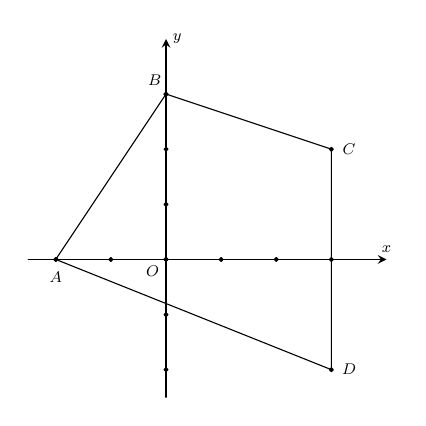
\begin{tikzpicture}[scale=.7,font=\footnotesize,line cap=round,line join=round,>=stealth]
		\path (-2,0)coordinate(A) (0,3)coordinate(B) (3,2)coordinate(C) (3,-2)coordinate(D);
		\foreach \i/\j in {A/-90,B/130,C/0,D/0}
		\draw[fill=black] (\i)node[shift=(\j:.32)]{$\i$}circle(1pt);
		\draw (A)--(B)--(C)--(D)--cycle;
		\draw[->] (-2.5,0)--(4,0)node[above]{$x$};
		\draw[->] (0,-2.5)--(0,4)node[right]{$y$};
		\foreach \i in {-2,-1,0,1,2,3}
		\draw[fill=black] (\i,0)node{}circle(1pt);
		\foreach \i in {-2,-1,0,1,2,3}
		\draw[fill=black] (0,\i)node{}circle(1pt);
		\draw (0,0)node[below left]{$O$};
	\end{tikzpicture}
}
\loigiai{
	Nhận thấy hình tứ giác $ABCD$ tính cả $4$ cạnh của nó là miền nghiệm của hệ bất phương trình gồm $4$ bất phương trình có miền nghiệm là nửa mặt phẳng chứa điểm $O(0;0)$ và lần lượt có các bờ là các đường $AB$, $BC$, $CD$ và $DA$.\\
	Phương trình đường thẳng $AB\colon -3x+2y=6$. Bất phương trình có miền nghiệm là nửa mặt phẳng bờ $AB$ (tính cả bờ $AB$) và chứa điểm $O$ là $-3x+2y\leq 6$.\\
	Phương trình đường thẳng $BC\colon x+3y=9$. Bất phương trình có miền nghiệm là nửa mặt phẳng bờ $BC$ (tính cả bờ $BC$) và chứa điểm $O$ là $x+3y\leq 9$.\\
	Phương trình đường thẳng $CD\colon x=3$. Bất phương trình có miền nghiệm là nửa mặt phẳng bờ $CD$ (tính cả bờ $CD$) và chứa điểm $O$ là $x\leq 3$.\\
	Phương trình đường thẳng $DA\colon 2x+5y=-4$. Bất phương trình có miền nghiệm là nửa mặt phẳng bờ $DA$ (tính cả bờ $DA$) và chứa điểm $O$ là $2x+5y\geq -4$.\\
	Như vậy hình tứ giác $ABCD$ tính cả $4$ cạnh của nó là miền nghiệm của hệ bất phương trình 
	$\heva{& -3x+2y\leq 6 \\ & x+3y\leq 9 \\& x\leq 3 \\ & 2x+5y\geq -4 }$ (*).\\
	Điểm $M( m;m+1 )$ nằm trên hình tứ giác $ABCD$ tính cả bốn cạnh của nó khi và chỉ khi $(m;m+1)$ là một nghiệm của hệ (*), tức là 
	\[\heva{& -3m+2(m+1)\leq 6 \\& m+3(m+1)\leq 9 \\ & m\leq 3 \\ & 2m+5( m+1 )\geq -4}\Leftrightarrow \heva{& m\geq -4 \\ & m\leq \dfrac{3}{2} \\ & m\leq 3 \\ & m\geq -\dfrac{9}{7}}\Leftrightarrow -\dfrac{9}{7}\leq m\leq \dfrac{3}{2}.\]
	Vậy các giá trị $m$ cần tìm là $-\dfrac{9}{7}\leq m\leq \dfrac{3}{2}$.
}
\end{bt}

% từ: cau-hoi/lop10/0H9_Phuong_phap_toa_do_trong_mat_phang/0H9-3-8_Bai_toan_thuc_te_PP_toa_do_hoa.tex
\begin{bt}%[0H9H3-8]%[ma:78b0318d]
Đường thẳng $\Delta$ ở hình bên dưới biểu thị tổng chi phí lắp đặt và tiền cước sử dụng dịch vụ Internet (đơn vị: trăm nghìn đồng) theo thời gian của một gia đình (đơn vị: tháng). Tính tổng chi phí (nghìn đồng) để lắp đặt và sử dụng Internet trong $12$ tháng đầu tiên.
\begin{center}
		\begin{tikzpicture}[scale=0.8, font=\footnotesize, line join=round, line cap=round, >=stealth]
			\draw[->,line width = 1pt] (-1,0)--(0,0) node[below left]{$O$}--(6.5,0) node[below]{$x$};
			\draw[->,line width =1 pt] (0,-1)--(0,5) node[right]{$y$};
			\draw [thick,domain=0:6,samples=100] 
			plot (\x,{(3/5)*(\x)+1/2}) node [above left] {$\Delta$};
			\draw (0,0.5) node [left] {$5$} circle (1pt);
			\draw (0,1) node [left] {$10$} circle (1pt);		
			\draw (0,2) node [left] {$20$} circle (1pt);
			\draw (0.5,0) node [below] {$1$} circle (1pt);
			\draw (2.5,0) node [below] {$5$} circle (1pt);
			\draw (6,0) node [below] {$12$} circle (1pt);
			\draw [dashed] (2.5,0)--(2.5,2)--(0,2);
		\end{tikzpicture}	
\end{center}
\shortans[]{$41$}
	\loigiai{
		\begin{itemize}
			\item Đường thẳng $\Delta$ đi qua hai điểm lần lượt có tọa độ $(0;\,5)$ và $(5;\,20)$ nên $\Delta$ có phương trình là
			$$\dfrac{x-0}{5-0}=\dfrac{y-5}{20-5}\Leftrightarrow\dfrac{x}{5}=\dfrac{y-5}{15}\Leftrightarrow\dfrac{x}{1}=\dfrac{y-5}{3}\Leftrightarrow3x-y+5=0\Leftrightarrow y=3x+5.$$
			\item $12$ tháng đầu tiên ứng với $x=12$. Do đó $y=3\cdot12+5=41$.\\
			Vậy tổng chi phí lắp đặt và sử dụng Internet trong $12$ tháng đầu tiên là $4100000$ đồng.
		\end{itemize}
		
	}
\end{bt}

% từ: cau-hoi/lop11/1C2_Ly_thuyet_do_thi/1C2-1-3_Cau_hoi_tong_hop.tex
\begin{ex}%[1C2B1-3]%[ma:a6658abb]
	Trong các dãy số $\left(u_n\right)$ sau đây, dãy số  nào là dãy số tăng?
	 \choice
		{$u_n=\sin  n$}
		{$u_n=n(-1)^n$} 
		 {$u_n=\dfrac{1}{n}$}
		{\True $u_n=2^{n+1}$} 
	 \loigiai{
		Xét dãy số $\left(u_n\right)$ cho bởi $u_n=2^{n+1}$.\\ 
		Ta có $u_n>0$ và $\dfrac{u_{n+1}}{u_n}=2>1$ nên $\left(u_n\right)$ là dãy  số tăng.
	} 
\end{ex}

% từ: cau-hoi/lop11/1D1_Ham_so_luong_giac_va_phuong_trinh_luong/1D1-1-2_Chuyen_doi_don_vi_do_va_radian.tex
\begin{ex}%[1D1B1-2]%[ma:bc4cd830]
	Hàm số $y=\sin x$ đồng biến trong  khoảng nào sau đây?
	 \choice
		 {$\left(7\pi; \dfrac{15\pi}{2}\right)$}
		{$\left(-\dfrac{7\pi}{2}; -3\pi\right)$} 
		{\True  $\left(\dfrac{19\pi}{2}; 10\pi\right)$}
		{$\left(-6\pi; -5\pi \right)$} 
	\loigiai{ Hàm số $y=\sin x$ đồng biến trên từng khoảng $\left(-\dfrac{\pi}{2}+k2\pi; \dfrac{\pi}{2}+k2\pi \right), k\in \mathbb{Z}$.\\ Dễ thấy với $k=5$ thì $\left(\dfrac{19\pi}{2};  10\pi\right)\subset \left(-\dfrac{\pi}{2}+5\cdot 2\pi; \dfrac{\pi}{2}+5\cdot 2\pi \right)$. Vậy $y=\sin x$ đồng biến trong khoảng $\left(\dfrac{19\pi}{2}; 10\pi\right)$. }
\end{ex}

% từ: cau-hoi/lop11/1D1_Ham_so_luong_giac_va_phuong_trinh_luong/1D1-1-3_So_do_cua_mot_goc_luong_giac.tex
\begin{ex}%[1D1N1-3]%[ma:74ddc1e8]
	Trong  các đẳng thức sau, đẳng thức nào đúng?
	 \choice
		 {$\cos 150^\circ =\dfrac{\sqrt{3}}{2} $}
		{$\cot 150^\circ =\sqrt{3} $} 
		{\True $\tan 150^\circ  =-\dfrac{1}{\sqrt{3}} $}
		 {$\sin 150{^\circ}=-\dfrac{\sqrt{3}}{2} $}
	 \loigiai{
		Khẳng định đúng là $\tan 150^\circ =-\dfrac{1}{\sqrt{3}} $. 
	} 
\end{ex}

% từ: cau-hoi/lop11/1D1_Ham_so_luong_giac_va_phuong_trinh_luong/1D1-1-3_So_do_cua_mot_goc_luong_giac.tex
\begin{ex}%[1D1H1-3]%[ma:7294a26c]
	 Hàm số nào sau đây là hàm số chẵn?
	 \choice
		{$y=\sin  x$}
		{$y=\tan x$} 
		{\True $y=\cos  x$}
		 {$y=\cot x$}
	 \loigiai{
		Theo tính chất ta có hàm số $y=\sin x$, $y=\tan x$, $y=\cot x$ là hàm số lẻ;  hàm số $ y=\cos x$ là hàm số chẵn.
	} 
\end{ex}

% từ: cau-hoi/lop11/1D1_Ham_so_luong_giac_va_phuong_trinh_luong/1D1-2-1_Cau_hoi_ly_thuyet.tex
\begin{ex}%[1D1B2-1]%[ma:892faf0e]
	Phương trình  lượng giác: $2\cos x+\sqrt{2}=0$ có nghiệm là
	\choice 
		 {$\hoac{&x=\dfrac{\pi}{4}+k2\pi\\&x=-\dfrac{\pi}{4}+k2\pi}$}
		{\True  $\hoac{&x=\dfrac{3\pi}{4}+k2\pi\\&x=-\dfrac{3\pi}{4}+k2\pi}$}
		{$\hoac{&x=\dfrac{\pi}{4}+k2\pi\\&x=\dfrac{3\pi}{4}+k2\pi}$} 
		{$\hoac{&x=\dfrac{7\pi}{4}+k2\pi\\&x=-\dfrac{7\pi}{4}+k2\pi}$} 
	\loigiai{ 
		$2\cos  x+\sqrt{2}=0\Leftrightarrow \cos x =-\dfrac{\sqrt{2}}{2}\Leftrightarrow \hoac{&x=\dfrac{3\pi}{4}+k2\pi\\&x=-\dfrac{3\pi}{4}+k2\pi.}$
	 }
\end{ex}

% từ: cau-hoi/lop11/1D1_Ham_so_luong_giac_va_phuong_trinh_luong/1D1-2-1_Cau_hoi_ly_thuyet.tex
\begin{ex}%[1D1Y2-1]%[ma:f4368a76]
	Nghiệm âm lớn nhất của phương  trình $\sin 2x=\dfrac{\sqrt{3}}{2}$ là
	\choice 
		 {$-\dfrac{\pi}{6}$}
		{ $-\dfrac{5\pi}{6}$} 
		 {\True$-\dfrac{2\pi}{3}$}
		 {$-\dfrac{\pi}{3}$}
	\loigiai{$\sin 2x=\dfrac{\sqrt{3}}{2}\Leftrightarrow \hoac{&2x=\dfrac{\pi}{3}+k2\pi\\&2x=\dfrac{2\pi}{3}+k2\pi}\Leftrightarrow \hoac{&x=\dfrac{\pi}{6}+k\pi\\&x=\dfrac{\pi}{3}+k\pi  } ,\, k\in \mathbb{Z}$.\\
	Vậy nghiệm âm lớn nhất  của phương trình là $x=-\dfrac{2\pi}{3}$.}
\end{ex}

% từ: cau-hoi/lop11/1D1_Ham_so_luong_giac_va_phuong_trinh_luong/1D1-2-1_Cau_hoi_ly_thuyet.tex
\begin{ex}%[1D1B2-1]%[ma:07120fff]
	Phương trình $\left( \sqrt{3}\tan x +1\right)\left(\sin^2x+1\right) =0$ có  nghiệm là
	\choice 
		{$x= -\dfrac{\pi}{6} +k2\pi$} 
		{$x= \dfrac{\pi}{6}  +k\pi$}
		{$x=  \dfrac{\pi}{3} +k2\pi$}
		{\True $x= -\dfrac{\pi}{6} +k\pi$} 
	\loigiai{  Ta có
		$\left( \sqrt{3}\tan x +1\right)\left(\sin^2x+1\right) =0 \Leftrightarrow \tan x = -\dfrac{1}{\sqrt{3}} \Leftrightarrow x= -\dfrac{\pi}{6}  +k\pi.$
	 }
\end{ex}

% từ: cau-hoi/lop11/1D1_Ham_so_luong_giac_va_phuong_trinh_luong/1D1-2-1_Cau_hoi_ly_thuyet.tex
\begin{ex}%[1D1B2-1]%[ma:f2e52dbc]
	Tổng  các nghiệm của phương trình $\sin x=\dfrac{-1}{2\sqrt{2}\cos x}$ trên đoạn $\left[0;2\pi\right]$ có dạng $a \pi$. Khi đó $a$ bằng
	 \shortans{5}
	\loigiai{ 
		Điều kiện $\cos  x\neq 0\Leftrightarrow x\neq\dfrac{\pi}{2}+k\pi, k\in\mathbb{Z}$.\\
		 Ta có
		\begin{eqnarray*}
			\sin x=\dfrac{-1}{2\sqrt{2}\cos x} 
			 &\Leftrightarrow &2\sin x\cos x =-\dfrac{1}{\sqrt{2}}\\
			&\Leftrightarrow  &\sin2x =\sin\left(-\dfrac{\pi}{4}\right)\\
			&\Leftrightarrow &\hoac{&x=-\dfrac{\pi}{8}+k\pi\\&x=\dfrac{5\pi}{8}+k\pi},  k \in \mathbb{Z}.
		\end{eqnarray*}
		Trên đoạn $[0;2\pi]$ phương trình có các nghiệm là $\dfrac{7\pi}{8}, \dfrac{15\pi}{8}, \dfrac{5\pi}{8}, \dfrac{13\pi}{8}$.\\ 
		Vậy tổng  các nghiệm trên đoạn $[0;2\pi]$ là $5\pi$.
	 }
\end{ex}

% từ: cau-hoi/lop11/1D1_Ham_so_luong_giac_va_phuong_trinh_luong/1D1-2-2_Xet_dau_gia_tri_luong_giac_Tinh_gia_tri_luong.tex
\begin{ex}%[1D1H2-2]%[ma:0fa3624c]
	Giá trị của biểu thức $ S=3-\sin^290^\circ+2\cos^260^\circ-3\tan^245^\circ $ bằng 
	 \choice
		{$\dfrac{1}{2}$} 
		{\True  $-\dfrac{1}{2}$}
		{$  1$}
		{$  3$}
	\loigiai{Ta có $  S=3-\sin^290^\circ+2\cos^260^\circ-3\tan^245^\circ =3-1^2+2\cdot \left(\dfrac{1}{2}\right)^2-3\cdot 1^2=-\dfrac{1}{2}$.}
\end{ex}

% từ: cau-hoi/lop11/1D1_Ham_so_luong_giac_va_phuong_trinh_luong/1D1-2-3_Bien_doi_rut_gon_bieu_thuc_luong_giac_chung_m.tex
\begin{ex}%[1D1V2-3]%[ma:76286a91]
	\immini[thm]{Cho hai điểm $A$, $B$ thuộc đồ  thị hàm số $y=\sin x$ trên đoạn $[0;\pi]$, các điểm $C$, $D$ thuộc trục $Ox$ thỏa mãn $ABCD$ là hình chữ nhật và $CD=\dfrac{2\pi}{3}$. Tính độ dài đoạn $BC$.
	\shortans{18,8} 
	}{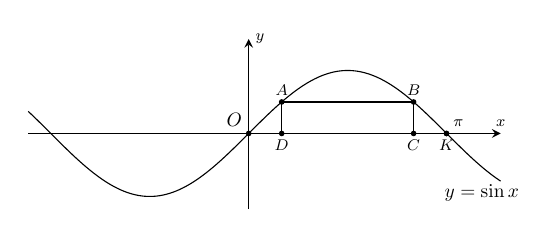
\begin{tikzpicture}[>=stealth,x=1.0cm,y=1.0cm,scale=0.8]
		\draw[->](-3.5,0) --  (4,0) node[above]{\footnotesize $x$};
		\draw[->](0,-1.2) -- (0,1.5)  node[right]{\footnotesize $y$};
		\draw[fill=black] (0,0) node [above left]{$O$} circle (1pt); 
		 \draw[fill=black] (3.14,0) node [above right]{\footnotesize $\pi$} circle (1pt);
		\draw[fill=black] (3.14,0) node [below]{\footnotesize $K$}  circle (1pt);
		\draw[smooth,samples=100,domain=-3.5:4]plot (\x,{sin  ((\x)*180/pi)});
		\draw (pi/6,0)--(pi/6,0.5)--(5*pi/6,0.5)--(5*pi/6,0); 
		\draw[fill=black] (pi/6,0) node [below]{\footnotesize $D$} circle  (1pt);
		\draw[fill=black](pi/6,0.5) node [above]{\footnotesize $A$}  circle (1pt);
		\draw[fill=black] (5*pi/6,0.5) node [above]{\footnotesize  $B$} circle (1pt);
		\draw[fill=black] (5*pi/6,0)  node [below]{\footnotesize $C$} circle (1pt);
		\node at  (3.7,-0.7) [below]{$y=\sin x$};
	\end{tikzpicture}
	} 
	 \loigiai{
		Theo hình vẽ thì $OD=CK \Rightarrow 2OD=\pi-CD=\dfrac{\pi}{3}\Rightarrow OD=\dfrac{\pi}{6}\Rightarrow x_D=\dfrac{\pi}{6}$.\\ 
		Tung độ điểm $D$ là $y_D=\sin\left(\dfrac{\pi}{6} \right)=\dfrac{1}{2}=AD=BC$. 
	} 
\end{ex}

% từ: cau-hoi/lop11/1D1_Ham_so_luong_giac_va_phuong_trinh_luong/1D1-2-4_Cac_goc_luong_giac_co_lien_quan_dac_biet_bu_n.tex
\begin{ex}%[1D1N2-4]%[ma:21426de1]
	 Giá trị của biểu thức $S=3-\sin ^290^{\circ}+2\cos ^260^{\circ}-3\tan ^245^{\circ}$ bằng
	 \choice
		{$\dfrac{1}{2}$} 
		{\True  $-\dfrac{1}{2}$}
		{$1$} 
		{$3$} 
	\loigiai{ 
		Ta có $S=3-\sin ^290^{\circ}+2\cos ^260^{\circ}-3\tan ^245^{\circ}$  $=3-1^2+2\cdot \left(\dfrac{1}{2} \right)^2-3\cdot 1^2$ $=-\dfrac{1}{2}$.
	} 
\end{ex}

% từ: cau-hoi/lop11/1D1_Ham_so_luong_giac_va_phuong_trinh_luong/1D1-3-2_Ap_dung_cong_thuc_cong.tex
\begin{bt}%[1D1V3-2]%[ma:cfa9cf60]
% nguon: Archive/SP_KhoLatex/ID6_old/1K1-2.tex #3579
%[Dự án 1 - TLDH - TeamTeXHoa - DiaMond]
Rút gọn biểu thức $A=\sin(x+14^\circ)\sin(x+74^\circ)+\sin(x-76^\circ)\sin(x-16^\circ)$. 
\loigiai{
Ta có
\begin{eqnarray*}
A&=&\sin(14^\circ+x)\cos(16^\circ-x)+\sin(76^\circ-x)\sin(16^\circ-x)\\
&=&\sin(14^\circ+x)\cos(16^\circ-x)+\cos(14^\circ+x)\sin(16^\circ-x)\\
&=&\sin(14^\circ+16^\circ+x-x)\\
&=&\sin30^\circ=\dfrac{1}{2}.
\end{eqnarray*}
}
\end{bt}

% từ: cau-hoi/lop11/1D1_Ham_so_luong_giac_va_phuong_trinh_luong/1D1-3-4_Ap_dung_cong_thuc_bien_doi_tich_tong.tex
\begin{ex}%[1D1H3-4]%[ma:c9677f10]
	 Biểu thức $A=\dfrac {1}{2\sin 10^\circ}-2\sin 70^\circ$ có giá trị đúng bằng
	\choice 
		{\True  $1$}
		{$1$} 
		{$2$} 
		 {$3$}
	 \loigiai{
		\allowdisplaybreaks 
		\begin{align*}
			A&=\dfrac {1}{2\sin  10^\circ}-2\sin 70^\circ\\
			&=\dfrac {1-4\sin 10^\circ \cdot \sin 70^\circ}{2\sin  10^\circ}\\
			 &=\dfrac {2\sin 80^\circ}{2\sin 10^\circ}\\
			&=\dfrac  {2\sin 10^\circ}{2\sin 10^\circ}\\
			&=1. 
		\end{align*}
	} 
\end{ex}

% từ: cau-hoi/lop11/1D1_Ham_so_luong_giac_va_phuong_trinh_luong/1D1-3-4_Ap_dung_cong_thuc_bien_doi_tich_tong.tex
\begin{bt}%[1D1H3-4]%[ma:a46617e0]
% nguon: Archive/2024/SP-K10-K11-LyVanHoang_TVN-023/11. C1-LuongGiac-lvhoang_TVN-023/dataC1K11/Bai2-Dang3-Congthucbiendoitichthanhtong.tex #1786
%[Huỳnh Đức Vũ, dự án bài giảng K10-11]
	Cho $\cos 2 x=\dfrac{1}{4}$. Tính 
	\begin{listEX}[2]
		\item $A=\cos \left(x+\dfrac{\pi}{6}\right) \cos \left(x-\dfrac{\pi}{6}\right)$.
		\item $B=\sin \left(x+\dfrac{\pi}{3}\right) \sin \left(x-\dfrac{\pi}{3}\right)$.  	
	\end{listEX}   
	\loigiai{
		\begin{listEX}
			\item $A=\dfrac{1}{2}\left(\cos 2 x+\cos \dfrac{\pi}{3}\right)=\dfrac{1}{2}\left(\dfrac{1}{4}+\dfrac{1}{2}\right)=\dfrac{3}{8}$.
			\item $B=-\dfrac{1}{2}\left(\cos 2 x-\cos \dfrac{2\pi}{3}\right)=-\dfrac{1}{2}\left(\dfrac{1}{4}+\dfrac{1}{2}\right)=-\dfrac{3}{8}$.			
		\end{listEX}
	}
\end{bt}

% từ: cau-hoi/lop11/1D1_Ham_so_luong_giac_va_phuong_trinh_luong/1D1-3-5_Ket_hop_nhieu_cong_thuc_luong_giac.tex
\begin{ex}%[1D1V3-5]%[ma:0e8bb76b]
	Cho biết $\cos\alpha=-\dfrac{2}{3}$. Giá trị của  biểu thức $P=\dfrac{\cot\alpha+3\tan\alpha}{2\cot\alpha+\tan\alpha}$ bằng bao nhiêu?
	 \choice
		 {\True $P=\dfrac{19}{13}$}
		 {$P=\dfrac{25}{13}$}
		{$P=-\dfrac{25}{13}$} 
		{$P=-\dfrac{19}{13}$} 
	\loigiai{ 
		Ta có  $\cos\alpha=-\dfrac{2}{3}\Rightarrow{\tan ^2}\alpha=\dfrac{1}{\cos^2\alpha}-1=\dfrac{1}{\left(\dfrac{-2}{3}\right)^2}-1=\dfrac{5}{4}$.\\
		$P=\dfrac{\cot\alpha+3\tan\alpha}{2\cot\alpha+\tan\alpha}=\dfrac{\dfrac{1}{\tan\alpha}+3\tan\alpha}{\dfrac{2}{\tan\alpha}+\tan\alpha}=\dfrac{\dfrac{1+3\tan^2\alpha}{\tan\alpha}}{\dfrac{2+\tan^2\alpha}{\tan\alpha}}=\dfrac{1+3\tan^2\alpha}{2+\tan^2\alpha}=\dfrac{1+3\cdot\dfrac{5}{4}}{2+\dfrac{5}{4}}=\dfrac{19}{13}$. 
	 }
\end{ex}

% từ: cau-hoi/lop11/1D1_Ham_so_luong_giac_va_phuong_trinh_luong/1D1-3-5_Ket_hop_nhieu_cong_thuc_luong_giac.tex
\begin{ex}%[1D1V3-5]%[ma:b5902086]
	Tính giá trị của biểu thức $M=\cos^4{15^\circ}-\sin ^4{15^\circ}+\cos^2{15^\circ}-\sin^2{15^\circ}$ (làm trong  đến hàng phần trăm).
	 \shortans{1,73}
	 \loigiai{
	Áp dụng công thức nhân đôi  $\cos ^2a-\sin ^2a=\cos 2a$ .\\
	Ta  có
	\begin{align*}
		M&\,=\left(\cos^415^{\circ}-\sin^415^{\circ}\right)+\left(\cos^215^{\circ}-\sin^215^{\circ}\right)\\ 
		 &\,=\left(\cos^215^{\circ}-\sin^215^{\circ}\right)\left(\cos^215^{\circ}+\sin^215^{\circ}\right)+\left(\cos^215^{\circ}-\sin^215^{\circ}\right)\\
		&\,=\left(\cos^215^{\circ}-\sin^215^{\circ}\right)+\left(\cos^215^{\circ}-\sin^215^{\circ}\right)\\ 
		 &\,=\cos{30^{\circ}}+\cos{30^{\circ}}=\sqrt 3.
	\end{align*}
	} 
\end{ex}

% từ: cau-hoi/lop11/1D1_Ham_so_luong_giac_va_phuong_trinh_luong/1D1-3-6_Nhan_dang_tam_giac.tex
\begin{bt}%[1D1V3-6]%[ma:22f3ed2c]
% nguon: Archive/SP_KhoLatex/ID6_old/1K1-2-3.tex #3316
%%[DCHT Toán 11 - KNTT -Nguyễn Thành Nhân] 
	Cho tam giác $ABC$ có ba góc $A$, $B$, $C$ thỏa mãn hệ thức $\sin A=\cos B+\cos C$. Chứng minh rằng tam giác $ABC$ là tam giác vuông.
	\loigiai{
		Ta có
		\allowdisplaybreaks
		\begin{eqnarray*}
			& &\sin A=\cos B+\cos C\\
			&\Leftrightarrow & 2\sin \dfrac{A}{2}\cos \dfrac{A}{2}=2\cos \dfrac{B+C}{2}\cos \dfrac{B-C}{2}\\
			&\Leftrightarrow & 2\sin \dfrac{A}{2}\cos \dfrac{A}{2}=2\cos \left(\dfrac{\pi}{2}-\dfrac{A}{2}\right)\cos \dfrac{B-C}{2} \\
			&\Leftrightarrow & \cos \dfrac{A}{2}=\cos \dfrac{B-C}{2}.
		\end{eqnarray*}
		Suy ra $\hoac{&\dfrac{A}{2}=\dfrac{B-C}{2} \\& \dfrac{A}{2}=-\dfrac{B-C}{2}}\Rightarrow \hoac{&B=A+C \\& C=A+B.}$\\
		Vậy tam  giác $ABC$ vuông tại $B$ hoặc tại $C$.}
\end{bt}

% từ: cau-hoi/lop11/1D1_Ham_so_luong_giac_va_phuong_trinh_luong/1D1-3-7_Toan_thuc_te_ap_dung_cong_thuc_luong_giac.tex
\begin{ex}%[1D1V3-7]%[ma:65017bb2]
	Một sợi cáp $ R$ được gắn vào một cột thẳng đứng ở vị trí cách mặt đất $ 14\;$m. Một sợi cáp $ S$ khác cũng được gắn vào cột đó ở vị trí cách mặt đất $ 12\;$m. Biết rằng hai sợi cáp  trên cùng được gắn với mặt đất tại một vị trí cách chân cột $15$ m.
	\begin{center}
		\begin{tikzpicture}[scale=0.8,line join=round,line cap=round,>=stealth]
				\coordinate (A)  at (0,0);
				\coordinate  (B) at (0,6);
				 \coordinate (C) at (3,6);
				\coordinate (D) at  (3,0);
				\coordinate (E) at (2,0); 
				 \coordinate (F) at (2,4);
				\coordinate (G)  at (6,7);
				\coordinate (H) at  (6,1);
				\coordinate (I)  at (3,4);
				\coordinate (J) at (6,5); 
				\coordinate (K) at (11,0); 
				\draw [<->,dashed] (A)--(B) node[midway,left] {14m} 
					(E)--(F)  node[midway,left] {12m};
				\draw [dashed] (A)--(D) 
					(F)--(I) 
					(B)--(C); 
				\draw (D) --  (K) node[midway,below,sloped] {15m};
				\draw[line  width=1.8pt] (D) -- (C)
					(H)--(G); 
				\draw (C)--(G) 
					 (I)--(J)
					 (D)--(H)
					(I)--(K)  node[midway,below,sloped] {S}
					(K)--(C) node[midway,above,sloped]  {R};
				\pic [draw,angle radius=1cm,"$\alpha$",angle eccentricity=1.3]  {angle = C--K--I};
				\draw (D) node[below]{H} 
					(I) node[above  left]{B}
					(C)  node[above]{A}
					(K)  node[below]{O};
			\end{tikzpicture}
	\end{center}
	\begin{enumerate}
		\item Tính $\tan{\alpha}$ với $\alpha$ là góc  giữa hai sợi cáp trên.
		\item Tính số đo  góc $\alpha$ (làm tròn kết quả đến hàng đơn vị theo độ).
	\end{enumerate}
	 \loigiai{
	\begin{enumerate}
		\item Ta  có $\alpha=\widehat{AOH}-\widehat{BOH}$.\\
		Trong tam giác vuông $ AOH$  ta có $\tan\widehat{AOH}=\dfrac{AH}{OH}=\dfrac{14}{15}$.\\
		Trong tam  giác vuông $ BOH$ ta có $\tan\widehat{BOH}=\dfrac{BH}{OH}=\dfrac{12}{15}=\dfrac{4}{5}$.\\
		 Vậy $\tan\alpha=\tan\left(\widehat{AOH}-\widehat{BOH}\right)=\dfrac{\tan\widehat{AOH}-\tan\widehat{BOH}}{1+\tan\widehat{AOH}\cdot\tan\widehat{BOH}}=\dfrac{\dfrac{14}{15}-\dfrac{4}{5}}{1+\dfrac{14}{15}\cdot\dfrac{4}{5}}=\dfrac{10}{131}$.
		\item Từ kết  quả câu a ta có $\alpha\approx 4^{\circ} $.
	\end{enumerate}
	 }
\end{ex}

% từ: cau-hoi/lop11/1D1_Ham_so_luong_giac_va_phuong_trinh_luong/1D1-4-7_Bang_bien_thien_va_do_thi.tex
\begin{bt}%[1D1H4-7]%[ma:84168d87]
% nguon: Archive/SP_KhoLatex/ID6_old/1K1-3.tex #3550
%[Dự án 1 - TLDH - TeamTeXHoa - Trần Trọng Tiên]
	Vẽ đồ thị hàm số $y=\cos\dfrac{x}{3}$.
	\loigiai{
		Miền xác định: $\mathscr{D}=\mathbb{R}$.\\
		Ta chỉ cần vẽ đồ thị hàm số trên miền $\left[0 ; 6\pi\right]$ (do chu kì tuần hoàn $T=2\pi:\dfrac{1}{3}=6\pi$).\\
		Bảng giá trị của hàm số $y=\cos\dfrac{x}{3}$ trên đoạn $\left[0 ; 6\pi\right]$ là
		\begin{center}
			\setlength\extrarowheight{10pt}
			\begin{tabular}{|c|c|c|c|c|c|c|c|c|c|}
				\hline
				$x$	& $0$ &$\dfrac{3\pi}{4}$  & $\dfrac{3\pi}{2}$ & $\dfrac{21\pi}{6}$ & $3\pi$  & $\dfrac{15\pi}{4}$ & $\dfrac{9\pi}{2}$ &$\dfrac{33\pi}{6}$  & $6\pi$ \\
				\hline
				$y$	& $1$  & $\dfrac{\sqrt{2}}{2}$ & $0$ & $-\dfrac{\sqrt{3}}{2}$ & $-1$ & $-\dfrac{\sqrt{2}}{2}$  & $0$ & $\dfrac{\sqrt{3}}{2}$ & $1$ \\
				\hline
			\end{tabular}
		\end{center}
		Ta có đồ thị của hàm số $y=\cos\dfrac{x}{3}$ trên đoạn  $\left[0 ; 6\pi\right]$ và sau đó tịnh tiến cho các đoạn: $\ldots,\left[-6\pi ; 0\right],\left[6\pi; 12\pi\right],\ldots$
	}
	\begin{center}
		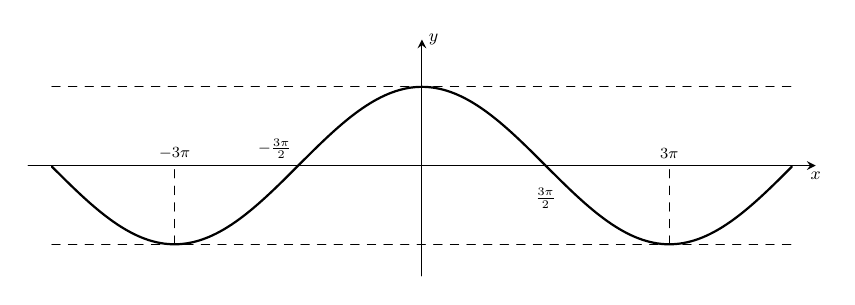
\begin{tikzpicture}[scale=1, font=\footnotesize, line join=round, line cap=round, >=stealth]
			\draw[->] (-5,0) -- (5,0) node[below] {\small $x$};
			\draw[->] (0,-1.4)-- (0,1.6) node[right] {\small $y$};
			\draw[thick,samples=100,domain=-4.7:4.7] plot(\x,{cos((\x)*180/pi)});
			\draw[dashed] (-3.14,-1)--(-3.14,0) node[above] {$-3\pi$};
			\draw[dashed] (3.14,-1)--(3.14,0) node[above] {$3\pi$};
			\draw (-1.57,0) node[above left] {$-\frac{3\pi}{2}$};
			\draw (1.57,-0.2) node[below] {$\frac{3\pi}{2}$};
			\draw[dashed] (-4.7,1)--(4.7,1);
			\draw[dashed] (-4.7,-1)--(4.7,-1);
			
		\end{tikzpicture}
	\end{center}
\end{bt}

% từ: cau-hoi/lop11/1D1_Ham_so_luong_giac_va_phuong_trinh_luong/1D1-4-8_Toan_thuc_te_ap_dung_ham_so_luong_giac.tex
\begin{ex}%[1D1V4-8]%[ma:67ed31ca]
	\immini[thm]{Người ta nghiên cứu sự sinh trưởng và phát triển của một loại sinh vật $A$ trên một hòn đảo thì thấy sinh vật $A$ phát triển theo quy luật $$s(t)=a+b\sin\dfrac{\pi t}{18},\  a,b\in\mathbb{R}$$ với $s(t)$ là số lượng sinh vật $A$ sau $t$ năm và có đồ thị như hình vẽ.}
	{ 
	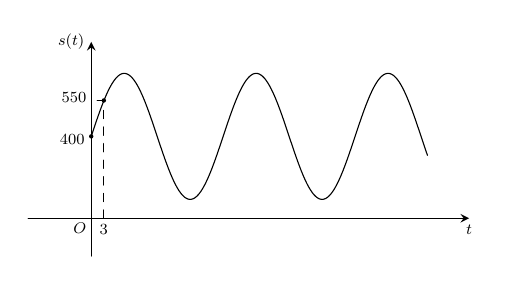
\begin{tikzpicture}[scale=0.8,font=\footnotesize,line join=round,line cap=round,>=stealth]
			\draw[->]  (-1,0)--(6,0) node [below]{$t$};
			\draw[->] (0,-0.6)--(0,2.8) node [left]{$s  (t)$};
			\node at (0,0) [below left=-1pt]{$O$}; 
			 \draw plot[samples=300,domain=0:1.7*pi](\x,{1.3+sin (3*\x r)});
			\fill (0,1.3) circle (1pt) node[shift={(-170:10pt)}]{$400$}; 
			\fill (0.2,1.27+sin 0.6r) circle  (1pt);
			\draw[dashed] (0.2,0)  node[shift={(-90:6pt)}]{$3$}|-(0,1.27+sin 0.6r) node[shift={(170:9pt)}]{$550$};
		\end{tikzpicture}
	 }
	Hỏi số lượng sinh vật  $A$ được nhiều nhất bao nhiêu con?
	 \shortans{700}
	 \loigiai{
		Dựa vào đồ thị ta  thấy $\heva{
		&s(0)=400\\ 
		&s(3)=550\\}\Rightarrow\heva{ 
		&a=400\\ 
		 &b=550.\\}$\\
		Suy ra  $s(t)=400+300\sin\dfrac{\pi}{18}t$.\\
		Ta có $$-1\leq \sin\dfrac{\pi}{18}t\leq 1\Leftrightarrow-300\leq 300\sin\dfrac{\pi}{18}t\leq 300\Leftrightarrow 100 \leq  400+ 300\sin\dfrac{\pi}{18}t\leq 700\ (\forall t\geq 0).$$
		Vậy số lượng sinh vật  nhiều nhất là $700$ con.
	 }
\end{ex}

% từ: cau-hoi/lop11/1D1_Ham_so_luong_giac_va_phuong_trinh_luong/1D1-5-3_Phuong_trinh_co_ban_dung_Radian.tex
\begin{bt}%[1D1H5-3]%[ma:e7086add]
% nguon: Archive/2024/SP-K10-K11-LyVanHoang_TVN-023/11. C1-LuongGiac-lvhoang_TVN-023/dataC1K11/Chuong1-Bai4-Dang3-PhuongTrinhCBDungRadian.tex #1629
[Mức H, CTST]%[BG Toán 11 CT2025, Quan Ón] 
	Giải các phương trình
	\begin{listEX}[3]
		\item $\sin x=-\dfrac{3}{2}$;
		\item $\sin x=\dfrac{\sqrt{3}}{2}$;
		\item $\cos x=-3$;
		\item $\cos\left(x+\dfrac{\pi}{12}\right)=\cos\dfrac{3\pi}{12}$;
		\item $\tan2x=\tan\dfrac{\pi}{11}$;
		\item $\tan x=0$;
		\item $\cot3x=\cot\dfrac{\pi}{7}$;
		\item $\cot x=1$;
		\item $\sin2x=\sin3x$;
		\item $\cos3x=\sin x$.
	\end{listEX}
	\loigiai{
		\begin{enumerate}
			\item $\sin x=-\dfrac{3}{2}$ vô nghiệm vì $\left|-\dfrac{3}{2} \right| = \dfrac{3}{2} > 1$.
			\item $\sin x=\dfrac{\sqrt{3}}{2}\Leftrightarrow\sin x=\sin\dfrac{\pi}{3}\Leftrightarrow\hoac{&x=\dfrac{\pi}{3}+k2\pi\\&x=\dfrac{2\pi}{3}+k2\pi}\,(k\in\mathbb{Z})$.
			\item $\cos x=-3$ vô nghiệm vì $|-3| = 3 > 1$.
			\item $\cos\left(x+\dfrac{\pi}{12}\right)=\cos\dfrac{3\pi}{12}\Leftrightarrow\hoac{&x+\dfrac{\pi}{12}=\dfrac{3\pi}{12}+k2\pi\\&x+\dfrac{\pi}{12}=-\dfrac{3\pi}{12}+k2\pi}\Leftrightarrow\hoac{&x=\dfrac{\pi}{6}+k2\pi\\&x=-\dfrac{\pi}{3}+k2\pi}\,(k\in\mathbb{Z})$.
			\item $\tan2x=\tan\dfrac{\pi}{11}\Leftrightarrow2x=\dfrac{\pi}{11}+k\pi\Leftrightarrow x=\dfrac{\pi}{22}+\dfrac{k\pi}{2},\,(k\in\mathbb{Z})$.
			\item $\tan x=0 \Leftrightarrow x=k\pi,\,(k\in\mathbb{Z})$.
			\item $\cot3x=\cot\dfrac{\pi}{7}\Leftrightarrow 3x=\dfrac{\pi}{7}+k\pi\Leftrightarrow x=\dfrac{\pi}{21}+\dfrac{k\pi}{3},\,(k\in\mathbb{Z})$.
			\item $\cot x=1\Leftrightarrow\cot x=\cot\dfrac{\pi}{4}\Leftrightarrow x=\dfrac{\pi}{4}+k\pi,\,(k\in\mathbb{Z})$.
			\item $\sin2x=\sin3x\Leftrightarrow\hoac{&2x=3x+k2\pi\\&2x=\pi-3x+k2\pi}\Leftrightarrow\hoac{&x=-k2\pi\\&x=\dfrac{\pi}{5}+\dfrac{k2\pi}{5}}\,(k\in\mathbb{Z})$.
			\item $\cos3x=\sin x\Leftrightarrow \cos3x=\cos\left(\dfrac{\pi}{2}-x\right)\Leftrightarrow\hoac{&3x=\dfrac{\pi}{2}-x+k2\pi\\&3x=-\dfrac{\pi}{2}+x+k2\pi}\Leftrightarrow\hoac{&x=\dfrac{\pi}{8}+\dfrac{k\pi}{2}\\&x=-\dfrac{\pi}{4}+k\pi}\,(k\in\mathbb{Z})$.
	\end{enumerate}}
\end{bt}

% từ: cau-hoi/lop11/1D1_Ham_so_luong_giac_va_phuong_trinh_luong/1D1-5-3_Phuong_trinh_co_ban_dung_Radian.tex
\begin{bt}%[1D1H5-3]%[ma:7e759c1b]
% nguon: Archive/2024/SP-K10-K11-LyVanHoang_TVN-023/11. C1-LuongGiac-lvhoang_TVN-023/dataC1K11/Chuong1-Bai4-Dang3-PhuongTrinhCBDungRadian.tex #1634
[Mức H, KNTT]%[BG Toán 11 CT2025, Quan Ón]
	Giải các phương trình sau
	\begin{listEX}[3]
		\item $\sin x=\dfrac{\sqrt{3}}{2}$;
		\item $2\cos x=-\sqrt{2}$;
		\item $\cot(2x-1)=\cot\dfrac{\pi}{5}$.
	\end{listEX}
	\loigiai{
		\begin{enumerate}
			\item $\sin x=\dfrac{\sqrt{3}}{2}\Leftrightarrow\sin x=\sin\dfrac{\pi}{3}\Leftrightarrow \hoac{&x=\dfrac{\pi}{3}+k2\pi\\&x=\pi-\dfrac{\pi}{3}+k2\pi}\Leftrightarrow\hoac{&x=\dfrac{\pi}{3}+k2\pi\\&x=\dfrac{2\pi}{3}+k2\pi}\,(k\in\mathbb{Z})$.
			\item $2\cos x=-\sqrt{2}\Leftrightarrow\cos x=-\dfrac{\sqrt{2}}{2}\Leftrightarrow\cos x=\cos\dfrac{3\pi}{4}\Leftrightarrow x=\pm\dfrac{3\pi}{4}+k2\pi,\,(k\in\mathbb{Z})$.
			\item $\cot(2x-1)=\cot\dfrac{\pi}{5}\Leftrightarrow2x-1=\dfrac{\pi}{5}+k\pi\Leftrightarrow x=\dfrac{\pi}{10}+\dfrac{1}{2}+\dfrac{k\pi}{2},\,(k\in\mathbb{Z})$.
		\end{enumerate}
	}
\end{bt}

% từ: cau-hoi/lop11/1D1_Ham_so_luong_giac_va_phuong_trinh_luong/1D1-5-3_Phuong_trinh_co_ban_dung_Radian.tex
\begin{bt}%[1D1H5-3]%[ma:2ddf51e3]
% nguon: Archive/2024/SP-K10-K11-LyVanHoang_TVN-023/11. C1-LuongGiac-lvhoang_TVN-023/dataC1K11/Chuong1-Bai4-Dang4-PhuongTrinhCBDungDo.tex #1666
[Mức H, KNTT]%[BG Toán 11 CT2025, Quan Ón]
	Giải các phương trình sau
	\begin{listEX}[2]
		\item $\sin 2x  = \sin (60^{\circ} - 3x)$;
		\item $\cos 2 x=\cos \left(45^{\circ}-x\right)$.
	\end{listEX}
	\loigiai{
		\begin{enumerate}
			\item $\sin2x=\sin(60^{\circ}-3x)\Leftrightarrow\hoac{&2x=60^\circ-3x+k360^\circ\\&2x=3x+120^\circ+k360^\circ}\Leftrightarrow\hoac{&x=12^\circ+k72^\circ\\&x=-120^\circ-k360^\circ},\,(k \in \mathbb{Z})$.
			\item $\cos2x=\cos\left(45^{\circ}-x\right)  \Leftrightarrow\hoac{&2 x=45^{\circ}-x+k 360^{\circ}\\&2x=-\left(45^{\circ}-x\right)+k 360^{\circ}} \Leftrightarrow\hoac{&3x=45^{\circ}+k360^{\circ}\\&x=-45^{\circ}+k360^{\circ}}\\\Leftrightarrow \hoac{&x=15^{\circ}+k 120^{\circ} \\&x=-45^{\circ}+k 360^{\circ}},\,(k \in \mathbb{Z})$.
		\end{enumerate}
	}
	
\end{bt}

% từ: cau-hoi/lop11/1D1_Ham_so_luong_giac_va_phuong_trinh_luong/1D1-5-3_Phuong_trinh_co_ban_dung_Radian.tex
\begin{bt}%[1D1H5-3]%[ma:d5f14b40]
% nguon: Archive/SP_KhoLatex/ID6_old/11-OT-PTLuongGiacCoBan.tex #3092
%[ĐGNL-ĐGTD-2022, Tran Tony]
	Giải phương trình $\tan 2x=1$.
	\loigiai{
		Ta có
		$$\tan 2x=1 \Leftrightarrow  x=\dfrac{\pi}{8}+\dfrac{k\pi}{2}, k\in \mathbb{Z}.$$
	}
\end{bt}

% từ: cau-hoi/lop11/1D1_Ham_so_luong_giac_va_phuong_trinh_luong/1D1-5-3_Phuong_trinh_co_ban_dung_Radian.tex
\begin{bt}%[1D1H5-3]%[ma:13c72c3a]
% nguon: Archive/SP_KhoLatex/ID6_old/GK1.6.tex #3330

	Giải phương trình $2\sin x-1=0$.
	\loigiai{
	Ta có:
	\begin{eqnarray*}
		&& 2\sin x-1=0\Leftrightarrow 2\sin x=1 \\
		& \Leftrightarrow& \sin x=\dfrac{1}{2}=\sin \dfrac{\pi}{6}\\
		&\Leftrightarrow& \hoac{& x=\dfrac{\pi}{6}+k2\pi \\
		& x=\pi-\dfrac{\pi}{6}+k2\pi} \\
		&\Leftrightarrow& \hoac{& x=\dfrac{\pi}{6}+k2\pi \\ & x=\dfrac{5\pi}{6}+k2\pi}(k\in \mathbb{Z}).
	\end{eqnarray*}
	}
\end{bt}

% từ: cau-hoi/lop11/1D1_Ham_so_luong_giac_va_phuong_trinh_luong/1D1-5-5_Phuong_trinh_dua_ve_dang_co_ban.tex
\begin{bt}%[1D1H5-5]%[ma:1761c4b9]
% nguon: Archive/SP_KhoLatex/ID6_old/12-OT-PTLuongGiacThuongGap.tex #3702

	Giải phương trình $1 + \cos x + \cos 2x + \cos 3x = 0$.
	\loigiai{
		Ta có
		\begin{eqnarray*}
			1 + \cos x + \cos 2x + \cos 3x = 0 & \Leftrightarrow &(\cos 2x + 1) + (\cos x + \cos 3x) = 0\\
			&\Leftrightarrow & 2 \cos ^2x + 2\cos 2x \cos x = 0\\
			& \Leftrightarrow & \cos x (\cos x + \cos 2x) = 0\\
			&\Leftrightarrow & \hoac{&\cos x = 0\\&\cos x + \cos 2x = 0}\\
			&\Leftrightarrow & \hoac{&\cos x = 0\\& \cos 2x = \cos(\pi-x) }\\
			& \Leftrightarrow & \hoac{&x = \dfrac{\pi}{2} + k \pi\\ &x = -\pi + k2\pi\\ &x = \dfrac{\pi}{3} + k\dfrac{2\pi}{3}}, \left(k\in\mathbb{Z}\right).
	\end{eqnarray*}}
\end{bt}

% từ: cau-hoi/lop11/1D1_Ham_so_luong_giac_va_phuong_trinh_luong/1D1-5-5_Phuong_trinh_dua_ve_dang_co_ban.tex
\begin{bt}%[1D1H5-5]%[ma:c8ebc69f]
% nguon: Archive/2024/TOAN_11_XE/TOAN_11_XE/data4/11C1/KNTT-1.4.tex #1088
%[DCHT Toán 11 - KNTT -Thọ Bùi] 
	Giải phương trình: $\sin x+\sin 2 x=0$.
	\loigiai{
		Ta có: \allowdisplaybreaks
		\begin{eqnarray*}
			\sin x+\sin 2 x=0&\Leftrightarrow& \sin x+2\sin x\cdot \cos x=0 \\
			&\Leftrightarrow& \sin x \cdot \left(1+2\cos x\right)=0 \\
			&\Leftrightarrow& \hoac{&\sin x=0\\&1+2\cos x=0} \\
			&\Leftrightarrow& \hoac{&\sin x=0\\&\cos x=-\dfrac{1}{2}}\Leftrightarrow \hoac{&x=k\pi\\&x=\pm \dfrac{2\pi}{3}+k2\pi} (k\in\mathbb{Z}).
		\end{eqnarray*}	
		Vậy phương trình có các nghiệm là $k\pi, k\in\mathbb{Z}$ và $x=\pm \dfrac{2\pi}{3}+k2\pi, k\in\mathbb{Z}$.
	}
\end{bt}

% từ: cau-hoi/lop11/1D1_Ham_so_luong_giac_va_phuong_trinh_luong/1D1-5-5_Phuong_trinh_dua_ve_dang_co_ban.tex
\begin{bt}%[1D1H5-5]%[ma:d6f19532]
% nguon: Archive/SP_KhoLatex/ID6_old/1K1-4.tex #3800
%[Dự án 1 - TLDH - TeamTeXHoa - Phước Lê]
	Giải các phương trình sau:
	\begin{enumerate}
		\item $ \sin2x+ \cos4x=0$;
		\item $ \cos3x=- \cos7x$.
	\end{enumerate}
	\loigiai{
		\begin{enumerate}
			\item \begin{eqnarray*}
				& & \sin 2x+ \cos 4x=0 \Leftrightarrow \cos 4 x=- \sin 2 x\Leftrightarrow \cos4 x= \sin\left(-2 x\right)\\
				&\Leftrightarrow & \cos4 x= \cos\left(\dfrac{\pi}{2}-\left(-2x\right)\right) \Leftrightarrow \cos4 x= \cos\left(\dfrac{\pi}{2}+2x\right)\\
				&\Leftrightarrow&  \hoac{& 4x=\dfrac{\pi}{2}+2x+k2\pi \\& 4x=-\left(\dfrac{\pi}{2}+2x\right)+k2\pi }\Leftrightarrow \hoac{&x=\dfrac{\pi}{4}+k\pi \\
					&x=-\dfrac{\pi}{12}+k\dfrac{\pi}{3}}\left(k\in \mathbb{Z}\right).
			\end{eqnarray*}
			Vậy phương trình đã cho có các nghiệm là $x=\dfrac{\pi}{4}+k\pi,k\in \mathbb{Z}$ và $x=-\dfrac{\pi}{12}+k\dfrac{\pi}{3},k\in \mathbb{Z}$.
			\item \begin{eqnarray*}
				& & \cos3 x=- \cos7 x\Leftrightarrow \cos3 x= \cos\left(\pi+7 x\right)\\
				&\Leftrightarrow&  \hoac{& 3x=\pi+7x+k2\pi \\
					&3x=-\left(\pi+7x\right)+k2\pi}\Leftrightarrow \hoac{&x=-\dfrac{\pi}{4}-k\dfrac{\pi}{2} \\
					&x=-\dfrac{\pi}{10}+k\dfrac{\pi}{5}}\left(k\in \mathbb{Z}\right).
			\end{eqnarray*}
			Vậy phương trình đã cho có các nghiệm là $x=-\dfrac{\pi}{4}-k\dfrac{\pi}{2}$ và $x=-\dfrac{\pi}{10}+k\dfrac{\pi}{5}$ với $k\in \mathbb{Z}$.
		\end{enumerate}
	}
\end{bt}

% từ: cau-hoi/lop11/1D1_Ham_so_luong_giac_va_phuong_trinh_luong/1D1-5-6_Toan_thuc_te_ap_dung_phuong_trinh_luong_giac.tex
\begin{ex}%[1D1V5-6]%[ma:84f1030f]
	Trong hình  minh hoạ dưới đây, một ngọn đèn trên hải đăng $H$ cách bờ biển $yy’$ một khoảng $HO=1$ km. Đèn xoay ngược chiều kim đồng hồ với tốc độ $\dfrac{\pi}{10}$ rad/s và chiếu hai luồng ánh sáng về hai phía đối diện nhau. Khi đèn xoay, điểm $M$ mà luồng ánh sáng của hải đăng rọi vào bờ biển chuyển động dọc theo bờ.
	\begin{center}
		
\begin{tikzpicture}[scale=1.2,font=\footnotesize,line join=round,line cap=round,>=stealth]
				 \definecolor{nen tron}{RGB}{173,223,246}
				 \definecolor{thap trai}{rgb}{0.51,0.21,0.21}
				\definecolor{thap  mat}{rgb}{0.51,0.21,0.30}
				 \definecolor{luon duoi}{RGB}{1,116,181}
				\fill[black!40] (-2.5,-2.3) rectangle (2.5,3.2); 
				\fill[black!20] (0,-1.7) ellipse (2 and 0.5); 
				\def \A{ 
					 (0,2)
					..controls +(-90:.1) and  +(150:.12)..(.07,1.46)
					..controls +(-60:.1) and +(90:.1)..(.11,1.32) 
					--(.52,1.11)--(.52,1.08)--(.4,1.08)--(.4,.72)--(.48,.72)--(.48,.6)--(.4,.6) 
					 --(.6,-1.49)--(0,-1.49)--(0,2)}
				\fill[thap mat]  \A;
				\fill[thap  trai][xscale=-1] \A;
				 \def\B{
					 (.11,.76)--(.26,.76)--(.26,1.04)--(.11,1.04)--(.11,.76)
					 (0,.76)--(.07,.76)--(.07,1.04)--(0,1.04)--(0,.76)}
				\fill[nen tron]\B; 
				\fill[nen tron][xscale=-1] \B; 
				\fill[thap mat] 
					(0,-1.49)--(.7,-1.49)--(.72,-1.6)--(0,-1.6); 
				 \fill[thap trai]
					 (0,-1.49)--(0,-1.6)
					..controls +(175:.3) and +(3:.1)..(-.72,-1.58)  --(-.71,-1.49)
					 --(0,-1.49);
				\foreach \a in  {0,20,...,360}{
					\begin{scope}[shift={(0,1.8)}]
					\fill[rotate=\a,white]  (0,0)--(0,1);
					 \fill[rotate=45,white] (-1.5,0)--(0,0.03)--(1.5,0)--(0,-0.03)--(-1.5,0);
					\end{scope}
				} 
				\fill  [white] (0,1.8) circle (.2);
			\end{tikzpicture}
		\hspace{2cm} 
		\begin{tikzpicture}[scale=1,font=\footnotesize,line join=round,line cap=round,>=stealth]
				 \path
					 (0,0) coordinate (O)
					(-3,0) coordinate  (H)
					(0,2) coordinate (M) 
					(0,-3) coordinate (N); 
				 \draw[->] (0,-4) -- (0,3) node[right] {$y$};
				\draw[blue,shorten >=-2cm]  (M)--(H);
				\draw[dashed]  (H)--(O);
				 \draw pic[draw,angle radius=2mm]{right angle=H--O--M};
				\pic[draw,"$\alpha$",angle eccentricity=0.6,angle radius=0.8cm]{angle=O--H--M}; 
				\path  (O)--(N) node[right,midway]{$1$ km};
				 \path (O)--(H) node[below,midway]{$1$ km};
				\path (0,-4)  node[left]{$y'$};
				\path (0,-4) node[right]{bờ biển}; 
				 \foreach \x/\g in {H/90,O/0,N/0,M/0} \fill (\x) circle (1pt)+(\g:.3) node {$\x$};
			\end{tikzpicture}
	\end{center}
	\begin{enumerate}
		\item Ban đầu luồng sáng trùng với đường thẳng $HO$. Viết hàm số biểu thị toạ độ $y_M$  của điểm $M$ trên trục $Oy$ theo thời gian $t$.
		\item Ngôi nhà  $N$ nằm trên bờ biển với toạ độ $y_N=-1$ (km). Xác định các thời điểm $t$ mà đèn hải đăng chiếu vào ngôi nhà.
	\end{enumerate}
	\loigiai{ 
		\begin{enumerate}
			\item  Sau $t$ giây điểm $M$ quét được một góc lượng giác có số đo là $\alpha=\dfrac{\pi}{10}t$ rad.\\
			Xét  tam giác $HOM$ vuông tại $O$ có $MO=\tan\alpha\cdot 1=\tan\left(\dfrac{\pi}{10}t\right)$.\\
			 Vậy tọa độ $y_M=\tan\left(\dfrac{\pi}{10}t\right)$.\\
			\item Xét $\tan\left(\dfrac{\pi}{10}t\right)=-1\Leftrightarrow \tan\left(\dfrac{\pi}{10}t\right)=\tan\left(-\dfrac{\pi}{4}\right)\Leftrightarrow\dfrac{\pi}{10}t=-\dfrac{\pi}{4}+k\pi\Leftrightarrow t=-2,5+10k,k\in\mathbb{Z}$.\\ 
			Vì t $\geq 0$ nên tại các thời điểm $t=-2,5+10k,k\in\mathbb{Z},k\geq 1$ thì đèn  hải đăng chiếu vào ngôi nhà.\\
			Vậy phương trình đã cho có các nghiệm là $x=-\dfrac{\pi}{4}+k\dfrac{\pi}{2},k\in\mathbb{Z}$ và $x=-\dfrac{\pi}{10}+k\dfrac{\pi}{5},k\in\mathbb{Z}$. 
		\end{enumerate}
	} 
\end{ex}

% từ: cau-hoi/lop11/1D1_Ham_so_luong_giac_va_phuong_trinh_luong/1D1-5-6_Toan_thuc_te_ap_dung_phuong_trinh_luong_giac.tex
\begin{ex}%[1D1V5-6]%[1D1C5-6]%[ma:6f2ee082]
	Mực nước cao nhất tại một cảng biển là $16$ m khi thủy triều lên cao và sau $12$ giờ khi thủy triều xuống thấp thì mực nước thấp nhất là $10$ m. Đồ thị ở hình  dưới đây mô tả sự thay đổi chiều cao của mực nước tại cảng trong vòng $24$ giờ tính từ lúc nửa đêm. Biết chiều cao của mực nước $h$ (m) theo thời gian $t$ (giờ) $\left(0\le t\le 24\right)$ được cho bởi công thức $h=m+a\cos\left(\dfrac{\pi}{12}t\right)$ với $m$, $a$ là các số thực dương cho trước.
	\begin{enumerate}
		 \item Tìm $m$, $a$.
		\item Tìm thời điểm trong ngày khi chiều cao của mực nước là  $11{,}5$ m.
		\begin{center}
			\begin{tikzpicture}[>=stealth,font=\footnotesize,line join=round,line cap=round,x=1.5mm,y=1.5mm]
					 \def\xmin{-3} \def\xmax{28}
					 \def\ymin{-3} \def\ymax{20}
					\draw[->]  (\xmin,0)--(\xmax,0) node [above]{$t (h)$};
					\draw[->] (0,\ymin)--(0,\ymax)  node [right]{$h (m)$};
					\node at (0,0) [below  left]{$O$};
					\draw[dashed] (0,10)-|(12,0) 
						(0,16)-|(24,0); 
					 \draw[cyan]
						(0,16).. controls +(0:5) and +(180:5).. 
						 (12,10).. controls +(0:5) and +(180:5)..
						 (24,16);
					\draw[fill=red,red] (0,16) circle (1.25pt) 
						(12,10) circle (1.25pt) 
						(24,16) circle  (1.25pt);
					\foreach \x in {12,24} 
					\draw(\x,1pt)--(\x,-1.5pt) node [below] {$\x$}; 
					\foreach  \y in {10,16}
					 \draw(1pt,\y)--(-1.5pt,\y) node [left] {$\y$};
				\end{tikzpicture}
		\end{center}
	\end{enumerate}
	 \loigiai{
		\begin{enumerate}
			\item Chiều cao của mực  nước cao nhất là $m+a$ khi $\cos\left(\dfrac{\pi}{12}t\right)=1$ và thấp nhất bằng $m-a$ khi $\cos \left( \dfrac{\pi }{12}t \right)=-1$.\\
			Theo giả thiết, ta  có
			$\heva{&m+a=16\\&m-a=10}  \Leftrightarrow \heva{&m=13\\&a=3.}$
			\item Từ câu a ta có công  thức
			$h=13+3\cos  \left( \dfrac{\pi }{12}t \right)$.\\
			 Do chiều cao của mực nước là $11{,}5$ m nên
			\begin{eqnarray*}
				&&13+3\cos \left( \dfrac{\pi }{12}t  \right) =11{,}5\\
				 &\Leftrightarrow& \cos \left( \dfrac{\pi }{12}t \right) =-\dfrac{1}{2}\\
				&\Leftrightarrow& \hoac{&\dfrac{\pi}{12}t=\dfrac{2\pi}{3}+k2\pi\\&\dfrac{\pi}{12}t=-\dfrac{2\pi}{3}+k2\pi}\left( k\in  \mathbb{Z} \right)\\
				&\Leftrightarrow& \hoac{&t=8+24k\\&t=-8+24k}\left(  k\in \mathbb{Z} \right).
			\end{eqnarray*}
			Ứng với hai thời  điểm trong ngày ta có $t=8$ (giờ) và $t=16$ (giờ).
		\end{enumerate}
	 }
\end{ex}

% từ: cau-hoi/lop11/1D1_Ham_so_luong_giac_va_phuong_trinh_luong/1D1-5-6_Toan_thuc_te_ap_dung_phuong_trinh_luong_giac.tex
\begin{bt}%[1D1V5-6]%[ma:fde07779]
% nguon: Archive/2025-Sangtac/Khoi12/Data/1-KNTT/KNTT_1-OTGK1_De08.tex #5043 
% KIEM_TRA: cần xem lại đáp số/dạng

	Trong môn cầu lông, khi phát cầu, người chơi cần đánh cầu qua khỏi lưới sang phía sân đối phương và không được để cho cầu rơi ngoài biên.
	Trong mặt phẳng toạ độ $O x y$, chọn điểm có tọa độ $(0 ; y_0)$ là điểm xuất phát thì phương trình quỹ đạo của cầu lông khi rời khỏi mặt vợt là $$y=\dfrac{-g \cdot x^2}{2 \cdot v_0^2 \cdot \cos ^2 \alpha}+\tan (\alpha) \cdot x+y_0;$$ trong đó:
	\begin{itemize}
		\item $g$ là gia tốc trọng truờng (thường được chọn là $9{,}8 \mathrm{~m} / \mathrm{s}^{2}$);
		\item $\alpha$ là góc phát cầu (so với phương ngang của mặt đất);
		\item $v_0$ là vận tốc ban đầu của cầu;
		\item $y_0$ là khoảng cách từ vị trí phát cầu đến mặt đất.
	\end{itemize}
	Đây là một hàm số bậc hai nên quỹ đạo chuyển động của cầu lông là một parabol.
	Một người chơi cầu lông đang đứng khoảng cách từ vị trí người này đến vị trí cầu rơi chạm đất (tầm bay xa) là $6{,}68 \mathrm{~m}$. Quan sát hình bên dưới, hỏi người chơi đã phát cầu góc lớn nhất khoảng bao nhiêu độ so với mặt đất? (biết cầu rời mặt vợt ở độ cao $0{,}7 \mathrm{~m}$ so với mặt đất và vận tốc xuất phát của cầu là $8 \mathrm{~m} / \mathrm{s}$, bỏ qua sức cản của gió và xem quỹ đạo của cầu luôn nằm trong mặt phẳng phẳng đứng).
	\begin{center}
		\begin{tikzpicture}[scale=1, line join=round, line cap=round, >=stealth]
			\tikzset{every node/.style={scale=1}}
			\def\xmin{-1}\def\xmax{12}\def\ymin{-1}\def\ymax{5}
			\draw[->] (\xmin-0.2,0)--(\xmax+0.2,0) node[below]{$x$};
			\draw[->] (0,\ymin-0.2)--(0,\ymax+0.2) node[right]{$y$};
			\draw (0,0) node[below left]{$O$};
			\draw (3,3.84) node[above]{Quả cầu};\fill (3,3.84)circle(5pt);
			\foreach \x in {10}\draw (\x,0.1)--(\x,-0.1) node[below]{Điểm chạm đất};\fill (10,0)circle(3pt);
			\foreach \y in {2}\draw (0.1,\y)--(-0.1,\y) node[left]{$0{,}7~\mathrm{m}$};
			\clip (\xmin,\ymin) rectangle (\xmax,\ymax);
			\draw[thick,smooth,samples=200,domain=0:10] plot(\x,{0.010316090813929726*(\x)^(3.0)-0.25038214657326735*(\x)^(2.0)+1.2722123843397009*(\x)+2.0});
			\draw [->](0,2)--(1.5,3);
			\draw [dashed](0,2)--(2,2);
			\draw (.5,2.25) node[right]{$\alpha$};
			\draw (1.5,1) node[right]{$y=\dfrac{-g \cdot x^2}{2 \cdot v_0^2 \cdot \cos ^2 \alpha}+\tan (\alpha) \cdot x+y_0$};
		\end{tikzpicture}
	\end{center}
	\shortans{54}
	\loigiai{
		Với $g=9{,}8 \mathrm{~m} / \mathrm{s}^2$, vận tốc ban đầu $v_0=8 \mathrm{~m} / \mathrm{s}$, phương trình quỹ đạo của cầu:
		$$y=\dfrac{-g \cdot x^{2}}{2 \cdot v_{0}^{2} \cdot \cos ^{2} \alpha}+\tan (\alpha) \cdot x+y_{0}.$$
		Khoảng cách từ vị trí người này đến vị trí cầu rơi chạm đất (tầm bay xa) là $6{,}68 \mathrm{~m}$; nghĩa là $x=6{,}68 \mathrm{~m}$. Ta có
		\allowdisplaybreaks
		\begin{eqnarray*}
			&&\dfrac{-9{,}8 \cdot(6{,}68)^2}{128 \cdot \cos ^2 \alpha}+\tan (\alpha) \cdot(6{,}68)+0{,}7=0 \\
			&\Leftrightarrow& \dfrac{-9{,}8 \cdot(6{,}68)^2}{128}\left(1+\tan ^2 \alpha\right)+\tan (\alpha) \cdot(6{,}68)+0{,}7=0 \\
			&\Leftrightarrow& \hoac{&\tan \alpha \approx 1{,}3 7 8  \\&
				\tan \alpha \approx 0{,}5 7 6} \Leftrightarrow \hoac{&
				\alpha \approx 54{,}04^\circ \\&
				\alpha \approx 29{,}97^\circ.}
		\end{eqnarray*}
		Vậy người chơi đã phát cầu một góc gần $54^\circ$ hoặc gần $30^\circ$ so với mặt đất.}
\end{bt}

% từ: cau-hoi/lop11/1D1_Ham_so_luong_giac_va_phuong_trinh_luong/1D1-5-6_Toan_thuc_te_ap_dung_phuong_trinh_luong_giac.tex
\begin{bt}%[1D1H5-6]%[ma:a67bc21d]
% nguon: Archive/2024/TOAN_11_XE/TOAN_11_XE/data4/11C1/KNTT-1.4.tex #1106
%[TeX hóa SGK CTST]%[Trúc Danh]
	Trong hình dưới, ngọn đèn trên hải đăng $H$ cách bờ biển $y y'$ một khoảng $HO=1$ km. Đèn xoay ngược chiều kim đồng hồ với tốc độ $\dfrac{\pi}{10}$ rad/s và chiếu hai luồng ánh sáng về hai phía đối diện nhau. Khi đèn xoay, điểm $M$ mà luồng ánh sáng của hải đăng rọi vào bờ biển chuyển động dọc theo bờ.
	\begin{flushright}
		\textit{(Theo https://www:mnhs.org/splitrock/learn/technology)}
	\end{flushright}
	\begin{center}
		
\begin{tikzpicture}[scale=1.3,font=\footnotesize, line join=round, line cap=round, >=stealth]
			\definecolor{nen tron}{RGB}{173,223,246}
			\definecolor{thap trai}{rgb}{0.51, 0.21, 0.21}
			\definecolor{thap mat}{rgb}{0.51, 0.21, 0.30}
			\definecolor{luon duoi}{RGB}{1,116,181}
			\fill[black!40] (-2.5,-2.3) rectangle (2.5,3.2);
			% NữaTháp phải
			\fill[black!20] (0,-1.7) ellipse (2 and .5); 
			\def \A{
				(0,2)
				..controls +(-90:.1) and +(150:.12)..(.07,1.46)
				..controls +(-60:.1) and +(90:.1)..(.11,1.32)
				--(.52,1.11)--(.52,1.08)--(.4,1.08)--(.4,.72)--(.48,.72)--(.48,.6)--(.4,.6)
				--(.6,-1.49)--(0,-1.49)--(0,2)}
			\fill[thap mat] \A;
			\fill[thap trai][xscale=-1] \A;
			% Ô cửa phải
			\def\B{
				(.11,.76)--(.26,.76)--(.26,1.04)--(.11,1.04)--(.11,.76) 
				(0,.76)--(.07,.76)--(.07,1.04)--(0,1.04)--(0,.76)}
			\fill[nen tron]\B;
			\fill[nen tron][xscale=-1] \B;
			% chân tháp
			\fill[thap mat] 
			(0,-1.49)--(.7,-1.49)--(.72,-1.6)--(0,-1.6);
			\fill[thap trai]
			(0,-1.49)--(0,-1.6)
			..controls +(175:.3) and +(3:.1)..(-.72,-1.58) --(-.71,-1.49)
			--(0,-1.49);
			
			\foreach \a in {0, 20, ..., 360}{%
				\begin{scope}[shift={(0,1.8)}]
					\fill[rotate=\a,white] (0,0)--(0,1);
					\fill[rotate=45,white] (-1.5,0)--(0,0.03)--(1.5,0)--(0,-0.03)--(-1.5,0);
				\end{scope}
			}
			\fill [white] (0,1.8) circle (.2);
			
		\end{tikzpicture} \hspace{2cm}
		\begin{tikzpicture}[scale=1,font=\footnotesize, line join=round, line cap=round, >=stealth]
			\path 
			(0,0) coordinate (O)
			(-3,0) coordinate (H)
			(0,2) coordinate (M)
			(0,-3) coordinate (N)
			
			;
			
			\draw[->] (0,-4) -- (0,3)node[right] {$y$};
			\draw[blue,shorten >=-2cm] (M)--(H);
			\draw[dashed] (H)--(O);
			\draw pic[draw, angle radius=2mm]{right angle=H--O--M};
			\pic[draw,"$\alpha$", angle eccentricity=0.6,angle radius=0.8cm]{angle=O--H--M};
			\path (O)--(N) node[right,midway]{$1$ km};
			\path (O)--(H) node[below,midway]{$1$ km};
			\path (0,-4) node[left]{$y'$};
			\path (0,-4) node[right]{bờ biển};
			\foreach \x/\g in {H/90,O/0,N/0,M/0} \fill[black] (\x) circle (1pt)+(\g:.3) node {$\x$};
			%%\path ([xshift=-.25cm]current bounding box.south) node[below]{\hinhve};
		\end{tikzpicture}
	\end{center}
	\begin{enumerate}
		\item Ban đầu luồng sáng trùng với đường thẳng $HO$. Viết hàm số biểu thị toạ độ $y_M$ của điểm $M$ trên trục $Oy$ theo thời gian $t$.
		\item Ngôi nhà $N$ nằm trên bờ biển với toạ độ $y_N=-1$ (km). Xác định các thời điểm $t$ mà đèn hải đăng chiếu vào ngôi nhà.
	\end{enumerate}
	\loigiai{
		\begin{enumerate}
			\item Xét $\triangle OMH$ có 
			$OM=OH\cdot \tan \alpha\Rightarrow y_M=\tan \alpha=\tan \left(\dfrac{\pi t}{10}\right)$.\\
			Vậy hàm số biểu thị toạ độ $y_M$ của điểm $M$ trên trục $Oy$ theo thời gian $t$ là $y_M=\tan \left(\dfrac{\pi t}{10}\right)$.
			\item Theo giả thiết, ta có \allowdisplaybreaks
			\begin{eqnarray*}
				&&y_N=-1\\
				&\Leftrightarrow& \tan \left(\dfrac{\pi t}{10}\right)=-1\\
				&\Leftrightarrow& \dfrac{\pi t}{10}=-\dfrac{\pi}{4}+k\pi\\ &\Leftrightarrow&  t=-\dfrac{5}{2}+10k \,(k\in \mathbb{N}^*).
			\end{eqnarray*}
		\end{enumerate}
		
	}
\end{bt}

% từ: cau-hoi/lop11/1D2_Day_so_Cap_so_cong_Cap_so_nhan/1D2-1-4_Day_so_tang_day_so_giam.tex
\begin{ex}%[1D2V1-4]%[ma:254a8807]
	Xét tính tăng giảm của  các dãy số sau, biết
	\begin{multicols}{3}
		\begin{enumerate}
			\item $u_n=2n+3$. 
			 \item $u_n=\dfrac{\sqrt{n}}{2^n}$.
			\item  $u_n=\dfrac{n}{n^2+1}$.
			\item  $u_n=\dfrac{\sqrt{n+1}-n}{n}$.
			\item $u_n=\dfrac{1}{n}-2$. 
			\item $u_n=\dfrac{n-1}{n+1}$. 
			 \item $u_n=\dfrac{2n+1}{5n+2}$.
			 \item $u_n=2n^2+5$.
			\item  $u_n=\dfrac{2n^2-1}{n^2+1}$.
			\item $u_n=\sqrt{n+1}-\sqrt{n}$. 
			\item $u_n=\dfrac{3n^2-2n+1}{n+1}$. 
			\item $u_n=\dfrac{\sqrt{n+1}-1}{n}$. 
		\end{enumerate}
	\end{multicols}
	 \loigiai{
		\begin{enumerate}
			\item Ta có $u_n=2n+3; u_{n+1}=2(n+1)+3=2n+5\Rightarrow u_{n+1}-u_n=(2n+5)-(2n+3) > 0$,  $\forall n\in\mathbb{N}^*$.\\
			Suy ra  $u_{n+1} > u_n$, $\forall n\in\mathbb{N}^*$.\\
			Vậy  dãy số đã cho là dãy tăng.
			\item Ta có  $u_n=\dfrac{\sqrt{n}}{2^n}; u_{n+1}=\dfrac{\sqrt{n+1}}{2^{n+1}} \Rightarrow \dfrac{u_{n+1}}{u_n}=\dfrac{\sqrt{n+1}}{2^{n+1}} \cdot \dfrac{2^n}{\sqrt{n}}=\frac{1}{2} \dfrac{\sqrt{n+1}}{\sqrt{n}}=\frac{1}{2} \sqrt{\dfrac{n+1}{n}}$.\\
			Giả sừ $\dfrac{u_{n+1}}{u_n}=\frac{1}{2} \sqrt{\dfrac{n+1}{n}} >  1\Leftrightarrow \frac{1}{4} \dfrac{n+1}{n} > 1\Leftrightarrow n+1> 4n \Leftrightarrow 3n < 1\Rightarrow$ vô lý.\\
			Vậy $\dfrac{u_{n+1}}{u_n} <  1\Leftrightarrow u_{n+1} < u_n$, $\forall n\in\mathbb{N}^*$.\\
			Vậy dãy số đã cho là  dãy số giảm.
			 \item Ta có $u_n=\dfrac{n}{n^2+1}$; $u_{n+1}=\dfrac{n+1}{(n+1)^2+1}=\dfrac{n+1}{n^2+2n+2}$.
			 Khi đó
			 \allowdisplaybreaks
			\begin{eqnarray*}
				u_{n+1}-u_n&=&\dfrac{n+1}{n^2+2n+2}-\dfrac{n}{n^2+1}\\ 
				&=&\dfrac{(n+1)\left(n^2+1\right)-n\left(n^2+2n+2\right)}{\left(n^2+1\right)\left(n^2+2n+2\right)}\\ 
				&=&\dfrac{n^3+n^2+n+1-n^3-2n^2-2n}{\left(n^2+1\right)\left(n^2+2n+2\right)}\\ 
				&=&\dfrac{-n^2-n+1}{\left(n^2+1\right)\left(n^2+2n+2\right)} < 0,\forall n  \geq 1.
			\end{eqnarray*}
			Vậy $(u_n)$ là dãy  số giảm.
			\item Ta có $u_n=\dfrac{\sqrt{n+1}-n}{n}=\dfrac{\sqrt{n+1}}{n}-1 \Rightarrow u_{n+1}=\dfrac{\sqrt{n+2}}{n+1}-1$.\\ 
			Khi đó \allowdisplaybreaks 
			\begin{eqnarray*}
				u_{n+1}-u_n&=&\left(\dfrac{\sqrt{n+2}}{n+1}-1\right)-\left(\dfrac{\sqrt{n+1}}{n}-1\right)\\ 
				 &=&\dfrac{\sqrt{n+2}}{n+1}-\dfrac{\sqrt{n+1}}{n}\\
				&=&\dfrac{n \sqrt{n+2}-(n+1)  \sqrt{n+1}}{n(n+1)}.
			\end{eqnarray*}
			 Giả sử
			\allowdisplaybreaks 
			\begin{eqnarray*}
				u_{n+1}-u_n>0 &\Leftrightarrow&  n \sqrt{n+2}-(n+1) \sqrt{n+1}>0\\
				& \Leftrightarrow&  n \sqrt{n+2}>(n+1) \sqrt{n+1}\\
				&\Leftrightarrow&  n^2(n+2)>(n+1)^3\\
				& \Leftrightarrow& n^3+2 n^2>n^3+3 n^2+3 n+1\\ &\Leftrightarrow &n^2+3  n+1<0 ~(\text { vô lý}).
			\end{eqnarray*}
			Suy ra $u_{n+1}-u_n<0$, $\forall n\in\mathbb{N}^*$,  vậy $\left(u_n\right)$ là dãy số giảm.
			 \item $u_n=\dfrac{1}{n}-2 \Rightarrow u_{n+1}=\dfrac{1}{n+1}-2$.\\
			 Suy ra $u_{n+1}-u_n=\left(\dfrac{1}{n+1}-2\right)-\left(\dfrac{1}{n}-2\right)=-\dfrac{1}{n(n+1)}<0$, $\forall n\in\mathbb{N}^*$.\\
			Suy ra $u_{n+1}<u_n$, $\forall  n\in\mathbb{N}^*$. Vậy dãy số $\left(u_n\right)$ là dãy số giảm.
			\item Ta có $u_n=\dfrac{n-1}{n+1}=1-\dfrac{2}{n+1}$, suy ra $u_{n+1}=1-\dfrac{2}{n+2}$.\\ 
			 \allowdisplaybreaks
			\begin{eqnarray*}
				 u_{n+1}-u_n&=&\left(1-\dfrac{2}{n+2}\right)-\left(1-\dfrac{2}{n+1}\right)\\
				 &=&\dfrac{2}{(n+1)(n+2)}>0.
			\end{eqnarray*}
			Suy ra $u_{n+1}>u_n$, $\forall n\in\mathbb{N}^*$.\\ 
			Vậy dãy số $\left(u_n\right)$ là dãy  số tăng.
			\item Ta có $u_n=\dfrac{2  n+1}{5 n+2}=\dfrac{2}{3}+\dfrac{1}{5(5 n+2)} \Rightarrow u_{n+1}=\dfrac{2}{5}+\dfrac{1}{5(5 n+7)}$.\\
			Khi đó $u_{n+1}-u_n=\left(\dfrac{2}{5}+\dfrac{1}{5(5 n+7)}\right)-\left(\dfrac{2}{5}+\dfrac{1}{5(5 n+2)}\right)=-\dfrac{1}{(5 n+2)(5 n+7)}<0$, $\forall n\in\mathbb{N}^*$.\\ 
			Suy ra $u_{n+1}<u_n$, $\forall  n\in\mathbb{N}^*$.\\
			Vậy $\left(u_n\right)$ là dãy số  giảm.
			\item  $u_n=2 n^2+5 \Rightarrow u_{n+1}=2(n+1)^2+5$.\\
			Khi đó  $u_{n+1}-u_n=2(n+1)^2+5-\left(2 n^2+5\right)=4 n+2>0$, $\forall n\in\mathbb{N}^*$.\\
			$\Rightarrow u_{n+1}>u_n$, $\forall n\in\mathbb{N}^*$.\\ Vậy $\left(u_n\right)$ là dãy  số tăng.
			 \item Ta có $u_n=\dfrac{2 n^2-1}{n^2+1}=2-\dfrac{3}{n^2+1} \Rightarrow u_{n+1}=2-\dfrac{3}{(n+1)^2+1}$.\\
			Với $n \in \mathbb{N}^*$,  ta có
			 \allowdisplaybreaks
			\begin{eqnarray*}
				(n+1)^2>n^2 &\Leftrightarrow&  \dfrac{1}{(n+1)^2+1}<\dfrac{1}{n^2+1} \\
				&\Leftrightarrow& 2-\dfrac{3}{(n+1)^2+1}>2-\dfrac{3}{n^2+1}\\ &\Leftrightarrow& u_{n+1}>u_n. 
			\end{eqnarray*}
			$\Rightarrow\left(u_n\right)$ là dãy số tăng. 
			\item $u_n=\sqrt{n+1}-\sqrt{n}=\dfrac{1}{\sqrt{n}+\sqrt{n+1}} \Rightarrow u_{n+1}=\dfrac{1}{\sqrt{n+1}+\sqrt{n+2}}$.\\ 
			Với $n \in \mathbb{N}^*$, ta có 
			\allowdisplaybreaks 
			\begin{eqnarray*}
				&&\sqrt{n+2}+\sqrt{n+1}>\sqrt{n+1}+\sqrt{n}\\ 
				&\Rightarrow&  u_{n+1}=\dfrac{1}{\sqrt{n+2}+\sqrt{n+1}}<u_n=\dfrac{1}{\sqrt{n+1}+\sqrt{n}}.
			\end{eqnarray*}
			 $\Rightarrow u_{n+1}<u_n \Rightarrow\left(u_n\right)$ là dãy số giảm.
			\item $u_n=\dfrac{3 n^2-2 n+1}{n+1}=3 n-5+\dfrac{6}{n+1} \Rightarrow u_{n+1}=3 n-2+\dfrac{6}{n+1}$.\\ 
			Khi  đó $u_{n+1}-u_n=3 n-2+\dfrac{6}{n+2}-\left(3 n-5+\dfrac{6}{n+1}\right)=3-\dfrac{6}{(n+1)(n+2)}$.\\
			Với $n  \in \mathbb{N}^*$, ta có
			 \allowdisplaybreaks
			\begin{eqnarray*}
				(n+1)(n+2) \geq 6 &\Leftrightarrow& \dfrac{6}{(n+1)(n+2)} \leq 1  \\
				&\Leftrightarrow& 3-\dfrac{6}{(n+1)(n+2)} \geq  2\\
				 &\Rightarrow& u_{n+1}>u_n.
			\end{eqnarray*}
			$\Rightarrow\left(u_n\right)$  là dãy số tăng.
			\item Ta có $u_n=\dfrac{\sqrt{n+1}-1}{n}=\dfrac{n}{n(\sqrt{n+1}+1)}=\dfrac{1}{\sqrt{n+1}+1}$.\\ 
			Khi $n$ tăng thì dễ  thấy mẫu số tăng, phân số giảm nên dãy số đã cho là dãy số giảm.
		\end{enumerate}
	} 
\end{ex}

% từ: cau-hoi/lop11/1D2_Day_so_Cap_so_cong_Cap_so_nhan/1D2-2-4_Tim_so_hang_cu_the_trong_cap_so_cong.tex
\begin{ex}%[1D2N2-4]%[ma:caf02041]
 Cho dãy số $(u_n)=\heva{&u_1=3\\&u_n =u_{n-1}+5},\,\forall n\in\mathbb{N},n\ge  2$. Các mệnh đề sau đúng hay sai?
  \choiceTF
  {\True Dãy số có số hạng  thứ $2$ là $u_2=8$}
  {\True  Dãy số $(u_n)$ là một cấp số cộng}
  {\True Dãy số $(u_n)$ là  dãy tăng}
  {Dãy số $(u_n)$ bị chặn trên} 
  \loigiai{
  \begin{itemchoice}
   \itemch \textbf{Đúng.} Ta  có $u_2=u_1+5=3+5=8$.
   \itemch \textbf{Đúng.} Ta có $(u_n)$ là cấp số cộng với công  sai $d=5$.
   \itemch \textbf{Đúng.} Ta có $u_n-u_{n-1}=5>0\,(\forall n\in\mathbb{N},n\ge 2)\Leftrightarrow u_n  >u_{n-1}\,(\forall n\in\mathbb{N},n\ge 2)$ nên $(u_n)$ là dãy tăng.
   \itemch \textbf{Sai.} Ta có $(u_n)$ là cấp số cộng với công sai $d=5>0$ nên dãy không bị chặn  trên.
  \end{itemchoice}
 } 
\end{ex}

% từ: cau-hoi/lop11/1D2_Day_so_Cap_so_cong_Cap_so_nhan/1D2-2-4_Tim_so_hang_cu_the_trong_cap_so_cong.tex
\begin{bt}%[1D2H2-4]%[ma:7fe5487e]
% nguon: Archive/2024/TOAN_11_XE/TOAN_11_XE/data4/11C2/KNTT-2.OTC.tex #502
 
	Tứ giác $ABCD$ có số đo bốn góc $A,B,C,D$ theo thứ tự lập thành cấp số cộng. Biết số đo góc $C$ gấp $5$ lần số đo góc $A$. Tính số đo các góc của tứ giác $ABCD$ theo đơn vị độ.
	\loigiai{
		Do bốn góc $A,B,C,D$ theo thứ tự lập thành cấp số cộng nên số đo $4$ góc của tứ giác $ABCD$ lần lượt là $u_1,u_1+d,u_1+2d,u_1+3d$. \\
		Theo giả thiết, ta có: $\heva{u_1+u_1+d+u_1+2d+u_1+3d=360 \\ u_1+2d=5u_1}  \Leftrightarrow  \heva{4u_1+6d=360 \\ -4u_1+2d=0} \Leftrightarrow \heva{u_1=22{,}5 \\ d=45.}$\\
		Vậy số đo các góc của tứ giác lần lượt là $22{,}5^\circ; 67{,}5^\circ; 112{,}5^\circ; 157{,}5^\circ$.
	}
\end{bt}

% từ: cau-hoi/lop11/1D2_Day_so_Cap_so_cong_Cap_so_nhan/1D2-3-4_Tim_so_hang_cu_the_trong_cap_so_nhan.tex
\begin{ex}%[1D2V3-4]%[ma:debe74a5]
	Cho dãy số  $\left(u_n\right)$ xác định bởi $\heva{&u_1=1\\&u_{n+1}=2u_n+5}$. Tìm số hạng thứ $2\,020$ của dãy.
	 \choice
		{\True $u_{2\,020}=3\cdot  2^{2\,020}-5$}
		{$u_{2\,020}=3\cdot  2^{2\,019}+5$}
		{$u_{2\,020}=3\cdot 2^{2\,019}-5$} 
		{$u_{2\,020}=3\cdot 2^{2\,020}+5$} 
	 \loigiai{
		Đặt $u_n=v_n-5\Rightarrow v_{n+1}-5=2\cdot (v_n-5)+5\Rightarrow  v_{n+1}=2v_n$.\\
		Có $u_1=1\Rightarrow v_1=6\Rightarrow u_n+5=6\cdot  2^{n-1}\Rightarrow u_n=6\cdot 2^{n-1}-5$.\\
	 Vậy $u_{2\,020}=6\cdot 2^{2\,019}-5=3\cdot 2^{2\,020}-5$}
\end{ex}

% từ: cau-hoi/lop11/1D3_Gioi_han_Ham_so_lien_tuc/1D3-1-2_Phuong_phap_dat_thua_so_chung_lim_huu_han.tex
\begin{ex}%[1D3H1-2]%[ma:3e430ef0]
	Tính giới hạn  $\lim \dfrac{-4n^2+n+2}{2n^2+n+1}$
	 \loigiai{
		\textbf{Cách 1:} $\lim  \dfrac{-4n^2+n+2}{2n^2+n+1}=\lim \dfrac{-4+\dfrac{1}{n}+\dfrac{2}{n^2}}{2+\dfrac{1}{n}+\dfrac{1}{n^2}}=\dfrac{-4}{2}=-2$.\\
		\textbf{Cách 2:} Quan tâm đến hệ số của số hạng có số mũ cao nhất của tử và mẫu, khi đó ta có thể xem $u_n=\dfrac{-4n^2}{2n^2}$, rút gọn ta được $-2$. Vậy giới  hạn cần tìm bằng $-2$.
	} 
\end{ex}

% từ: cau-hoi/lop11/1D3_Gioi_han_Ham_so_lien_tuc/1D3-1-2_Phuong_phap_dat_thua_so_chung_lim_huu_han.tex
\begin{bt}%[1D3H1-2]%[ma:ef405c30]
% nguon: Archive/SP_KhoLatex/ID6_old/15-OT-GioiHan-LienTuc.tex #2680
%[DGNL-DGTD-2022]%[Huỳnh Xuân Tín]
	Tính giới hạn $L=\lim\dfrac{\left(2n^4+1\right)^2(n+2)^9}{n^{17}+1}$.
	\loigiai{
		{\allowdisplaybreaks 
			\begin{align*}
				L&=\lim\dfrac{\left[ n^{4}\left(2+\dfrac{1}{n^4}\right)\right] ^2\left[n \left(1+\dfrac{2}{n}\right)\right]^9} {n^{17}\left(1+\dfrac{1}{n^{17}}\right)}\\&
				=\lim\dfrac{n^8\left(2+\dfrac{1}{n^4}\right)^2
					n^9\left(1+\dfrac{2}{n^9}\right) ^9}{n^{17}\left(1+\dfrac{1}{n^{17}}\right)}\\
				&=\lim\dfrac{\left(2+\dfrac{1}{n^4}\right)^2\left(1+\dfrac{2}{n^9}\right) ^9}{\left(1+\dfrac{1}{n^{17}}\right)}\\
				&=\dfrac{\left(2+0\right)^2\cdot\left(1+0\right) ^9}{\left(1+0\right)}=4.
		\end{align*}}
	}
\end{bt}

% từ: cau-hoi/lop11/1D3_Gioi_han_Ham_so_lien_tuc/1D3-1-5_Cap_so_nhan_lui_vo_han.tex
\begin{ex}%[1D3H1-5]%[ma:2cf7943e]
	Tìm số hạng $u_1$ của cấp số nhân lùi vô hạn $\left(u_n\right)$, biết $S=4$;  $q=\dfrac{1}{2}$.
	 \loigiai{
		Ta có $S=\dfrac{u_1}{1-q} \Rightarrow  4=\dfrac{u_1}{1-\dfrac{1}{2}} \Rightarrow u_1=2$.
	} 
\end{ex}

% từ: cau-hoi/lop11/1D3_Gioi_han_Ham_so_lien_tuc/1D3-2-3_PP_dat_thua_so_chung_ket_qua_huu_han.tex
\begin{bt}%[1D3H2-3]%[ma:48ff278f]
% nguon: Archive/2024/TOAN_11_XE/TOAN_11_XE/data4/11C5/KNTT-5.OTC.tex #655
%[TeX hóa SGK11]%[Lê Quang Xe]
	Tính các giới hạn sau:
	\begin{listEX}[3]
		\item $\underset{x \rightarrow-3}\lim \left(4 x^2-5 x+6\right)$;
		\item $\underset{x \rightarrow 2} \lim \dfrac{2 x^2-5 x+2}{x-2}$;
		\item $\underset{x \rightarrow 4}\lim \dfrac{\sqrt{x}-2}{x^2-16}$.
	\end{listEX}
	\loigiai{
		\begin{itemize}
			\item[a)] $\underset{x \rightarrow-3}\lim \left(4 x^2-5 x+6\right)=4(-3)^2-5(-3)+6=57$.
			\item[b)] $\underset{x \rightarrow 2}\lim \dfrac{2 x^2-5 x+2}{x-2}=\underset{x \rightarrow 2}\lim \dfrac{(2 x-1)(x-2)}{x-2}=\underset{x \rightarrow 2}\lim (2 x-1)=3$.
			\item[c)]  $\underset{x \rightarrow 4}\lim \dfrac{\sqrt{x}-2}{x^2-16}=\underset{x \rightarrow 4}\lim \dfrac{\sqrt{x}-2}{(\sqrt{x}-2)(\sqrt{x}+2)(x+4)}=\underset{x \rightarrow 4}\lim \dfrac{1}{(\sqrt{x}+2)(x+4)}=\dfrac{1}{32}$.
		\end{itemize}
	}
\end{bt}

% từ: cau-hoi/lop11/1D3_Gioi_han_Ham_so_lien_tuc/1D3-2-4_PP_dat_thua_so_chung_ket_qua_vo_cuc.tex
\begin{ex}%[1D3K2-4]%[ma:8f2d43b7]
	Cho dãy số $\left(u_n\right)$ cho bởi $u_n=\dfrac{1}{1.2}+\dfrac{1}{2.3}+\cdots +\dfrac{1}{n(n+1)},\,\forall n \in \mathbb{N}^*$.  Gọi $M, m$ sao cho \break $m\le u_n\le M,\,\forall n \in \mathbb{N}^*$. Tính $M+m$.
	\choice 
		{$\dfrac{2}{3}$} 
		 {$\sqrt{3}$}
		{\True  $\dfrac{3}{2}$}
		{$\dfrac{1}{2}$} 
	\loigiai{ 
		Ta có $\forall n \in \mathbb{N}^*, u_n=\dfrac{1}{1.2}+\dfrac{1}{2.3}+\cdots +\dfrac{1}{n(n+1)}\ge  \dfrac{1}{2}$.\\
		Mặt khác $\forall n \in  \mathbb{N}^*, u_n=1-\dfrac{1}{2}+\dfrac{1}{2}-\dfrac{1}{3}+\cdots +\dfrac{1}{n-1}-\dfrac{1}{n}+\dfrac{1}{n}-\dfrac{1}{n+1}=1-\dfrac{1}{n+1}\le 1 \Rightarrow M=1$.\\
	Vậy $m=\dfrac{1}{2},  M=1 \Rightarrow M+m=\dfrac{3}{2}$.}
\end{ex}

% từ: cau-hoi/lop11/1D3_Gioi_han_Ham_so_lien_tuc/1D3-3-2_Tinh_lien_tuc_the_hien_qua_do_thi.tex
\begin{ex}%[1D3H3-2]%[ma:d88370ab]
 Cho bốn đồ thị của ba hàm số ở hình dưới đây. Hãy cho biết tính đúng  sai của mỗi nhận xét về các hàm số?
 \begin{center}
  \begin{tabular}{cccc}
   \begin{tikzpicture}[line join = round,line cap = round,>=stealth,font=\footnotesize,scale=0.5]
     \def\xt{-1} \def\xp{6} \def\yd{-2} \def\yt{4} 
     \def\a{1} 
     \def\b{-9} 
     \def\c{24} 
     \def\d{-17} 
     \draw[->]  (\xt,0)--(\xp,0) node[below]{$x$};
      \draw[->] (0,\yd)--(0,\yt) node[left]{$y$};
     \fill (0,0) circle  (1pt) node[below left]{$O$};
     \begin{scope}
      \clip (\xt+0.1,\yd+0.1) rectangle (\xp-0.1,\yt-0.1); 
      \draw[samples=150,smooth,domain=\xt:3] plot  (\x,{\a*(\x)^3+(\b)*(\x)^2+(\c)*\x+(\d)});
       \draw[samples=150,smooth,domain=3:\xp] plot (\x,{2*(\x)-7});
     \end{scope}
     \foreach \x/\y  in {2/3,3/1,3/-1}
      { 
      \fill (\x,\y) circle (1pt);
      }
      \draw[dashed] (3,1)--(3,-1);
    \end{tikzpicture}
   &\begin{tikzpicture}[>=stealth,line join=round,line cap=round,font=\normalsize,scale=0.5]
  \draw[->] (-2,0) -- (5,0) node[below] {\scriptsize  $x$};
   \draw[->] (0,-2) -- (0,5) node[left] {\scriptsize $y$};
  \draw (0,0) node[above left]{\scriptsize  $O$}
   (1,0)  node[below]{$1$};
  \clip  (-2,-2) rectangle (5,5);
  \draw[smooth,samples=200,domain=-2:1]  plot (\x,{(\x)^2-2*(\x)+1});
   \draw[smooth,samples=200,domain=1:5] plot (\x,{(\x)-1});
  \draw[fill] (0,0) circle (1pt); 
 \end{tikzpicture}
   &\begin{tikzpicture}[line join = round,line cap = round,>=stealth,font=\footnotesize,scale=0.5]
  \def\xt{-2} \def\xp{5} \def\yd{-2} \def\yt{4} 
   \def\a{6}
   \def\b{-9}
  \def\c{4} 
  \def\d{-8} 
  \draw[->] (\xt,0)--(\xp,0) node[below]{$x$}; 
   \draw[->] (0,\yd)--(0,\yt) node[left]{$y$};
  \fill  (0,0) circle (1pt) node[below left]{$O$};
  \pgfmathsetmacro{\tcn}{(\a)/(\c)} 
   \pgfmathsetmacro{\tcd}{-(\d)/(\c)}
  \begin{scope}
   \clip (\xt+0.1,\yd+0.1)  rectangle (\xp-0.1,\yt-0.1);
   \draw[dashed]  (\tcd,\yd)--(\tcd,\tcd-1);
   \draw[samples=150,smooth,domain={\tcd}:\xp] plot  (\x,\x-1);
   \draw[samples=150,smooth,domain=\xt:{\tcd-0.01}] plot  (\x,{(\a*\x+(\b))/(\c*\x+(\d))});
  \end{scope}
 \end{tikzpicture}
   & 
   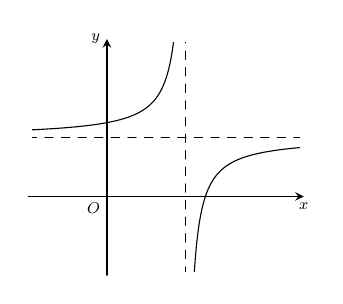
\begin{tikzpicture}[line join = round,line cap = round,>=stealth,font=\footnotesize,scale=0.5]
     \def\xt{-2} \def\xp{5}  \def\yd{-2} \def\yt{4}
     \def\a{6} 
      \def\b{-15}
      \def\c{4}
     \def\d{-8} 
     \draw[->]  (\xt,0)--(\xp,0) node[below]{$x$};
     \draw[->]  (0,\yd)--(0,\yt) node[left]{$y$};
     \fill (0,0) circle (1pt)  node[below left]{$O$};
      \pgfmathsetmacro{\tcn}{(\a)/(\c)}
     \pgfmathsetmacro{\tcd}{-(\d)/(\c)} 
     \begin{scope}
       \clip (\xt+0.1,\yd+0.1) rectangle (\xp-0.1,\yt-0.1);
      \draw[dashed] (\xt,\tcn)--(\xp,\tcn) 
      (\tcd,\yd)--(\tcd,\yt); 
       \draw[samples=150,smooth,domain={\tcd+0.01}:\xp] plot (\x,{(\a*\x+(\b))/(\c*\x+(\d))});
      \draw[samples=150,smooth,domain=\xt:{\tcd-0.01}] plot  (\x,{(\a*\x+(\b))/(\c*\x+(\d))});
     \end{scope}
    \end{tikzpicture}
   \\ 
   Đồ thị $y=f(x)$ &Đồ thị $y=g(x)$&  Đồ thị $y=h(x)$ &Đồ thị $y=k(x)$
  \end{tabular}
 \end{center}
  \choiceTF
  {Hàm số $y=f(x)$ liên tục trên tập xác định của nó} 
  {\True Hàm số $y=g(x)$ liên tục trên tập  xác định của nó}
  {\True  Hàm số $y=h(x)$ không liên tục trên tập xác định của nó}
  {\True Hàm số $y=k(x)$ liên tục trên các khoảng xác định của nó} 
 \loigiai{ 
  Quan sát đồ  thị ta thấy
  \begin{itemize}
   \item Hàm số $y=f(x)$ không liên tục  trên tập xác định (có một điểm gián đoạn).
   \item  Hàm số $y=g(x)$ liên tục trên tập xác định $\mathbb{R}$.
   \item Hàm số $y=h(x)$ không liên tục trên tập  xác định (có một điểm gián đoạn).
   \item Hàm số $y=k(x)$ liên tục  trên các khoảng của tập xác định.
  \end{itemize}
  }
\end{ex}

% từ: cau-hoi/lop11/1D3_Gioi_han_Ham_so_lien_tuc/1D3-3-3_Ham_so_lien_tuc_tai_mot_diem.tex
\begin{ex}%[1D3H3-3]%[ma:99d0e79d]
  Cho hàm số $f\left( x \right)= \heva{& x^{2}+3x, x\geq 2 \\
  & 6x+1 ,x<2 }$. Khi đó
 \choiceTF 
  {$f\left(  2 \right)=13$}
   {\True $\lim\limits_{x\to 2^{+}}f(x)=10$}
  {Tồn tại  $\lim\limits_{x\to 2}f(x)$}
  {\True Hàm số gián đoạn  tại $x=2$}
 \loigiai{ 
  \begin{itemchoice}
   \itemch \textbf{Sai}.\\ 
   $f(2)=2^{2}+3\cdot2=10$. 
   \itemch  \textbf{Đúng}.\\
   $\lim\limits_{x\to 2^{+}}f(x)=\lim\limits_{x\to  2^{+}}(x^{2}+3x)=10$.
   \itemch  \textbf{Sai}.\\
    $\lim\limits_{x\to 2^{+}}f(x)=\lim\limits_{x\to 2^{+}}(x^{2}+3x)=10$ và $\lim\limits_{x\to 2^{-}}f(x)=\lim\limits_{x\to 2^{-}}(6x+1)=13$. \\
   Do đó, không tồn tại $\lim\limits_{x\to 2}f(x)$. 
   \itemch  \textbf{Đúng}.\\
   Vì không tồn tại  $\lim\limits_{x\to 2}f(x)$ nên hàm số gián đoạn tại $x=2$.
  \end{itemchoice}
  }
\end{ex}

% từ: cau-hoi/lop11/1D3_Gioi_han_Ham_so_lien_tuc/1D3-3-5_Bai_toan_phuong_trinh_co_nghiem.tex
\begin{ex}%[1D3H3-5]%[ma:5785ab2b]
	Phương trình $3x^5 + 5x^3 + 10 = 0$ có nghiệm  thuộc khoảng nào sau đây?
	\choice 
		{\True $(-2; -1)$} 
		{$(-10; -2)$} 
		 {$(0; 1)$}
		{$(-1; 0)$} 
	 \loigiai{
		Xét hàm số $f(x) = 3x^5  + 5x^3 + 10$ liên tục trên $\mathbb{R}$.\\
		Suy ra $f(x)$  liên tục trên $[-2; -1]$.\\
		Ta  có
		\[ 
		\heva{ 
		 &f(-2) = -126 \\
		&f(-1) = 2. 
		} 
		 \]
		Suy ra $f(-2) \cdot f(-1) <  0$.\\
		 Do đó $f(x) = 0$ có nghiệm thuộc khoảng $(-2; -1)$.
	 }
\end{ex}

% từ: cau-hoi/lop11/1D3_Gioi_han_Ham_so_lien_tuc/1D3-3-5_Bai_toan_phuong_trinh_co_nghiem.tex
\begin{ex}%[1D3H3-5]%[ma:edb95d0c]
	Chứng minh rằng phương trình $x^3+(m+3)x^2+(1-m)x-1=0$ luôn có nghiệm với mọi  giá trị của $m$.
	\loigiai{ 
		Xét hàm  số $f(x)=x^3+(m+3)x^2+(1-m)x-1$ liên tục trên $\mathbb{R}$ nên cũng liên tục trên khoảng $(0;1)$.\\
		Ta có 
		$\begin{aligned}
		& f(0)=-1 <  0 \\
		& f(1)=4 >  0 .
	\end{aligned}$\\
	Suy ra  $f(0)\cdot f(1)<0$.\\
	Vậy trên  khoảng $(0;1)$ phương trình có ít nhất một nghiệm.
} 
\end{ex}

% từ: cau-hoi/lop11/1D3_Gioi_han_Ham_so_lien_tuc/1D3-3-5_Bai_toan_phuong_trinh_co_nghiem.tex
\begin{ex}%[1D3V3-5]%[ma:97e5eae1]
	Chứng minh rằng phương trình $a\cos 3x+b\cos 2x+c\cos x+\sin x=0$ luôn có nghiệm trên  $[0; 2\pi]$.
	\loigiai{ 
		Xét hàm  số $f(x)=a\cos 3x+b\cos 2x+c\cos x+\sin x$ liên tục trên $\mathbb{R}$.\\
		Nên cũng liên tục trên các đoạn  $[0; 2\pi]$.\\
		$f(0)=a+b+c$, $f\left(\dfrac{\pi}{2}\right)=-b+1$, $f(\pi)=-a+b-c$,  $f\left(\dfrac{3\pi}{2}\right)=-b-1$.\\
		Suy ra $f(0)+f\left(\dfrac{\pi}{2}\right)+f(\pi)+f\left(\dfrac{3\pi}{2}\right)=0$ nên suy  ra nếu không có giá trị nào trong bốn giá trị bằng 0 thì ít nhất có một giá trị âm và dương.\\
		Từ đó suy ra  điều phải chứng minh.
	} 
\end{ex}

% từ: cau-hoi/lop11/1D3_Gioi_han_Ham_so_lien_tuc/1D3-3-5_Bai_toan_phuong_trinh_co_nghiem.tex
\begin{bt}%[1D3V3-5]%[ma:0f3364ea]
% nguon: Archive/SP_KhoLatex/ID6_old/1-CK1-OT-De-14.tex #3510
 
	Chứng minh rằng phương trình $\cos 3x+a\cos 2x+b\cos x+\sin x=0$ luôn có nghiệm với mọi $a, b\in\mathbb{R}$.
	\loigiai{
		Xét hàm số: $f(x)=\cos 3x+a\cos 2x+b\cos x+\sin x$, hàm số liên tục trên $\mathbb{R}$.\\
		Ta có  $f(0)=1+a+b; f\left(\dfrac{\pi}{2}\right)=-a+1; f(\pi)=-1+a-b; f\left(\dfrac{3\pi}{2}\right)=-a-1$. \\
		Suy ra $ f(0)+f\left(\dfrac{\pi}{2}\right)+f(\pi)+f\left(\dfrac{3\pi}{2}\right)=0$.\\
		\textbf{Trường hợp 1.}  $f(0)=f\left(\dfrac{\pi}{2}\right)=f(\pi)=f\left(\dfrac{3\pi}{2}\right)=0$ chứng tỏ $f(x)=0$ có nghiệm nên phương trình đã cho có nghiệm.\\
		\textbf{Trường hợp 2.}  Tồn tại $2$ trong $4$ số $f(0),f\left(\dfrac{\pi}{2}\right),f(\pi),f\left(\dfrac{3\pi}{2}\right)$ trái dấu giả sử $f(0)\cdot f(\pi)<0$.\\
		mà $f(x)=\cos 3x+a\cos 2x+b\cos x+\sin x$ liên tục trên $[0;\pi]$ nên phương trình $f(x)=0$ có ít nhất một nghiệm trên khoảng (0; $\pi$) chứng tỏ $f(x)=0$ có nghiệm nên phương trình đã cho có nghiệm với mọi $a, b\in\mathbb{R}$.}
\end{bt}

% từ: cau-hoi/lop11/1D5_Cac_so_dac_trung_do_xu_the_trung_tam_cho/1D5-2-1_Cau_hoi_ly_thuyet.tex
\begin{ex}%[1D5Y2-1]%[ma:fbcf775a]
	Cho hàm số $f(x)=\left( 2x-3 \right)^{\frac{5}{6}}$. Tính  $f'(2)$
	 \choice
		{$  \dfrac{5}{6} $}
		{\True  $ \dfrac{5}{3} $}
		{$  -\dfrac{5}{6} $}
		{$ -\dfrac{5}{3}  $}
	\loigiai{ 
		Ta có $f'(x)=\dfrac{5}{6} \cdot 2 \cdot \left( 2x-3 \right)^{-\frac{1}{6}}$ suy ra $f'(2)=  \dfrac{5}{3}$.
	} 
\end{ex}

% từ: cau-hoi/lop11/1D6_Ham_so_mu_va_ham_so_logarit/1D6-3-3_Su_bien_thien_va_do_thi_cua_ham_so_mu_logarit.tex
\begin{ex}%[1D6N3-3]%[ma:ac2777f8]
	 \immini{
	Đường cong trong hình bên là đồ thị của hàm  số nào?
	\choice 
		{\True $y=2^x$} 
		{$y=\log_2 x$} 
		 {$y=x^2$}
		{$y=\left(\dfrac{1}{2}\right)^x$} 
		}{ 
		\begin{tikzpicture}[>=stealth]
				\draw[->] (-2.5,0) -- (2.5,0) node[below] {$x$}; 
				\draw[->] (0,-1) -- (0,3)  node[left] {$y$};
				\draw[fill] (0,0) node[below  right]{$O$} circle (1pt);
				\draw (0,1) node[above left]{$1$}; 
				\begin{scope}
					\clip (-2,-0.5) rectangle  (2,3);
					\draw[smooth,samples=200,domain=-2:2.01] plot  (\x,{(2)^(\x)});
				\end{scope}
			\end{tikzpicture}
		} 
	 \loigiai{
		Dựa vào đồ thị ta thấy, đồ thị trên là đồ thị của hàm số mũ có cơ số $a>1$. Trong các phương án chỉ có hàm số $y = 2^x$  thỏa mãn.
	 }
\end{ex}

% từ: cau-hoi/lop11/1D6_Ham_so_mu_va_ham_so_logarit/1D6-3-3_Su_bien_thien_va_do_thi_cua_ham_so_mu_logarit.tex
\begin{ex}%[1D6N3-3]%[ma:ef371a61]
	\immini 
	 {
	 Hàm số nào có đồ thị như đường cong trong hình vẽ bên?
	 \choice
		 {$y=\left(\dfrac{1}{2}\right)^x$}
		{$y=\log_2x$} 
		{\True  $y=2^x$}
		 {$y=\log_{\tfrac{1}{2}}x$}
		 }
		{ 
		\begin{tikzpicture}[>=stealth,line join=round,line cap=round,font=\footnotesize,scale=1]
				\draw[->] (-3,0)--(3,0) node[below]  {$x$};
				\draw[->] (0,-1.5)--(0,3) node[left] {$y$}; 
				\clip  (-3,-1.5) rectangle (3,3);
				\draw[smooth,samples=100,domain=-3:3] plot (\x,{2^(\x)}); 
				\draw[fill] 
					(0,0) circle  (1pt) node[below left] {$O$}
					(1,0) circle (1pt)  node[below] {$1$}
					(0,1)  circle (1pt) node[left] {$1$}
					(0,2) circle (1pt) node[left]  {$2$};
				 \draw[dashed] (1,0)|-(0,2);
			\end{tikzpicture}
		} 
	\loigiai{ 
	Vì đồ thị hàm số luôn nằm trên trục hoành nên đây là  đồ thị của hàm số mũ.\\
	Vì hàm số đồng biến trên $\mathbb{R}$ nên cơ số  phải lớn hơn $1$.\\
	Do đó hàm số cần tìm  là $y=2^x$.
	 }
\end{ex}

% từ: cau-hoi/lop11/1D6_Ham_so_mu_va_ham_so_logarit/1D6-3-3_Su_bien_thien_va_do_thi_cua_ham_so_mu_logarit.tex
\begin{ex}%[1D6H3-3]%[ma:8530d9fd]
	\immini{Đồ thị  hình bên là đồ thị của hàm số nào?
	 \choice
		 {$y=2^x$}
		{$y=\left(\dfrac{1}{2}\right)^x$} 
		 {$y=\left(\dfrac{1}{3}\right)^x$}
		{\True $y=3^x$}}{\begin{tikzpicture}[line join = round,line cap = round,>=stealth,font=\footnotesize,scale =1]
		 \def\a{3}
		\def\f (#1){(\a)^(#1)} 
		 \def\xmin{-3}
		\def\xmax{2} 
		\def\ymin{-1} 
		\def\ymax{4} 
		\draw[->]  (\xmin,0)--(\xmax,0) node[below] {\footnotesize $x$};
		\draw[->] (0,\ymin)--(0,\ymax) node[right] {\footnotesize $y$}; 
		\draw (0,0) node  [below left] {\footnotesize $O$};
		\draw[thick,smooth,samples=200]  plot[domain=\xmin:1.2] (\x,{\f (\x)});
		 \draw[dashed] (1,0)--(1,3)--(0,3);
		\path (1,0) node[below]{$1$} 
			(0,3)  node[left]{$3$};
		\fill (1,3)  circle (1pt);
	\end{tikzpicture}
		} 
	\loigiai{Đồ thị hàm số \lq\lq đi lên\rq\rq~và qua điểm có tọa độ $(1;3)$ nên trong 4 phương án đã cho thì hàm số $y=3^x$  thỏa mãn được tính chất.}
\end{ex}

% từ: cau-hoi/lop11/1D6_Ham_so_mu_va_ham_so_logarit/1D6-3-3_Su_bien_thien_va_do_thi_cua_ham_so_mu_logarit.tex
\begin{ex}%[1D6H3-3]%[ma:657aa4dc]
	Đường cong trong hình bên là của đồ thị hàm số nào sau  đây?
	\begin{center}
		\begin{tikzpicture}[line join=round,line cap=round,>=stealth,scale=0.7]
				 \tikzset{every node/.style={scale=0.9}}
				\draw[->] (-6.1,0)--(6.1,0)  node[below left] {$x$};
				\draw[->] (0,-1.1)--(0,4.1) node[below  left] {$y$};
				\draw (0,0) node  [below left] {$O$};
				\begin{scope}
					\clip (-6,-1)  rectangle (6,4);
					\draw[samples=200,domain=-5.5:5.5,smooth,variable=\x] plot (\x,{0.8^(\x)}); 
				\end{scope}
			\end{tikzpicture}
	\end{center}
	\choice 
		{$y=\log_2x$} 
		{\True  $y=(0{,},8)^x$}
		 {$y=\log_{0{,}4}x$}
		{$y=(\sqrt  2)^x$}
	 \loigiai{
	Dựa vào đồ thị, ta có hàm số có tập xác định $\mathbb{R}$ và hàm  số nghịch biến suy ra $y=(0{,}8)^x$.}
\end{ex}

% từ: cau-hoi/lop11/1D6_Ham_so_mu_va_ham_so_logarit/1D6-3-3_Su_bien_thien_va_do_thi_cua_ham_so_mu_logarit.tex
\begin{ex}%[1D6H3-3]%[ma:7da53078]
	\immini{Đồ thị của hàm số sau là  đồ thị của hàm số nào?
	 \choice
		 {$y=x^2$}
		{$y=3^x$} 
		 {$y=\log_2 x$}
		{\True $y=2^x$}}{\begin{tikzpicture}[line join = round,line cap = round,>=stealth,font=\footnotesize,scale =1]
		 \def\a{2}
		\def\f (#1){(\a)^(#1)} 
		 \def\xmin{-3}
		 \def\xmax{3}
		\def\ymin{-1} 
		 \def\ymax{5}
		\draw[->] (\xmin,0)--(\xmax,0) node[below] {\footnotesize  $x$};
		\draw[->] (0,\ymin)--(0,\ymax) node[right] {\footnotesize $y$}; 
		 \draw (0,0) node [below left] {\footnotesize $O$};
		\draw[thick,smooth,samples=200] plot[domain=\xmin:2.2] (\x,{\f  (\x)});
		\draw[dashed] (2,0)--(2,4)--(0,4); 
		\path  (2,0) node[below]{$2$}
			(0,4)  node[left]{$4$}
			 (0,1) node[above left]{$1$};
		\fill (2,4) circle (1pt) 
			(0,1)  circle (1pt);
	\end{tikzpicture}
		} 
	\loigiai{Nhận thấy đồ thị hàm số đi qua hai điểm $(0;1)$ và  $(2;4)$, đối chiếu với các hàm số ta chọn hàm số $y = 2^x$.}
\end{ex}

% từ: cau-hoi/lop11/1D6_Ham_so_mu_va_ham_so_logarit/1D6-3-3_Su_bien_thien_va_do_thi_cua_ham_so_mu_logarit.tex
\begin{ex}%[1D6H3-3]%[ma:2a93576b]
	\immini{Cho ba số thực dương $a$, $b$, $c$ khác $1$. Đồ thị các hàm số $y=a^x$,  $y=b^x$, $y=c^x$ được cho trong hình vẽ bên. Mệnh đề nào dưới đây đúng?
	\begin{center}
		\begin{tikzpicture}[scale=1,font=\footnotesize,line join=round,line cap=round,>=stealth,x=0.6cm,y=0.6cm,declare function={f (\x)=2^(\x); g (\x)=3^(\x); h (\x)=0.5^(\x);}]
				\def \xmin{-3.0}; 
				\def \xmax{3.5}; 
				\def \ymin{-1.0}; 
				 \def \ymax{5.5};
				\draw[->] (\xmin,0.) -- (\xmax,0.)  node[anchor=north] {$x$};
				 \draw[->] (0.,\ymin) -- (0.,\ymax) node[anchor=west] {$y$};
				\clip  (\xmin+0.1,\ymin+0.1) rectangle (\xmax-0.1,\ymax-0.1);
				\draw[smooth,samples=100,domain=\xmin:\xmax] plot (\x,{f (\x)}) plot (\x,{g (\x)})  plot (\x,{h (\x)});
				 \draw (-2,\ymax) node[right,rotate=-70]{$y=a^x$}
					(1.2,\ymax)  node[left,rotate=80]{$y=b^x$}
					(2.3,\ymax-2)  node[right,rotate=70]{$y=c^x$};
				\foreach \x/\y/\l/\g in {0/0/O/225,0/1/1/180}{\fill[black] (\x,\y)  circle (1pt)+(\g:0.5) node{$\l$};}
			\end{tikzpicture}
	\end{center}
	\choice 
		{$a < b < c$} 
		 {\True $a < c < b$}
		{$b < c <  a$}
		{$c  < a < b$}}{x}
	 \loigiai{
		Từ đồ thị suy ra  $0 < a < 1$;\\
		$b > 1$, $c > 1$ và $b^x>c^x$ khi $x > 0$ nên $b  > c$.\\
		Vậy $a  < c < b$.
	} 
\end{ex}

% từ: cau-hoi/lop11/1D6_Ham_so_mu_va_ham_so_logarit/1D6-3-3_Su_bien_thien_va_do_thi_cua_ham_so_mu_logarit.tex
\begin{ex}%[1D6H3-3]%[ma:3dacb43d]
	Cho hàm số $y=\log_{\tfrac{1}{\mathrm{e}}} x$.  Khẳng định nào sau đây đúng?
	 \choice
		{Hàm số đã cho đồng  biến trên $\mathbb{R}$}
		{Hàm số  đã cho nghịch biến trên $\mathbb{R}$}
		{Hàm số đã cho đồng biến  trên $(0;+\infty)$}
		{\True  Hàm số đã cho nghịch biến trên $(0;+\infty)$}
	\loigiai{ 
		Hàm số $y=\log_{\tfrac{1}{\mathrm{e}}} x$ có $\dfrac{1}{\mathrm{e}}<1$ nên hàm số nghịch biến trên  $(0;+\infty)$.
	} 
\end{ex}

% từ: cau-hoi/lop11/1D6_Ham_so_mu_va_ham_so_logarit/1D6-3-3_Su_bien_thien_va_do_thi_cua_ham_so_mu_logarit.tex
\begin{ex}%[1D6H3-3]%[ma:1ca1c862]
	Mệnh đề nào trong các mệnh đề dưới đây  \textbf{sai}?
	\choice 
		{Hàm số $ y={{\left(\dfrac{2018}{\pi } \right)}^{{x^2}+1}}$ đồng  biến trên $\mathbb{R}$}
		{Hàm số $ y=\log x$ đồng biến  trên $( 0;+\infty)$}
		{\True Hàm  số $ y=\ln( -x)$ nghịch biến trên khoảng $( -\infty;0)$}
		{Hàm số $ y={2^x}$ đồng biến trên  $\mathbb{R}$}
	 \loigiai{
	Hàm số $ y={{\left(\dfrac{2018}{\pi }  \right)}^{{x^2}+1}}$ đồng biến trên $( 0;+\infty)$}
\end{ex}

% từ: cau-hoi/lop11/1D6_Ham_so_mu_va_ham_so_logarit/1D6-3-3_Su_bien_thien_va_do_thi_cua_ham_so_mu_logarit.tex
\begin{ex}%[1D6V3-3]%[ma:77249fd0]
	Cho $a$, $b$ là các số thực dương khác $1$, đường thẳng $d$ song song trục hoành cắt trục tung, đồ thị hàm số $y=a^x$, đồ thị hàm số $y=b^x$ lần lượt tại $H$, $M$, $N$ (như hình  bên). Biết $HM=3MN$. Mệnh đề nào sau đây đúng?
	\begin{center}
		\begin{tikzpicture}[line join=round,line cap=round,>=stealth]
				\tikzset{every  node/.style={scale=0.9}}
				\draw[->] (-1.1,0)--(4.1,0)  node[below left] {$x$};
				\draw[->] (0,-1.1)--(0,4.1)  node[below left] {$y$};
				\draw (0,0) node  [below left] {$O$};
				\foreach \y/\ny in  {1/1}
				\draw[thin]  (1pt,\y)--(-1pt,\y) node [above left] {$\ny$};
				\begin{scope}
					\clip (-1,-1.5) rectangle (5,4.1); 
					\draw[samples=200,domain=-1:1.5,smooth,variable=\x] plot (\x,{2.5^(\x)})  node[right]{$y=a^x$};
					\draw[samples=200,domain=-1:3.3,smooth,variable=\x] plot  (\x,{1.5^(\x)}) node[right]{$y=b^x$};
				\end{scope}
				 \coordinate (O) at (0,0);
				 \coordinate (H) at (0,3);
				 \coordinate (h) at (4,3);
				\path[name path=ax,samples=200,domain=-1:1.5,smooth,variable=\x] plot  (\x,{2.5^(\x)});
				\path[name path=bx,samples=200,domain=-1:3.3,smooth,variable=\x]  plot (\x,{1.5^(\x)});
				\path [name path=Hh]  (H)--(h);
				 \path [name intersections={of=ax and Hh,by={M}}];
				\path [name intersections={of=bx and Hh,by={N}}]; 
				\coordinate (Mx) at  (M|-O);
				\coordinate (Nx) at  (N|-O);
				\draw[dashed] (H)--(N) 
					 (M)--(Mx)
					(N)--(Nx); 
				 \foreach \i/\g in {H/180,M/135,N/135}{\draw[fill=white](\i)
					($(\i)+(\g:3mm)$)  node[scale=1]{$\i$};}
			\end{tikzpicture}
	\end{center}
	\choice 
		{$4a=3b$} 
		{\True $b^4=a^3$} 
		{$b^3=a^4$} 
		{$3a=4b$} 
	\loigiai{ 
		Đường thẳng $d$ cắt đồ thị hàm số  $y=a^x$ tại điểm $M\left(x_M;y_M\right) \Rightarrow y_M=a^{x_M}$.\\
		Đường thẳng  $d$ cắt đồ thị hàm số $y=b^x$ tại điểm $N\left(x_N;y_N\right) \Rightarrow y_N=b^{x_N}$.\\
		Mà $y_M=y_N$  $\Rightarrow a^{x_M}=b^{x_N}$.\\
		Ta có $HM=3MN$ hay $HM=\dfrac{3}{4}HN$.\\ 
		Khi đó $x_M=\dfrac{3}{4}{x_N}\Rightarrow a^{\tfrac{3}{4} x_N}=b^{x_N}\Leftrightarrow a^{\tfrac{3}{4}}=b \Leftrightarrow  a^3=b^4$.
	 }
\end{ex}

% từ: cau-hoi/lop11/1D6_Ham_so_mu_va_ham_so_logarit/1D6-3-3_Su_bien_thien_va_do_thi_cua_ham_so_mu_logarit.tex
\begin{ex}%[1D6V3-3]%[ma:60b98637]
	 Cho đồ thị hàm số $y=f(x)$ dưới đây. Xét tính đúng sai của các khẳng định sau
	\begin{center}
		\begin{tikzpicture}[line join=round,line cap=round,>=stealth,xscale=1.2,yscale=1]
				 \tikzset{every node/.style={scale=0.7}}
				\def\a{-2.5}  \def\c{3.5}
				 \def\b{-1} \def\d{4}
				\def\f{3^(\x)} 
				\begin{scope}
					\clip (\a,\b)  rectangle (\c,\d);
					\draw[samples=200,domain=\a:\c,smooth,variable=\x] plot  (\x,{\f});
				\end{scope}
				\draw[->] (\a,0)--(\c+0.5,0) node[below] {$x$}; 
				\draw[->] (0,\b)--(0,\d+0.5) node[left]  {$y$};
				\draw (0,0) node  [below left] {$O$};
				 \foreach \x/\g in {1/60}
				 \fill[black] (\x,0) circle (1pt) + (\g:2.5mm) node {$\x$};
				\foreach \y/\h in {1/180,3/180} 
				\fill[black]  (0,\y) circle (1pt)+ (\h:2.5mm) node {$\y$};
				\foreach \x/\y  in {1/3}
				\draw[dashed,thin]  (\x,0)--(\x,\y)--(0,\y);
				 \node at (1.8,3.8) {$y=a^x$};
			\end{tikzpicture}
	\end{center}
	\choiceTF 
		{Hàm số đã  cho nghịch biến trên khoảng $(0;1)$}
		 {\True Hàm số cho bởi công thức $y=3^x$}
		{\True Đồ thị hàm số đã cho cắt đường thẳng $y=\dfrac{1}{3}$  tại điểm có hoành độ không âm}
		{Đồ thị hàm số đã cho cắt đường thẳng $y=-x+1$ tại điểm  có hoành độ dương}
	\loigiai{ 
		\begin{itemchoice}
			\itemch Dựa vào đồ thị hàm số ta  thấy hàm số đã cho đồng biến trên $\mathbb{R}$.
			 \itemch Đồ thị hàm số đi qua điểm $(1;3)$ suy ra $a=3$.
			\itemch Phương trình hoành độ giao  điểm của $y=3^x$ và đường thẳng $y=\dfrac{1}{3}$ là
			$$3^x=\dfrac{1}{3}\Leftrightarrow x=-1<0.$$ 
			\itemch Phương trình hoành độ giao điểm của $y=3^x$ và đường thẳng  $y=-x+1$ là $$3^x=-x+1\quad (1)$$
			Ta có hàm số $y=3^x$ đồng biến  trên $\mathbb{R}$ và $3^x>0$,$\forall x\in\mathbb{R}$.\\
			Đường thẳng $y=-x+1$ có hệ  số $a=-1<0$ nên nghịch biến trên $\mathbb{R}$.\\
			Ta lại có $3^0=-0+1$ nên phương trình (1) có nghiệm duy nhất  $x=0$.
		\end{itemchoice}
	 }
\end{ex}

% từ: cau-hoi/lop11/1D6_Ham_so_mu_va_ham_so_logarit/1D6-3-3_Su_bien_thien_va_do_thi_cua_ham_so_mu_logarit.tex
\begin{ex}%[1D6V3-3]%[ma:004831f3]
	Trong hình vẽ bên các đường cong $(C_1)\colon y=a^x$, $(C_2)\colon y=b^x$, $(C_3)\colon y=c^x$ và đường thẳng  $y=4$, $y=8$ tạo thành hình vuông $MNPQ$ có cạnh bằng $4$.
	\begin{center}
		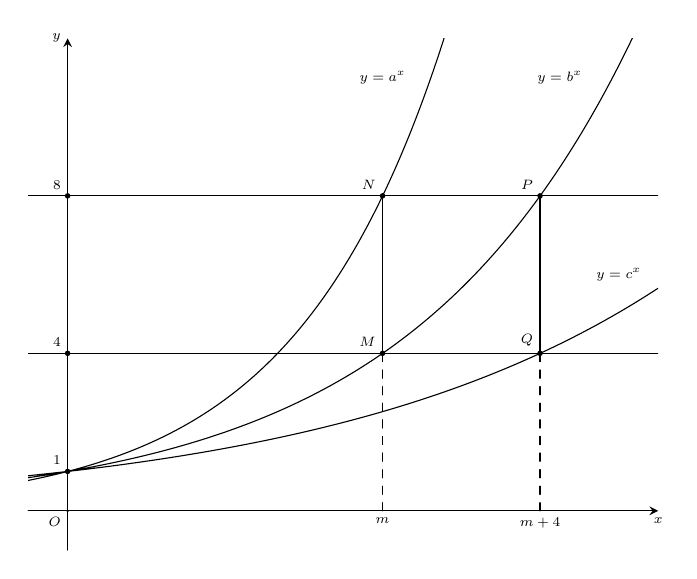
\begin{tikzpicture}[scale=1,>=stealth,font=\scriptsize,line join=round,line cap=round,xscale=.5,yscale=.5]
				\draw[->] (-1,0)--(15,0)  node[below] {$x$};
				\draw[->] (0,-1)--(0,12) node[left] {$y$}; 
				\fill (0,0) circle (1pt) node[below left]{$O$}; 
				 \foreach \x in {8,12}{\fill (\x,4) circle (2pt)
					(\x,8) circle  (2pt);}
				\foreach \y  in {1,4,8}{\fill (0,\y) circle (2pt) node[above left]{$\y$};}
				\clip (-1,-1) rectangle  (15,12);
				 \draw (-1,4)--(15,4);
				\draw (-1,8)--(15,8); 
				 \draw[domain=-2:15,samples=200,smooth]
					plot  (\x,{2^(3/8*\x)})
					 plot (\x,{2^(1/4*\x)})
					plot  (\x,{2^(1/6*\x)});
				\node at (8,11)  {$y=a^x$};
				\node  at (12.5,11) {$y=b^x$};
				\node at  (14,6) {$y=c^x$};
				 \draw[dashed]
					(8,4) node[above left]{$M$}--(8,0) node[below]{$m$} 
					 (12,4) node[above left]{$Q$}--(12,0) node[below]{$m+4$};
				\draw 
					(8,4)--(8,8) node[above  left]{$N$}
					(12,4)--(12,8) node[above  left]{$P$};
			\end{tikzpicture}
	\end{center}
	Biết rằng $abc=2^{\tfrac{x}{y}}$ với $x$, $y\in \mathbb{Z}^+$ và $\dfrac{x}{y}$ tối giản, giá trị của $x+y$ bằng bao nhiêu? 
	\shortans{43} 
	\loigiai{ 
		Giả sử hoành độ $M$ là $m$, ta suy ra $M(m;4)$,  $N(m;8)$, $P(m+4;8)$, $Q(m+4;4)$.\\
		Từ giả thiết ta có $M$, $P$ thuộc đường cong $y=b^x$ nên  $\heva{&b^m=4 \\&b^{m+4}=8}\Leftrightarrow \heva{&b^m=4 \\&b^4=2}\Leftrightarrow \heva{&m=8 \\&b=2^{\tfrac{1}{4}}.}$\\
		Do $N$, $Q$ lần lượt  thuộc cong $y=a^x$ và $y=c^x$ nên $\heva{&a^8=8 \\&c^{12}=4}\Leftrightarrow \heva{&a=2^{\tfrac{3}{8}} \\&c=2^{\tfrac{1}{6}}.}$\\
		 Khi đó $abc=2^{\tfrac{3}{8}}\cdot 2^{\tfrac{1}{4}}\cdot 2^{\tfrac{1}{6}}=2^{\tfrac{3}{8}+\tfrac{1}{4}+\tfrac{1}{6}}=2^{\tfrac{19}{24}}$.\\
		Suy ra $x=19$ và  $y=24$.\\
		Vậy $x+y=43$. 
	 }
\end{ex}

% từ: cau-hoi/lop11/1D6_Ham_so_mu_va_ham_so_logarit/1D6-3-4_So_sanh_cac_luy_thua_va_logarit.tex
\begin{ex}%[1D6H3-4]%[ma:943f499b]
	Cho số  thực $a$ thỏa $a>1$. Mệnh đề nào sau đây \textbf{đúng}?
	 \choice
		{$\sqrt[3]{a^2}>a$} 
		{\True  $a^{-\sqrt{3}}>\dfrac{1}{a^{\sqrt{5}}}$}
		 {$a^{\frac{1}{3}}>\sqrt{a}$}
		 {$\dfrac{1}{a^{2023}}<\dfrac{1}{a^{2024}}$}
	\loigiai{ 
		Ta  có
		\begin{itemize}
			\item  Xét đáp án $\sqrt[3]{a^2}>a$. Vì $\dfrac{2}{3}<1$ nên $\sqrt[3]{a^2}<a$.
			\item Xét đáp án $a^{-\sqrt{3}}>\dfrac{1}{a^{\sqrt{5}}}$. Vì $-\sqrt{3}>-\sqrt{5}$ nên  $a^{-\sqrt{3}}>\dfrac{1}{a^{\sqrt{5}}}$.
			\item  Xét đáp án $a^{\frac{1}{3}}>\sqrt{a}$. Vì $\dfrac{1}{3}<\dfrac{1}{2}$ nên $a^{\frac{1}{3}}<\sqrt{a}$.
			\item Xét đáp án $\dfrac{1}{a^{2023}}<\dfrac{1}{a^{2024}}$. Vì $\dfrac{1}{2023}>\dfrac{1}{2024}$  nên $\dfrac{1}{a^{2023}}<\dfrac{1}{a^{2024}}$.
		\end{itemize}
	 }
\end{ex}

% từ: cau-hoi/lop11/1D6_Ham_so_mu_va_ham_so_logarit/1D6-3-4_So_sanh_cac_luy_thua_va_logarit.tex
\begin{ex}%[1D6V3-4]%[ma:6b5f59ff]
	Cho $a$, $b$ là các số thực dương khác $1$, đường thẳng $d$ song song trục hoành cắt trục tung, đồ thị hàm số $y=a^x$, đồ thị hàm số $y=b^x$ lần lượt tại $H$, $M$, $N$. Biết $HM=3MN$. Mệnh đề nào sau đây đúng? 
	\begin{center}
		\begin{tikzpicture}[line join = round,line cap = round,>=stealth,font=\footnotesize,scale =1]
				\draw[->] (-2,0)--(0,0) node[below right]{$O$}--(4.5,0) node[below]{$x$}; 
				\draw[->] (0,-1)--(0,4.5)  node[right]{$y$};
				\draw (-2,2)--(4.5,2)  node [right]{$d$};
				\clip  (-2,-1) rectangle (3,4.5);
				\draw[samples=300,domain=-2.5:4.5,smooth] plot (\x,{(2)^(\x)}); 
				\draw[samples=300,domain=-2.5:4.5,smooth]  plot (\x,{(1.68)^(\x)});
				 \path[name path=ab] (-2,2)--(4.5,2);
				\path[name path=f] plot (\x,{(2)^(\x)}); 
				\path[name path=g] plot (\x,{(1.68)^(\x)}); 
				\coordinate (H)  at (0,2);
				\path[name intersections={of= ab  and f,by=M}];
				 \path[name intersections={of= ab and g,by=N}];
				 \coordinate (E) at ($(0,0)!(M)!(4,0)$);
				\coordinate (F) at ($(0,0)!(N)!(4,0)$); 
				\foreach \x/\y in {M/above left,N/below right,H/below left} \fill (\x) node [\y] {$\x$}  circle (1pt);
				 \fill (E) node [below] {$x_M$} circle (1pt);
				\fill (F) node [below right]  {$x_N$} circle (1pt);
				\draw[dashed] (M)--(E) 
					(N)--(F); 
			\end{tikzpicture}
	\end{center}
	 \choice
		{$4a=3b$} 
		 {\True $b^4=a^3$}
		{$b^3=a^4$} 
		 {$3a=4b$}
	 \loigiai{
		Đường thẳng $d$ cắt đồ thị hàm số $ y=a^x$ tại điểm  $ M(x_M;y_M)$ $\Rightarrow{y_M}=a^{x_M}$.\\
		Đường thẳng $ d$ cắt  đồ thị hàm số $ y=b^x$ tại điểm $ N(x_N;y_N)$ $\Rightarrow{y_N}=b^{x_N}$.\\
		 Mà $y_M=y_N$ $\Rightarrow{a^{x_M}}=b^{x_N}$.\\
	Ta có $  HM=3MN$ $\Rightarrow HM=\dfrac{3}{4}HN$ $\Rightarrow{x_M}=\dfrac{3}{4}{x_N}$ $\Rightarrow{a^{\tfrac{3}{4}{x_N}}}=b^{x_N}$ $\Leftrightarrow{a^{\tfrac{3}{4}}}=b$ $\Leftrightarrow{a^3}=b^4$.}
\end{ex}

% từ: cau-hoi/lop11/1D6_Ham_so_mu_va_ham_so_logarit/1D6-4-3_Bat_phuong_trinh_mu_logarit_co_ban.tex
\begin{ex}%[1D6V4-3]%[ma:c454180e]
	Có bao nhiêu số nguyên $x$ thỏa mãn $(-\log _2^2 x+5\log _2 x+6)\cdot\sqrt{3-\log _5  x} \ge 0$?
	 \shortans{65}
	 \loigiai{
		Điều  kiện $\heva{&x>0\\&3-\log _5 x\ge 0} \Leftrightarrow \heva{&x>0\\&\log _5 x\le 3} \Leftrightarrow \heva{&x>0\\&x\le 125} \Leftrightarrow 0<x\le 125$.\\
		Xét hàm số $f(x)=(-\log _2^2 x+5\log _2 x+6)\cdot\sqrt{3-\log _5 x} $, khi đó $f(x)$ là  hàm số xác định và liên tục trên $(0;125]$.\\
		Ta có $f(x)=0\Leftrightarrow \hoac{&-\log _2^2  x+5\log _2 x+6=0 &(1)\\&\sqrt{3-\log _5 x} =0. &(2)} $\\
		Phương trình tương đương $\hoac{&\log _2 x=-1\\&\log _2 x=6} \Leftrightarrow \hoac{&x=\dfrac{1}{2}\\&x=64.}  $\\
		Phương trình tương  đương $\log _5 x=3\Leftrightarrow x=125$.\\
		Ta có bảng xét  dấu như sau
		\begin{center}
			
\begin{tikzpicture}
					 \tkzTabInit[nocadre=false,lgt=2,espcl=2,deltacl=0.5]
						 {$x$/1,$f (x)$/1}
						 {$0$,$\dfrac{1}{2}$,$64$,$125$}
					\tkzTabLine{d,-,z,+,z,-,z} 
				\end{tikzpicture}
		\end{center}
		Vậy tập nghiệm của bất phương  trình là $S=\left[\dfrac{1}{2};64\right]\cup \{125\}$.\\
	Do đó có  $65$ số nguyên $x$.}
\end{ex}

% từ: cau-hoi/lop11/1D6_Ham_so_mu_va_ham_so_logarit/1D6-4-3_Bat_phuong_trinh_mu_logarit_co_ban.tex
\begin{bt}%[1D6N4-3]%[ma:1d7b6677]
% nguon: Archive/2024/TOAN_11_XE/TOAN_11_XE/data4/11C6/KNTT-6.4.tex #1017
%[TeX hóa SGK 11 - CTST - Đoàn Mạnh Hùng]
	Giải các bất phương trình sau
	\begin{listEX}[3]
		\item $10^x<0{,}001$.
		\item $0{,}4^x>2$.
		\item $\left(\dfrac{1}{2}\right)^x \geq 2 \cdot 4^{2x}$.
	\end{listEX}
	\loigiai{
		\begin{listEX}[1]
			\item $10^x<0{,}001 \Leftrightarrow 10^x<10^{-3} \Leftrightarrow x<-3$ (do $10>1$ ).
			\item $0{,}4^x>2 \Leftrightarrow x<\log _{0{,}4} 2$ (do $0<0{,}4<1)$.
			\item
			\allowdisplaybreaks
			\begin{eqnarray*}
				&&\left(\dfrac{1}{2}\right)^x \geq 2 \cdot 4^{2 x}  \Leftrightarrow\left(2^{-1}\right)^x \geq 2 \cdot\left(2^2\right)^{2 x} \Leftrightarrow 2^x \geq 2^{1+4 x} \\
				&\Leftrightarrow&-x \geq 1+4 x \Leftrightarrow 5 x \leq-1 \Leftrightarrow x \leq-\dfrac{1}{5}.
			\end{eqnarray*}
		\end{listEX}
	}
\end{bt}

% từ: cau-hoi/lop11/1D6_Ham_so_mu_va_ham_so_logarit/1D6-4-3_Bat_phuong_trinh_mu_logarit_co_ban.tex
\begin{bt}%[1D6N4-3]%[ma:225d92ab]
% nguon: Archive/2024/TOAN_11_XE/TOAN_11_XE/data4/11C6/KNTT-6.4.tex #1018
%[TeX hóa SGK 11 - CTST - Đoàn Mạnh Hùng]
	Giải các bất phương trình sau
	\begin{listEX}[3]
		\item $2^x>16$.
		\item $0{,}1^x \leq 0{,}001$.
		\item $\left(\dfrac{1}{5}\right)^{x-2} \geq\left(\dfrac{1}{25}\right)^x$.
	\end{listEX}
	\loigiai{
		\begin{listEX}[1]
			\item $2^x>16\Leftrightarrow x>4$.
			\item $0{,}1^x \leqslant  0{,}001\Leftrightarrow 0{,}1^x \leqslant  0{,}1^3\Leftrightarrow x\geqslant 3$.
			\item $\left(\dfrac{1}{5}\right)^{x-2} \geqslant \left(\dfrac{1}{25}\right)^x\Leftrightarrow \left(\dfrac{1}{5}\right)^{x-2}\geqslant \left(\dfrac{1}{5}\right)^{2x}\Leftrightarrow x-2\leqslant 2x\Leftrightarrow x\geqslant -2$.
		\end{listEX}
	}
\end{bt}

% từ: cau-hoi/lop11/1D6_Ham_so_mu_va_ham_so_logarit/1D6-4-5_Bat_phuong_trinh_mu_logarit_dua_ve_cung_co_so.tex
\begin{ex}%[1D6H4-5]%[ma:58cce9a6]
	Giải các bất phương  trình sau
	\begin{listEX}[2]
		\item $2^{2x-1}-2^{-2}>0$; 
		\item  $2^{2(x+5)^2} \ge 4^{1-2x}$.
	\end{listEX}
	\loigiai{ 
		\begin{listEX}
			\item Ta có $2^{2x-1}-2^{-2}>0 \Leftrightarrow 2^{2x-1}>2^{-2}  \Leftrightarrow 2x-1>-2 \Leftrightarrow x>-\dfrac{1}{2}$.\\
			Vậy  tập nghiệm của bất phương trình là $S=\left(-\dfrac{1}{2};+\infty\right)$.
			\item  Ta có
			\begin{eqnarray*}
				2^{2(x+5)^2} \ge  4^{1-2x}
				&\Leftrightarrow& 4^{(x+5)^2} \ge 4^{1-2x}\\ 
				&\Leftrightarrow& (x+5)^2 \ge  1-2x \\
				&\Leftrightarrow& x^2+4x+24 \ge 0 \\ 
				&\Leftrightarrow&  (x+2)^2+20>0, \ \forall x \in \mathbb{R}.
			\end{eqnarray*}
			Vậy  tập nghiệm của bất phương trình là $S=\mathbb{R}$.
		\end{listEX}
	} 
\end{ex}

% từ: cau-hoi/lop11/1D6_Ham_so_mu_va_ham_so_logarit/1D6-4-5_Bat_phuong_trinh_mu_logarit_dua_ve_cung_co_so.tex
\begin{ex}%[1D6H4-5]%[ma:8c451cf0]
	Giải các bất phương trình  sau
	\begin{listEX}[2]
		\item $2^{x+1}>8^{x-1}$; 
		 \item $3^{4^x} \le 4^{3^x}$.
	\end{listEX}
	\loigiai{ 
		\begin{listEX}
			\item Ta có \begin{eqnarray*}
			2^{x+1}>8^{x-1} 
			&\Leftrightarrow& x+1>(x-1)\log_2 8\\ 
			&\Leftrightarrow&  x+1>3(x-1)\\
			 &\Leftrightarrow& x<-2.
		\end{eqnarray*}
		Vậy tập nghiệm của bất  phương trình là $S=\left(-\infty;-2\right)$.
		\item Ta có \begin{eqnarray*}
		3^{4^x}  \le 4^{3^x}
		&\Leftrightarrow& 4^x \log_3 3 \le 3^x  \log_3 4\\
		&\Leftrightarrow& \left(\dfrac{4}{3}\right)^x \le \log_3 4\\ 
		&\Leftrightarrow& x \le  \log_{\tfrac{4}{3}}\left(\log_3 4\right).
	\end{eqnarray*}
	Vậy tập nghiệm của bất  phương trình là $S=\left(-\infty;\log_{\tfrac{4}{3}}\left(\log_3 4\right)\right]$.
	\end{listEX}
} 
\end{ex}

% từ: cau-hoi/lop11/1D7_Dao_ham/1D7-1-5_Toan_thuc_te_khac_ap_dung_dinh_nghia_dao_ham.tex
\begin{ex}%[1D7V1-5]%[ma:c76dd2b2]
	Người ta xây dựng một cây cầu vượt giao thông hình parabol nối hai điểm có khoảng cách là $400$\,m. Độ dốc của mặt cầu không vượt quá $10^\circ$ (độ dốc tại một điểm được xác định bởi góc giữa phương tiếp xúc với mặt cầu và  phương ngang). Chiều cao giới hạn từ đỉnh cầu đến mặt đường là bao nhiêu mét? (làm tròn kết quả đến chũ số thập phân thứ nhất).
	\begin{center}
		\begin{tikzpicture}[line cap=butt,line join=miter,>=stealth,font=\normalsize]
				\path (-3.5,-49/48) coordinate (P) 
					(-2.5,-49/48) coordinate (Q) 
					(-2.5,-7/16) coordinate (R); 
				\tikzset{declare  function={xmin=-6; xmax=6; ymin=-3; ymax=0;
					f (\x)=-1/12*(\x)^2; 
					g  (\x)=7/12*(\x)+49/48;
					}, 
					smooth,samples=450 
				} 
				\draw (-6,-3) circle (1pt)  node[left]{$A$}--(6,-3) circle (1pt) node[right]{$B$}
					(-3.5,-49/48) circle (1pt) node[above left]{$P$}; 
				 \draw[dashed](0,0)--(0,-3) node[midway,right]{$h=?$}
					(-3.5,-49/48)--(-2.5,-49/48); 
				\clip (xmin,ymin) rectangle (xmax,ymax); 
				\draw  plot[domain=xmin:xmax] (\x,{f (\x)});
				\draw plot[domain=-4.5:-2.5] (\x,{g  (\x)});
				\draw pic[draw,,angle  radius=4mm]{angle=Q--P--R}
					pic[draw=none,"$10^\circ$",angle radius=12mm,font=\scriptsize]{angle=Q--P--R}; 
			\end{tikzpicture}
	\end{center}
	\shortans{17,6} 
	\loigiai{ 
		\begin{center}
			\begin{tikzpicture}[line cap=butt,line join=miter,>=stealth,font=\normalsize]
					 \path (-3.5,-49/48) coordinate (P)
						(-2.5,-49/48) coordinate (Q) 
						 (-2.5,-7/16) coordinate (R);
					 \tikzset{declare function={xmin=-7; xmax=7; ymin=-4; ymax=1.5;
						f (\x)=-1/12*(\x)^2; 
						g (\x)=7/12*(\x)+49/48; 
						}, 
						 smooth,samples=450
					} 
					\draw[dashed](-6,0)  node[above]{$-200$}|-(0,-3) node[below left]{$I$}
						(6,0)  node[above]{$200$}|-(0,-3)
						 (-3.5,-49/48)--(-2.5,-49/48);
					\draw (-3.5,-49/48) circle (1pt) node[above  left]{$P$}
						(-6,-3)  circle (1pt) node[left]{$A$}
						(6,-3)  circle (1pt) node[right]{$B$};
					\draw[->] (xmin,0)--(xmax,0) node[shift={(-100:7pt)}]{$  x $};
					\draw[->] (0,ymin)--(0,ymax) node[shift={(190:7pt)}]{$ y $}; 
					\fill (0,0) node[shift={(135:10pt)}]{$ O $}; 
					\clip (xmin,ymin) rectangle  (xmax,ymax);
					\draw  plot[domain=-6:6] (\x,{f (\x)});
					\draw  plot[domain=-4.5:-2.5] (\x,{g (\x)});
					\draw  pic[draw,,angle radius=4mm]{angle=Q--P--R}
						pic[draw=none,"$10^\circ$",angle  radius=12mm,font=\scriptsize]{angle=Q--P--R};
				\end{tikzpicture}
		\end{center}
		Chọn hệ trục toạ độ  như hình vẽ, sao cho đỉnh cầu là gốc tọa độ và mặt cắt của cây cầu có hình dạng parabol $(P)\colon y=-ax^2$ (với $a$ là hằng số dương).\\
		Giả sử điểm $P\in (P)$ có hoành độ  $x_0$, với $-200<x_0<200$.\\
		Hệ số góc của tiếp tuyến  của parabol bằng $k=y' \left(x_0 \right)=-2ax_0$.\\
		Hệ số góc xác định độ dốc của mặt cầu (độ dốc dương) là  $\left|k\right|=2a\left|x_0\right|\le 400a$.\\
		Vì độ dốc của  mặt cầu không vượt quá $10^\circ$ nên ta có
		\[400a\le \tan 10^\circ\Leftrightarrow a\le  \dfrac{\tan 10^\circ}{400}.
		 \]
		Chiều cao giới hạn từ đỉnh cầu  đến mặt đường là đoạn $OI$, cũng chính là độ lớn của tung độ điểm $B$ khi $a$ đạt giá trị lớn nhất.\\
		Do đó $OI=\left|-a\cdot 200^2\right|=17{,}6$\,m.\\ 
		Vậy chiều cao giới hạn  từ đỉnh cầu đến mặt đường là $17{,}6$\,m.
	 }
\end{ex}

% từ: cau-hoi/lop11/1D7_Dao_ham/1D7-2-1_Tinh_dao_ham.tex
\begin{ex}%[1D7H2-1]%[ma:6b6e9627]
	Cho hàm  số $f(x)=\sin2x$. Khi đó giá trị $f'\left(\dfrac{\pi}{4}\right)$ bằng
	\choice 
		{$-1$} 
		{\True  $0$}
		{$1$} 
		 {$2$}
	\loigiai{Ta  có $f'(x)=2\cos2x\Rightarrow f'\left(\dfrac{\pi}{4}\right)=2\cos\left(2\cdot\dfrac{\pi}{4}\right)=2\cos\dfrac{\pi}{2}=0$.}
\end{ex}

% từ: cau-hoi/lop11/1D7_Dao_ham/1D7-2-1_Tinh_dao_ham.tex
\begin{ex}%[1D7H2-1]%[ma:cf18e790]
  Tính được đạo hàm của các hàm số sau. Khi đó
 \choiceTF 
  {$y=2\sin x-3\cos x$ có $y'=2\cos x-3\sin  x$}
  {\True  $y=2\cot x-\tan x$ có $y'=-\dfrac{2}{\sin^2 x}-\dfrac{1}{\cos^2 x}$}
  {$y=x\cos  x$ có $y'=\cos x+x\sin x$}
  {\True $y=2x\sin^2 x$ có  $y'=2\sin^2 x+2x\sin x$}
 \loigiai{ 
  \begin{itemize}
   \item $y'=2(\sin x)'-3(\cos x)' =2\cos x+3\sin  x$.
   \item $y'=2(\cot  x)'-(\tan x)' =-\dfrac{2}{\sin^2 x}-\dfrac{1}{\cos^2 x}$.
   \item $y'=x'\cos  x+x (\cos x)'= \cos x-x\sin x.$
   \item 
   \begin{eqnarray*}
     y'&=&(2x)'\sin^2 x+2x(\sin^2 x)'\\
    &=&2\sin^2 x+2x \cdot 2\sin x.(\sin  x)'\\
    &=& 2\sin ^2 x+4x\sin x  \cos x\\
    &=& 2\sin^2  x+2x\sin 2x.
   \end{eqnarray*}
  \end{itemize}
 } 
\end{ex}

% từ: cau-hoi/lop11/1D7_Dao_ham/1D7-2-1_Tinh_dao_ham.tex
\begin{bt}%[1D7V2-1]%[ma:0fe0d4b8]
% nguon: Archive/SP_KhoLatex/ID6_old/16-OT-DaoHam-CongThucTinhDaoHam.tex #3821
%[ĐGNL-Nguyễn Thành Nhân]
	Cho hàm số $y=3x+\sqrt{10-x^2}$. Giải phương trình $y'=0$.
	\loigiai{
		Điều kiện $-\sqrt{10}\leq x\leq \sqrt{10}\quad (*)$.\\
		Ta có $y'=3-\dfrac{x}{\sqrt{10-x^2}}$.\\
		Khi đó, 
		\begin{eqnarray*}
			y'=0 &\Leftrightarrow & 3-\dfrac{x}{\sqrt{10-x^2}}=0\\
			&\Leftrightarrow & 3=\dfrac{x}{\sqrt{10-x^2}}\\ &\Leftrightarrow &3\sqrt{10-x^2}=x\\
			&\Leftrightarrow &  \heva{&x \geq 0\\
				&9\left(10-x^2\right)=x^2}\\
			&\Leftrightarrow & \heva{
				&x \geq 0\\
				&10x^2-90=0}\\
			&\Leftrightarrow & \heva{ &x \geq 0\\
				&x=\pm3} \Leftrightarrow x=3 \quad (\text{thỏa điều kiện}\ (*)).
		\end{eqnarray*}
		Vậy phương trình $y'=0$ có duy nhất nghiệm $x=3$.
	}
\end{bt}

% từ: cau-hoi/lop11/1D7_Dao_ham/1D7-2-1_Tinh_dao_ham.tex
\begin{bt}%[1D7V2-1]%[ma:0521a739]
% nguon: Archive/SP_KhoLatex/ID6_old/16-OT-DaoHam-CongThucTinhDaoHam.tex #3828
%[ĐGNL, Nguyễn Thành Nhân]
Cho hàm số $f(x)=\dfrac{\cos^2 x}{1+\sin^2 x}$. Chứng minh $f\left(\dfrac{\pi}{4}\right)-3f'\left(\dfrac{\pi}{4}\right)=3$.
	\loigiai
	{
		Ta có
		\begin{align*}
		f'(x) &=\dfrac{-2\cos x\sin x\left(1+\sin^2 x\right)-\cos^2 x\cdot 2\sin x\cos x}{\left(1+\sin^2 x\right)^2} = \dfrac{-2\sin x\cos x\left(1+\sin^2 x+\cos^2 x\right)}{\left(1+\sin^2 x\right)^2}\\
		&=-\dfrac{2\sin 2x}{\left(1+\sin^2 x\right)^2}.
		\end{align*}
		Lại có $f\left(\dfrac{\pi}{4}\right)=\dfrac{1}{3}$, $f'\left(\dfrac{\pi}{4}\right)=-\dfrac{8}{9}$.\\
		Do đó
		\[f\left(\dfrac{\pi}{4}\right)-3f'\left(\dfrac{\pi}{4}\right) = \dfrac{1}{3}-3\cdot \left(-\dfrac{8}{9}\right) = 3.\]
	}
\end{bt}

% từ: cau-hoi/lop11/1D7_Dao_ham/1D7-2-8_Toan_thuc_te_ap_dung_quy_tac_dao_ham.tex
\begin{ex}%[1D7H2-8]%[ma:ed9e0b6d]
 Phương trình chuyển động của một hạt được cho bởi công thức $s(t)=10+\sqrt{2}\sin\left(\dfrac{\pi}{4}+4\pi t\right)$, trong đó  $s$ tính bằng centimet và $t$ được tính bằng giây. Xét tính đúng sai của các mệnh đề sau
  \choiceTF
  {Gia tốc của hạt tại  thời điểm $t=3$ giây là $-16\pi^2$ cm/s$^2$}
  {\True Vận tốc của hạt tại  thời điểm $t=3$ giây là $2\pi$ cm/s}
  {\True Vận tốc lớn nhất của hạt đạt được  là $4\pi\sqrt{2}$ cm/s}
  {Gia tốc nhỏ nhất của hạt đạt được là $-16\pi^2$  cm/s$^2$}
 \loigiai{ 
  Ta  có\\
   Vận tốc của hạt tại thời điểm $t$ là $v(t)=s'(t)=4\pi \sqrt{2}\cos\left(\dfrac{\pi}{4}+4\pi t\right)$.\\
  Gia tốc của hạt tại thời điểm $t$ là $a(t)=s''(t)=-16\pi ^2\sqrt{2}\sin\left(\dfrac{\pi}{4}+4\pi t\right)$. 
  \begin{itemchoice}
   \itemch Sai. Tại thời điểm $t=3$ giây thì gia  tốc của hạt là $$a=-16\pi^2\sqrt{2}\sin\left(\dfrac{\pi}{4}+12\pi \right)=-8\pi^2\text{ cm/s}^2.$$
   \itemch Đúng. Tại thời điểm $t=3$ giây thì vận  tốc của hạt là $$v=4\pi\sqrt{2}\cos\left(\dfrac{\pi}{4}+4\pi\cdot 3\right)=2\pi \text{ cm/s.}$$
   \itemch Đúng. Ta  có $-4\pi\sqrt{2}\leq 4\pi\sqrt{2}\cos\left(\dfrac{\pi}{4}+4\pi t\right)\leq 4\pi\sqrt{2}$ nên vận tốc lớn nhất của hạt đạt được là $4\pi\sqrt{2}$ cm/s.
   \itemch  Sai. Ta có $-16\pi^2\sqrt{2}\leq -16\pi^2\sqrt{2}\sin\left(\dfrac{\pi}{4}+4\pi t\right)\leq 16\pi^2\sqrt{2}$ nên gia tốc nhỏ nhất của hạt đạt được là $-16\pi^2\sqrt{2}$ cm/s$^2$.
  \end{itemchoice}
  }
\end{ex}

% từ: cau-hoi/lop11/1D7_Dao_ham/1D7-2-8_Toan_thuc_te_ap_dung_quy_tac_dao_ham.tex
\begin{ex}%[1D7H2-8]%[ma:813cb0c5]
	Cho một vật chuyển động theo phương trình $s(t)=t^2+mt+10$. Trong đó $ s $ là quãng đường vật đi được (mét) và $ t $ là thời gian vật chuyển động (giây). Xác định giá trị của tham số m biết tại thời điểm $t=3$ thì vận tốc  tức thời của vật là $ 4{,}5 $ m/s.
	 \shortans{-1,5}
	\loigiai{ 
		Vận tốc của vật tại thời điểm $ t $ là $v(t)=s'(t)=2t+m$  .\\
	Vận tốc tức thời của vật là  $ 4{,}5 $ m/s khi $v(3)=4{,}5\Leftrightarrow 2\cdot 3+m=4{,}5\Leftrightarrow m=-1{,}5$.}
\end{ex}

% từ: cau-hoi/lop11/1D7_Dao_ham/1D7-2-8_Toan_thuc_te_ap_dung_quy_tac_dao_ham.tex
\begin{ex}%[1D7H2-8]%[ma:9354b609]
	Một chất điểm chuyển  động theo phương trình $s(t)=10+t+9t^2-t^3$ trong đó $s$ tính bằng mét, $t$ tính bằng giây. Tính thời gian để vận tốc của chất điểm đạt giá trị lớn nhất (tính từ thời điểm ban đầu)?
	 \shortans{1,5}
	 \loigiai{
	Ta có $v(t)=s'(t)=-3t^2+9t+1$ có đồ thị là Parabol, do đó $v(t)_{\max}\Leftrightarrow  t=\dfrac{-9}{-6}=\dfrac{3}{2}$.}
\end{ex}

% từ: cau-hoi/lop11/1D9_Xac_suat/1D9-2-4_Quy_tac_cong_cho_hai_bien_co_bat_ki.tex
\begin{ex}%[1D9C2-4]%[ma:7a2991ce]
% nguon: Archive/2024/Update-SP-BG10-11-3/SP-3/BG11-3/data_1C5/DeOT-ChuongV-DeOnTap-So1-VuNguyenHoangAnh.tex #1581

	Có $3$ xạ thủ cùng bắn vào bia với xác suất bắn trúng bia của mỗi xạ thủ lần lượt là $0{,}7$; $0{,}6$ và $0{,}5$.
	\choiceTF[t]
	{\True Xác suất để xạ thủ thứ nhất không bắn trúng bia là $0{,}3$}
	{Xác suất để cả ba xạ thủ bắn trúng bia là $0{,}2$}
	{\True Xác suất để hai xạ thủ thứ nhất và thứ hai bắn trúng còn xạ thủ thứ ba bắn trượt là $0{,}21$}
	{\True Xác suất để có ít nhất hai xạ thủ bắn trúng bia là $0{,}65$}
	\loigiai{
		Gọi $A$, $B$, $C$ lần lượt là xác suất bắn trúng của xạ thủ thứ nhất, thứ hai và thứ ba.
		\begin{itemchoice}
			\itemch Xác suất xạ thủ thứ nhất không bắn trúng là $\mathrm{P}\left(\overline{A}\right)=1-0{,}7=0{,}3$.
			\itemch Xác suất cả ba xạ thủ bắn trúng bia là \[\mathrm{P}\left(ABC\right)=\mathrm{P}(A)\mathrm{P}(B)\mathrm{P}(C)=0{,}7\times 0{,}6\times 0{,}5=0{,}21.\]
			\itemch Xác suất cần tìm là
			\[ \mathrm{P}\left(AB\overline{C}\right)=\mathrm{P}(A)\mathrm{P}(B)\mathrm{P}(\overline{C})=0{,}7\times 0{,}6\times 0{,}5=0{,}21. \]
			\itemch Có ít nhất hai xạ thủ bắn trúng bia khi có đúng hai xạ thủ bắn trúng hoặc cả ba xạ thủ bắn trúng bia. Do đó xác suất cần tìm là
			\begin{align*}
				&\mathrm{P}\left(AB\overline{C}\right)+\mathrm{P}\left(A\overline{B}C\right)+\mathrm{P}\left(\overline{A}BC\right)+\mathrm{P}\left(ABC\right)\\
				=\ &0{,}7\times 0{,}6\times 0{,}5+0{,}7\times 0{,}4\times 0{,}5+0{,}3\times 0{,}6\times 0{,}5+0{,}7\times 0{,}6\times 0{,}5\\
				=\ &0{,}65.
			\end{align*}
		\end{itemchoice} 
	}
\end{ex}

% từ: cau-hoi/lop11/1D9_Xac_suat/1D9-2-5_Tinh_xac_suat_bien_co_hop_bang_so_do_hinh_cay.tex
\begin{bt}%[1D9V2-5]%[ma:a58af999]
% nguon: Archive/2024/Update-SP-BG10-11-3/SP-3/BG11-3/data_1C5/DS11-C5-B2-Dang6-SoDoHinhCay-TranTony.tex #1499
%[Bài giảng 11, Trần Tony]
	Ba xạ thủ cùng bắn, mỗi người một viên đạn vào bia một cách độc lập với nhau. Xác suất bắn trúng bia của ba xạ thủ lần lượt là $\dfrac{1}{2}; \dfrac{1}{4}$ và $\dfrac{1}{3}$. Tính xác suất của biến cố có ít nhất hai xạ thủ không bắn trúng bia (kết quả làm tròn tới hàng phần trăm).
	\shortans{$0{,}86$}
	\loigiai
	{
	Giả sử $A:$\lq\lq Xạ thủ $1$ bắn trúng bia \rq\rq.\\
	Suy ra $\mathrm{P}(A)=\dfrac{1}{2}\Rightarrow \mathrm{P}(\overline{A})=1-\mathrm{P}(A)=1-\dfrac{1}{2}=\dfrac{1}{2}$.\\
	Giả sử $B:$\lq\lq Xạ thủ hai bắn trúng bia \rq\rq.\\
	Suy ra $\mathrm{P}(B)=\dfrac{1}{4}\Rightarrow \mathrm{P}(\overline{B})=1-\mathrm{P}(B)=1-\dfrac{1}{4}=\dfrac{3}{4}$.\\
	Giả sử $C:$ \lq\lq Xạ thủ ba bắn trúng bia \rq\rq.\\
	Suy ra $\mathrm{P}(C)=\dfrac{1}{3}\Rightarrow \mathrm{P}(\overline{C})=1-\mathrm{P}(C)=1-\dfrac{1}{3}=\dfrac{2}{3}$.\\
	Nhận thấy $A, B, C$ là các biến cố độc lập nên suy ra $A, B, C, \overline{A}, \overline{B},\overline{C}$ đôi một độc lập với nhau.\\
	Ta có sơ đồ sau
	\begin{center}
		\begin{tikzpicture}[line join=round, line cap=round,thick,xscale=1,yscale=0.7]
			\draw[->] (0,5)node[above]{Gốc}--(-2.5,4)node[below]{$A$};
			\draw[->] (0,5)--(2.5,4)node[below]{$\overline{A}$};
			\draw[->] (-2.5,3)--(-3.5,2)node[below]{$B$};
			\draw[->] (-2.5,3)--(-1.5,2)node[below]{$\overline{B}$};
			\draw[->] (2.5,3)--(3.5,2)node[below]{$B$};
			\draw[->] (2.5,3)--(1.5,2)node[below]{$\overline{B}$};
			
			\draw[->] (-3.5,1)--(-4,0)node[below]{$C$};
			\draw[->] (-3.5,1)--(-3,0)node[below]{$\overline{C}$};
			
			\draw[->] (-1.5,1)--(-2,0)node[below]{$C$};
			\draw[->] (-1.5,1)--(-1,0)node[below]{$\overline{C}$};
			
			\draw[->] (1.5,1)--(1,0)node[below]{$C$};
			\draw[->] (1.5,1)--(2,0)node[below]{$\overline{C}$};
			
			\draw[->] (3.5,1)--(3,0)node[below]{$C$};
			\draw[->] (3.5,1)--(4,0)node[below]{$\overline{C}$};
		\end{tikzpicture}
	\end{center}
		Gọi $D:$\lq\lq Có ít nhất hai xạ thủ không bắn trúng bia \rq\rq.\\
		Suy ra $D=\{(A\overline{BC}), (\overline{A}B\overline{C}), (\overline{AB}C), (\overline{ABC})\}$.\\
		Suy ra 
		\begin{align*}
			\mathrm{P}(D)=&\, \mathrm{P}(A\overline{BC})+\mathrm{P}(\overline{A}B\overline{C})+P\mathrm{P}(\overline{AB}C)+\mathrm{P}(\overline{ABC})\\
			=&\, \dfrac{1}{2}\cdot\dfrac{3}{4}\cdot\dfrac{2}{3}+\dfrac{1}{2}\cdot\dfrac{1}{3}\cdot\dfrac{2}{3}+\dfrac{1}{2}\cdot\dfrac{3}{4}\cdot\dfrac{1}{3}+\dfrac{1}{2}\cdot\dfrac{3}{4}\cdot\dfrac{2}{3}\\
			=&\, \dfrac{1}{4}+\dfrac{1}{9}+\dfrac{1}{8}+\dfrac{1}{4}\\
			=&\, \dfrac{31}{36}\approx 0{,}86.
		\end{align*}
		Vậy $\mathrm{P}(D)\approx 0{,}86$.
	}
\end{bt}

% từ: cau-hoi/lop11/1H4_Duong_thang_mat_phang_Quan_he_song_song/1H4-1-2_Hinh_bieu_dien_cua_mot_hinh_khong_gian.tex
\begin{ex}%[1H4N1-2]%[ma:fea5c281]
	Trong các hình vẽ sau hình nào là hình biểu diễn của một hình  tứ diện?
	\begin{center}
		\begin{tabular}{cccc}
			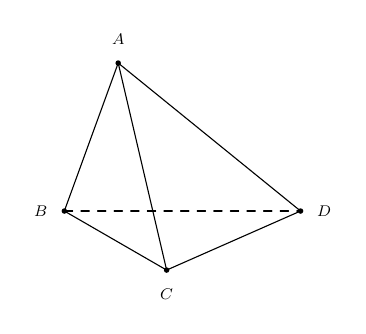
\begin{tikzpicture}[scale=1,font=\footnotesize,line join=round,line cap=round,>=stealth]
					\path (0,0)  coordinate (B)
						(3,0)  coordinate (D)
						(-30:1.5) coordinate (C) 
						(70:2) coordinate  (A);
					\draw (A)--(B)--(C)--(D)--cycle (C)--(A); 
					\draw[dashed] (B)--(D); 
					\foreach \x/\g in  {A/90,B/180,C/-90,D/0}{
						\fill (\x) circle (1pt)+(\g:0.3) node{$\x$}; 
					} 
				\end{tikzpicture}
			 &
			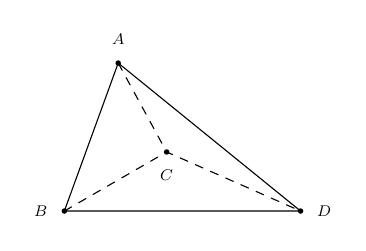
\begin{tikzpicture}[scale=1,font=\footnotesize,line join=round,line cap=round,>=stealth]
					\path (0,0) coordinate  (B)
						(3,0)  coordinate (D)
						 (30:1.5) coordinate (C)
						(70:2)  coordinate (A);
					 \draw (A)--(B)--(D)--cycle;
					\draw[dashed] (B)--(C)--(D) 
						(A)--(C); 
					 \foreach \x/\g in {A/90,B/180,C/-90,D/0}{
						\fill  (\x) circle (1pt)+(\g:0.3) node{$\x$};
					} 
				\end{tikzpicture}
			& 
			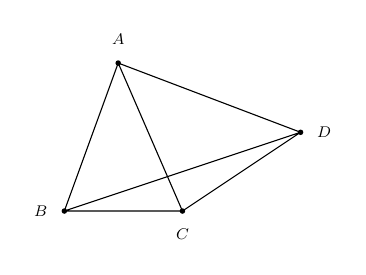
\begin{tikzpicture}[scale=1,font=\footnotesize,line join=round,line cap=round,>=stealth]
					\path (0,0)  coordinate (B)
						(3,1) coordinate (D) 
						(0:1.5) coordinate (C) 
						 (70:2) coordinate (A);
					\draw (A)--(B)--(C)--(D)--cycle (A)--(C) 
						 (B)--(D);
					\foreach \x/\g in  {A/90,B/180,C/-90,D/0}{
						\fill (\x) circle (1pt)+(\g:0.3)  node{$\x$};
					 }
				\end{tikzpicture}
			 &
			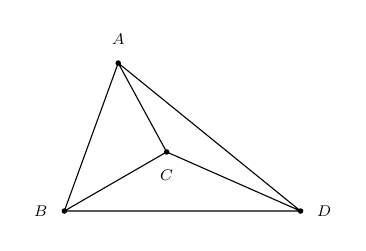
\begin{tikzpicture}[scale=1,font=\footnotesize,line join=round,line cap=round,>=stealth]
					\path  (0,0) coordinate (B)
						 (3,0) coordinate (D)
						 (30:1.5) coordinate (C)
						(70:2) coordinate (A); 
					\draw  (A)--(B)--(D)--cycle (A)--(C)--(D)
						 (C)--(B);
					\foreach \x/\g in {A/90,B/180,C/-90,D/0}{ 
						\fill (\x) circle  (1pt)+(\g:0.3) node{$\x$};
					} 
				\end{tikzpicture}
			\\ 
			Hình $1$ & Hình $2$  & Hình $3$ & Hình $4$
		\end{tabular}
	\end{center}
	\choice 
		{\True Hình $1$, Hình $2$, Hình  $4$}
		{Hình $1$, Hình $2$,  Hình $3$, Hình $4$}
		 {Hình $1$}
		{Hình $1$,  Hình $2$, Hình $3$}
	\loigiai{ 
		Các Hình $1$, Hình $2$,  Hình $4$ biểu diễn một hình tứ diện.\\
		Hình $3$ không phải  là hình biểu diễn của một hình tứ diện vì điểm $AC$ và $BD$ là các nét liền, cắt nhau nên $ABCD$ là tứ giác.
	 }
\end{ex}

% từ: cau-hoi/lop11/1H4_Duong_thang_mat_phang_Quan_he_song_song/1H4-2-1_Cau_hoi_ly_thuyet.tex
\begin{bt}%[1H4H2-1]%[ma:36943946]
% nguon: Archive/2024/TOAN_11_XE/TOAN_11_XE/data4/11C4/BTTN5.tex #722
%[TeX hóa SGK CTST]%[Trúc Danh]
	Trong các mệnh đề sau, mệnh đề nào đúng?
	\begin{enumerate}
		\item Một đường thẳng có thể song song với hình chiếu của nó.
		\item Một đường thẳng có thể trùng với hình chiếu của nó.
		\item Hình chiếu song song của hai đường thẳng chéo nhau có thể song song với nhau.
		\item Hình chiếu song song của hai đường thẳng chéo nhau có thể trùng nhau.
	\end{enumerate}
	\loigiai{
		\begin{enumerate}
			\item Đúng.
			\item Đúng.
			\item Đúng.
			\item Sai, vì hình chiếu song song của hai đường thẳng chéo nhau cắt nhau hoặc song song.
		\end{enumerate}
		
	}
\end{bt}

% từ: cau-hoi/lop11/1H4_Duong_thang_mat_phang_Quan_he_song_song/1H4-3-2_Duong_thang_song_song_voi_mat_phang.tex
\begin{ex}%[1H4H3-2]%[ma:eb967de6]
 Cho lăng trụ tam giác $ ABC.A'B'C'$ có  $ I$, $K$, $G$ lần lượt là trọng tâm các tam giác $ ABC$, $A'B'C'$, $ACC'$. Các mệnh đề sau đúng hay sai?
 \choiceTF 
  {\True$  BB'\parallel \left(ACC'A'\right)$}
  {\True$\left(ABC\right)\parallel  \left(A'B'C'\right)$}
  {$ IG$ cắt $\left(BCC'B'\right)$} 
  {\True$ (IKG)\parallel \left(BCC'B'\right)$} 
 \loigiai{ 
  \begin{center}
   \begin{tikzpicture}[line join = round,line cap = round,font=\footnotesize,>=stealth,scale=1]
      \coordinate (B') at (0,0);
     \coordinate (A') at  (-2,1);
     \coordinate  (C') at (4,1);
     \coordinate (B) at (0,4); 
     \coordinate  (A) at (-2,5);
      \coordinate (C) at (4,5);
     \coordinate  (M) at ($(C)!0.5!(B)$);
     \coordinate (M') at  ($(C')!0.5!(B')$);
     \coordinate (N)  at ($(C)!0.5!(C')$);
     \coordinate (I) at ($(A)!2/3!(M)$); 
     \coordinate (K)  at ($(A')!2/3!(M')$);
     \coordinate (G)  at ($(A)!2/3!(N)$);
     \draw  (A')--(B')--(C')--(C)
       (A)--(B)--(C)--(A)--(A')
       (B)--(B')
      (A)--(M)--(N) 
       (M)--(M');
     \draw[dashed,thin] (A)--(C')--(A') 
      (A)--(N) 
       (I)--(G)
       (A')--(M')
      (I)--(K); 
     \foreach \i/\g in {A'/-90,B'/-90,C'/-90,A/90,B/90,C/90,M/90,N/0,I/90,K/-40,G/-130,M'/-90}{\draw[fill=black](\i)  circle (1pt)
       ($(\i)+(\g:3mm)$) node[scale=1]{$\i$};}
    \end{tikzpicture}
  \end{center}
  \begin{itemchoice}
   \itemch Ta có: $\heva{&BB'\parallel AA'\\&AA'\subset\left(ACC'A'\right)} 
   \Rightarrow  BB'\parallel \left(ACC'A'\right)$.\\
   Vậy mệnh đề $  BB'\parallel \left(ACC'A'\right)$ đúng.
   \itemch Ta có: $\left(ABC\right)\parallel \left(A'B'C'\right)$ (do $\left(ABC\right),\left(A'B'C'\right)$ là hai mặt phẳng chứa hai đáy của lăng trụ nên song song với nhau).\\ 
   Vậy mệnh đề $\left(ABC\right)\parallel \left(A'B'C'\right)$  đúng.
   \itemch Gọi  $ M$, $M'$ lần lượt là trung điểm của $ BC$, $B'C'$.
   Gọi $  N$ là trung điểm của $ CC'$, tam giác $ AMN$ có\\
   $\dfrac{AI}{AM}=\dfrac{AG}{AN}=\dfrac{2}{3}{\rm}$ (tính chất trọng  tâm).\\
   Suy ra $ IG\parallel MN$ mà $ MN\subset\left(BCC'B'\right)$ nên $ IG\parallel \left(BCC'B'\right)$.\hfill  $(1)$\\
   Vậy mệnh đề $ IG$ cắt $\left(BCC'B'\right)$  sai.
   \itemch $ MM'$ là đường  trung bình của hình bình hành $ BCC'B'$ nên\\
    $\heva{&MM'\parallel BB'\\&MM'=BB'}
   \Rightarrow\heva{&MM'\parallel  AA'\\&MM'=AA'}
    \Rightarrow AMM'A'$ là hình bình hành.\\
   Vì $ I$, $K$ theo  thứ tự là trọng tâm các tam giác $ ABC$, $A'B'C'$ nên\\
   $ IM=KM'=\dfrac{1}{3}A'M'=\dfrac{1}{3}AM$, mà $ IM\parallel KM'$ nên $ IKM'M$  là hình bình hành.\\
   Suy ra $ IK\parallel MM',MM'\subset\left(BCC'B'\right)\Rightarrow  IK\parallel \left(BCC'B'\right)$.\hfill $(2)$\\
   Từ $(1)$ và $(2)$ suy ra $ (IKG)\parallel \left(BCC'B'\right)$.  Vậy mệnh đề $ (IKG)\parallel \left(BCC'B'\right)$ đúng.
  \end{itemchoice}
 } 
\end{ex}

% từ: cau-hoi/lop11/1H4_Duong_thang_mat_phang_Quan_he_song_song/1H4-3-2_Duong_thang_song_song_voi_mat_phang.tex
\begin{bt}%[1H4V3-2]%[ma:42245561]
% nguon: Archive/SP_KhoLatex/ID6_old/1-CK1-OT-De-15.tex #3646
%[Dự án đề cuối kỳ 1,2023-2024]%[Lê Hồng Phi]
Cho hình lăng trụ $ABC.A'B'C'$. Gọi $M$, $N$ lần lượt là trọng tâm các tam giác $ABC$, $ACC'$. Chứng minh $MN \parallel \left(ABC'\right)$.
\loigiai
{\immini{Gọi $E$, $F$ lần lượt là trung điểm của $AB$ và $AC'$.
Khi đó $EF$ là đường trung bình của tam giác $ABC'$ nên $EF\parallel BC'$.\hfill $(1)$\\
Theo tính chất của trọng tâm tam giác ta có $\dfrac{CM}{CE}=\dfrac{2}{3}=\dfrac{CN}{CF}$. Suy ra $MN\parallel EF$.\hfill $(2)$\\
Từ $(1)$ và $(2)$ suy ra $MN\parallel BC'$. Mà $MN\not\subset (ABC')$ nên $$MN\parallel (ABC').$$}{\begin{tikzpicture}[scale=1, font=\footnotesize, line join=round, line cap=round,>=stealth]
\path (0,0)coordinate (C) (3.5,0) coordinate (A) (1.3,-1) coordinate (B) (0.5,3.5) coordinate (h);
\foreach \p in {A,B,C} {\draw (\p)--(\p)--+(h) coordinate (\p');}
\path (barycentric cs:A=1,B=1,C=1) coordinate (M) (barycentric cs:A=1,C'=1,C=1) coordinate (N) (barycentric cs:A=1,B=1) coordinate (E) (barycentric cs:A=1,C'=1) coordinate (F);
\draw (A')--(B')--(C')--cycle (A)--(B)--(C) (B)--(C');
\draw[dashed] (C')--(A)--(C)--(E)--(F)--(C) (M)--(N);
\foreach \p/\g in {C/180,B/-90,A/0,C'/180,B'/90,A'/0,M/-60,N/120,E/-60,F/60} \fill[black] (\p) circle(1pt)+(\g:0.3) node{$\p$};
\end{tikzpicture}}
}
\end{bt}

% từ: cau-hoi/lop11/1H4_Duong_thang_mat_phang_Quan_he_song_song/1H4-5-2_Bai_toan_ve_hinh_lang_tru_xien.tex
\begin{ex}%[1H4H5-2]%[ma:85639b23]
  Cho hình lăng trụ $ABC.A'B'C'$.
 \choiceTF 
  {\True  $AA' \parallel CC'$}
  {\True $A'$ hình chiếu của $A$ trên mặt phẳng $(A'B'C')$ qua phép  chiếu song song theo phương $CC'$}
  {\True Gọi $M$ là một điểm trên đoạn thẳng $AB$.  Hình chiếu của $M$ trên mặt phẳng $(A'B'C')$ qua phép chiếu song song theo phương $BB'$ là điểm $M' \in A'B'$}
  {\True Gọi $O$ là tâm của hình bình hành $BCC'B'$. Ảnh của $O$ qua phép chiếu song song theo phương $AA'$ trên mặt phẳng $(A'B'C')$ là trung  điểm của $B'C'$}
 \loigiai{\begin{center}
  \begin{tikzpicture}[line join=round,line cap=round,>=stealth,thick]
    \coordinate (B) at  (0,0.6);
    \coordinate (A) at  (-2,2);
     \coordinate (C) at (3,2);
     \coordinate (A') at (-3,-2);
    \coordinate (B') at  (-1,-3.4);
    \coordinate (C') at  (2,-2);
    \coordinate (M')  at ($(A')!0.5!(B')$);
    \coordinate (M) at  ($(A)!0.5!(B)$);
    \coordinate (I) at ($(C')!0.5!(B')$); 
    \coordinate (O) at  (intersection of B--C' and C--B');
    \draw  (A)--(C)
      (A)--(B)
      (B)--(C)
      (A')--(B')
      (B')--(C')
      (B)--(C')
     (C)--(B') 
     (O)--(I) 
     (A)--(A') 
      (B)--(B')
     (C)--(C') 
     (M)--(M'); 
     \draw[dashed](A')--(C');
    \foreach \i in {A,A'}{\draw (\i) node[scale=0.9,left]{$\i$};} 
    \foreach \i  in {A,B,C,O,I,A',B',C',I,M,M'}{\draw[fill=](\i) circle (1pt);}
    \foreach \i  in {M,B}{\draw (\i) node[scale=0.9,above]{$\i$};}
     \foreach \i in {C,C'}{\draw (\i) node[scale=0.9,right]{$\i$};}
    \foreach \i in {M',B',I}{\draw  (\i) node[scale=0.9,below]{$\i$};}
    \foreach \i in {O}{\draw  (\i) node[scale=0.9,right]{$\i$};}
   \end{tikzpicture}
 \end{center}
 \begin{itemchoice}
  \itemch \textbf{Đúng}. Theo  tính chất hình lăng trụ các mặt bên là hình chữ nhật .\\ Suy ra $AA' \parallel CC'$.
  \itemch \textbf{Đúng}. Vì $AA' \parallel CC'$ và $A'$ thuộc $(A'B'C')$ nên $A'$ là hình chiếu song song của $A$  trên mặt phẳng $(A'B'C')$ theo phương $CC'$.
  \itemch \textbf{Đúng}. Trong mặt phẳng $(ABB'A')$, kẻ đường thẳng $MM' \parallel BB'$ với $M' \in A'B'$. Khi đó $M'$ là  hình chiếu song song của $M$ trên mặt phẳng $(A'B'C')$ theo phương $BB'$.
  \itemch \textbf{Đúng}. Gọi $I$ là trung  điểm của $B'C'$.\\ Vì $OI$ là đường trung bình của tam giác $BB'C'$ nên $OI \parallel BB'\\ \Rightarrow OI \parallel AA'$ mà $I \in (A'B'C')$ nên $I$ là ảnh của $O$ trên mặt phẳng $(A'B'C')$ qua phép chiếu song song phương $AA'$.
 \end{itemchoice}
} 
\end{ex}

% từ: cau-hoi/lop11/1H4_Duong_thang_mat_phang_Quan_he_song_song/1H4-6-3_Xac_dinh_yeu_to_song_song.tex
\begin{ex}%[1H4H6-3]%[ma:272f8e79]
 Cho hình chóp $S.ABCD$ có đáy  $ABCD$ là một tứ giác lồi. Gọi $M$, $N$, $T$ lần lượt là trung điểm của $SA$, $SC$ và $SD$.
  \choiceTF
   {\True$MN\parallel (ABC)$}
  {\True$(MNT)\parallel  (ABCD)$}
  {Gọi $(\alpha)$ là mặt phẳng đi qua $M$ và song song với $(SBD)$. Thiết  diện của hình chóp với $(\alpha)$ là một tứ giác}
  {Gọi $(\beta)$ là mặt phẳng đi qua $N$ và song song với $(\alpha)$. Gọi $I$ và $J$ lần lượt là giao điểm của  $AC$ với mặt phẳng $(\alpha)$ và $(\beta)$. Khi đó $AC=\dfrac{19}{10}IJ$}
 \loigiai{ 
  \begin{center}
   \begin{tikzpicture}[scale=1,font=\footnotesize,line join=round,line cap=round,>=stealth]
     \def\ad{7} 
      \def\ab{3}
      \def\bc{4}
      \def\as{5}
     \def\gocA{50} 
     \def\gocB{120} 
     \coordinate[label=left:$A$] (A) at (0,0); 
     \coordinate[label=below  left:$B$] (B) at (-\gocA:\ab);
     \coordinate[label=below right:$C$] (C)  at ($(B)+(-5:\bc)$);
     \coordinate[label=right:$D$] (D) at  (\ad,0);
     \coordinate[label=above:$S$] (S) at  (60:\as);
     \coordinate[label=left:$M$] (M) at ($(S)!.5!(A)$); 
     \coordinate[label=right:$N$] (N) at ($(S)!.5!(C)$); 
     \coordinate[label=right:$T$]  (T) at ($(S)!.5!(D)$);
     \coordinate[label=below  right:$K$] (K) at ($(A)!.5!(D)$);
     \coordinate[label=below left:$R$]  (R) at ($(A)!.5!(B)$);
     \coordinate[label=below: $P$] (P) at ($(C)!.5!(B)$); 
     \coordinate[label=right:$Q$] (Q) at  ($(C)!.5!(D)$);
     \path[name path=rk] (R)--(K); 
     \path[name path=ac] (A)--(C); 
     \path[name  path=bd] (B)--(D);
      \path[name path=pq] (P)--(Q);
      \path[name intersections={of= rk and ac,by=I}];
     \path[name intersections={of= bd and  ac,by=O}];
     \path[name intersections={of= pq  and ac,by=J}];
     \coordinate[label=below: $J$] (J)  at (J);
     \coordinate[label=below: $I$] (I) at (I); 
     \coordinate[label=below: $O$] (O) at (O); 
     \draw (A)--(B)--(C)--(D)--(S)--cycle  (B)--(S)--(C)
      (N)--(T) 
      (M)--(R) 
       (P)--(N)--(Q);
      \draw[dashed] (C)--(A)--(D)
       (T)--(M)--(N)
      (P)--(Q) 
      (M)--(K)--(R) 
       (D)--(B)--(K);
     \foreach \diem in {A,B,C,D,I,S,M,N,T,O,K,R,P,J,Q} \fill (\diem) circle (1pt); 
    \end{tikzpicture}
  \end{center}
  \begin{itemchoice}
   \itemch Đúng. Xét tam giác $ASC$ có $MN$ là đường trung bình nên $MN\parallel AC$.\\ $MN$ không nằm  trong $(ABCD)$, $AC\subset (ABCD)$ suy ra $MN\parallel (ABCD)$.
   \itemch Đúng. Theo chứng minh trên ta có $MN\parallel  (ABCD)$, tương tự suy ra $MT \parallel (ABCD)$.\\
   Vậy trong mặt phẳng $(MNT)$ có hai đường thẳng cắt nhau $MN$ và $MT$ cùng song song với $(ABCD)$  nên $(MNT)\parallel (ABCD)$.
   \itemch Sai. Gọi $K, R$ lần lượt là trung điểm của $AD$ và $AB$. Do mặt phẳng $(\alpha)$ đi qua $M$  và song song với $(SBD)$ nên giao tuyến của $(\alpha)$ với $(SAB)$ và $(SAD)$ là $MR$ và $MK$.\\
   Từ đó ta có thiết diện của hình chóp với $(\alpha)$ là tam  giác $MRK$.
   \itemch Sai. Tương tự ta có thiết diện của hình chóp với $(\beta)$ là tam  giác $NPQ$.\\
   Gọi $I, O, J$  lần lượt là giao điểm của $AC$ với $RK, BD, PQ$ ta suy ra $I, J$ chính là giao điểm của $AC$ với $(\alpha)$ và $(\beta)$.\\
   Do $RK$ và $PQ$ là các đường trung bình của tam giác $ABD$ và  tam giác $CBD$ nên ta có $I$ là trung điểm của $AO$, $J$ là trung điểm của $CO$.\\
    Suy ra $AX=XO$, $CY=OY$ và ta có $AC=2IJ$.
  \end{itemchoice}
 } 
\end{ex}

% từ: cau-hoi/lop11/1H4_Duong_thang_mat_phang_Quan_he_song_song/1H4-6-3_Xac_dinh_yeu_to_song_song.tex
\begin{ex}%[1H4V6-3]%[ma:450994df]
 Cho hình chóp $S.ABCD$ có đáy  là hình bình hành, các điểm $M, N, E$ lần lượt là trung điểm của các cạnh $SB, SD$ và $CD$.
 \choiceTF 
   {Giao tuyến của mặt phẳng $(SAB)$ và mặt phẳng $(SCD)$ là đường thẳng qua $S$ và song song $BC$}
  {\True $ME \parallel (SAD)$} 
  {Hai mặt phẳng $(MBD)$ và $(MAC)$  cắt nhau theo giao tuyến $ME$}
  {Thiết diện của hình chóp $S.ABCD$ khi cắt bởi mặt phẳng  $(MNE)$ là một tứ giác lồi}
 \loigiai{ 
  \begin{itemchoice}
   \itemch Sai. Vì $AB \parallel CD$ nên giao tuyến của $(SAB)$ và $(SCD)$ là $Sx  \parallel AB \parallel CD$.
   \itemch Đúng. \begin{center}
   \begin{tikzpicture}[scale=1,font=\footnotesize,line join=round,line cap=round,>=stealth]
      \def\bc{4}
     \def\ba{2} 
      \def\h{4}
     \def\gocB{30} 
     \coordinate[label=below left:$B$] (B) at (0,0); 
     \coordinate[label=above left:$A$] (A) at (\gocB:\ba); 
      \coordinate[label=below:$C$] (C) at (\bc,0);
      \coordinate[label=right:$D$] (D) at ($(C)-(B)+(A)$);
      \coordinate[label=above:$S$] (S) at ($(A)+(0:1)+(90:\h)$);
      \coordinate[label=above:$x$] (x) at ($(B)-(A)+(S)$);
     \coordinate[label=left:$F$] (F)  at ($(B)!.5!(A)$);
     \coordinate[label=below  right:$E$] (E) at ($(C)!.5!(D)$);
     \coordinate[label=left:$M$] (M)  at ($(B)!.5!(S)$);
     \draw (B)--(C)--(D)--(S)--cycle  (S)--(C)
       (x)--(S)--($(A)-(B)+(S)$);
     \draw[dashed]  (A)--(D)
      (S)--(A)--(B) 
      (M)--(E)--(F)--(M); 
     \foreach \diem in {A,B,C,D,S,M,E,F} \fill (\diem) circle  (1pt);
    \end{tikzpicture}
  \end{center}
  Từ $E$ kẻ $EF \parallel  AD$. Ta có $(MFE) \parallel (SAD)$ suy ra $ME \parallel (SAD)$.
  \itemch Sai. Gọi $O$  là tâm hình bình hành $ABCD$ suy ra $\heva{&O\in AC\subset(MAC)\\&O\in BD\subset(MBD)}\Rightarrow MO=(MAC)\cap(MBD)$.
  \itemch Sai.  Dựng thiết diện của hình chóp $S.ABCD$ khi cắt bởi mặt phẳng $(MNE)$. \\
  $(MNE) \cap (SCD)=EN$.  \\
  Kẻ $MI \parallel SC$ suy ra $M, N, E,  I$ đồng phẳng. Ta có
  $(MNE) \cap  (SBC)=SI$.\\
  Trong mặt phẳng $(ABCD)$  có $EI \cap AD=L$.\\
  Trong mặt phẳng $(SAD)$, có $LN  \cap SA=P$.\\
  Suy ra $(MNE)  \cap (SAD)=NP$,
   $(MNE) \cap (SAD)=MP$. \\
  Vậy  thiết diện cần tìm là ngũ giác $MIENP$.
 \end{itemchoice}
} 
\end{ex}

% từ: cau-hoi/lop12/2D1_Ung_dung_dao_ham_de_khao_sat_ham_so/2D1-1-1_Xet_tinh_don_dieu_cua_ham_so_cho_boi_cong_thu.tex
\begin{ex}%[2D1N1-1]%[ma:598f9989]
	Giá trị lớn nhất của  hàm số $y=\dfrac{x+1}{x-2}$ trên $\left[-1;0\right]$ là
	\choice 
		{$-\dfrac{1}{2}$} 
		 {$-\dfrac{2}{3}$}
		 {$2$}
		{\True $0$} 
	 \loigiai{
		Hàm số $y=\dfrac{x+1}{x-2}$ xác định và liên tục trên $\left[-1;0\right]$ có 
		$y'=\dfrac{-3}{(x-2)^2}<0, \, \forall x \in \left[-1;0\right] $.  \\
		Suy ra hàm số nghịch biến trên $\left[-1;0\right]$.\\ 
		Do đó $\max \limits_{\left[-1;0\right] } y  = y(-1) = 0$.
	 }
\end{ex}

% từ: cau-hoi/lop12/2D1_Ung_dung_dao_ham_de_khao_sat_ham_so/2D1-1-1_Xet_tinh_don_dieu_cua_ham_so_cho_boi_cong_thu.tex
\begin{ex}%[2D1H1-1]%[ma:d62c841a]
	Cho hàm số $y=f(x)$ có  đạo hàm là $f'(x) = (x-1)^2(3-x)(x^2-x-1)$. Hỏi hàm số $f(x)$ có bao nhiêu cực tiểu?
	\choice 
		{\True  $1$}
		 {$3$}
		{$0$} 
		{$2$} 
	 \loigiai{
		Ta có  $f'(x)= 0 \Leftrightarrow (x-1)^2(3-x)(x^2-x-1)=0 \Leftrightarrow
		 \hoac{&x=1\\&x=3\\&x=\dfrac{1+\sqrt{5}}{2}\\&x=\dfrac{1-\sqrt{5}}{2}.}$\\
		Lập bảng  biến thiên
		\begin{center}
			\begin{tikzpicture}[>=stealth,scale=1]
				\tkzTabInit[lgt=2,espcl=1.6] 
					 {$x$/1,$f^{\prime}
					(x)$/0.8} 
					 {$-\infty$,$x_1$,$1$,$3$,$x_2$,$+\infty$}
				 \tkzTabLine{,-,0,+,0,+,0,-,0,+,}
			\end{tikzpicture}
		\end{center}
		Suy ra hàm số có  một cực tiểu.
	} 
\end{ex}

% từ: cau-hoi/lop12/2D1_Ung_dung_dao_ham_de_khao_sat_ham_so/2D1-1-1_Xet_tinh_don_dieu_cua_ham_so_cho_boi_cong_thu.tex
\begin{bt}%[2D1C1-1]%[ma:71644fd2]
	Gọi $(P)$ là parabol qua $3$ điểm cực trị của đồ thị hàm số $y=\dfrac{1}{4}x^4-mx^2+m^2$.  Tìm tất cả các giá trị thực của tham số $m$ để $(P)$ qua $A(2;24)$.
	\shortans{6} 
	 \loigiai{$y'=x^3-2mx$, $y'=0\Leftrightarrow\hoac{&x=0\\
		 &x^2=2m.}$\\
		Để đồ thị hàm số có ba cực trị thì $m  > 0$.\\
		$y'=0\Leftrightarrow\hoac{ &x=0\Rightarrow y=m^2\\ 
		&x=\pm\sqrt{2m}\Rightarrow  y=0.}$\\
		Vậy ba điểm cực trị của đồ thị hàm số là $A(0;m^2)$, $B(\sqrt{2m};0)$, $C(-\sqrt{2m};0)$.\\ 
		Gọi $(P)\colon y=ax^2+bx+c$ là parabol qua  ba cực trị của đồ thị hàm số.\\
		 $\Rightarrow\heva{&c=m^2\\
		 &2ma+b\sqrt{2m}+c=0\\
		&2ma-b\sqrt{2m}+c=0}\Leftrightarrow\heva{&c=m^2\\ 
		&a=-\dfrac{m}{2}\\ 
		&b=0}\Rightarrow y=-\dfrac{m}{2}x^2+m^2$.\\ 
		Để $(P)$ đi  qua $A(2;24)$ thì $24=-\dfrac{m}{2}\cdot4+m^2\Leftrightarrow m^2-2m-24=0\Leftrightarrow\hoac{&m=6\\
		&m=-4.}$  \\
		Do $m > 0$  nên nhận $m=6$.
	} 
\end{bt}

% từ: cau-hoi/lop12/2D1_Ung_dung_dao_ham_de_khao_sat_ham_so/2D1-1-2_Xet_tinh_don_dieu_dua_vao_bang_bien_thien_do.tex
\begin{ex}%[2D1N1-2]%[ma:0ecf7772]
	\immini{Cho hàm số $ y=f(x)=ax^3+bx^2+cx+d$ có  đồ thị như hình vẽ bên. Hàm số $ y=f(x)$ đồng biến trên khoảng nào?
	\choice 
		 {$(-1;1)$}
		{$(-\infty;-1)$} 
		{$(2;+\infty)$} 
		{\True $(0;1)$}}{\begin{tikzpicture}[line join=round,line cap=round,>=stealth,scale=0.7]
		\tikzset{ethicknode/.style={scale=0.7}} 
		\draw[->] (-1.6,0)--(3.6,0)  node[above left] {$x$};
		\draw[->] (0,-4.6)--(0,1.6) node[below left]  {$y$};
		\draw (0,0) node [above left] {$O$}; 
		 \foreach \x/\nx in {-1/-1,1/1,2/2,3/3}
		\draw[thin] (\x,1pt)--(\x,-1pt) node  [above left] {$\nx$};
		 \foreach \y/\ny in {-2/-2,-4/-4}
		\draw[thin] (1pt,\y)--(-1pt,\y) node  [left] {$\ny$};
		\draw[dashed,thin](1,0)--(1,-2)--(0,-2); 
		 \draw[dashed,thin](3,0)--(3,-4)--(0,-4);
		\begin{scope}
			\clip (-1.5,-4.5) rectangle  (3.5,1.5);
			\draw[samples=200,domain=-1.5:4,smooth,variable=\x] plot  (\x,{-1*((\x)^3)+3*((\x)^2)+0*(\x)+-4});
		\end{scope}
		\fill (1,-2)  circle (1pt)
			(3,-4) circle  (1pt);
	\end{tikzpicture}
		} 
	 \loigiai{
	Quan sát đồ thị, ta thấy  hàm số $ y=f(x)$ đồng biến trên khoảng $(0;1)$.}
\end{ex}

% từ: cau-hoi/lop12/2D1_Ung_dung_dao_ham_de_khao_sat_ham_so/2D1-1-2_Xet_tinh_don_dieu_dua_vao_bang_bien_thien_do.tex
\begin{bt}%[2D1V1-2]%[ma:0444bc19]
	\immini{ 
	Đạo hàm $f'(x)$ của hàm số $f(x)$ là một hàm  số bậc hai và hàm số $y=f'(x)$ có đồ thị bên. Biết rằng hàm số $f(x)$ có giá trị cực đại là $2$ và giá trị cực tiểu là $-2$. Tìm giá trị của $f(2)$.
	 \shortans{18}}
	{\begin{tikzpicture}[line join=round,line cap = round,>=stealth,xscale=1.2,yscale=0.7,font=\footnotesize]
		\foreach  \x/\y/\z/\g in
			 {0/0/O/-55,-2/0/-2/-145}
		 \draw (\x,\y) circle (1pt) coordinate (\z)
			 ($(\z)+(\g:4.5mm)$) node{$\z$};
		\draw[->] (-3.1,0)--(2,0) node[below]{$x$}; 
		\draw[->] (0,-3)--(0,2.3) node[above]{$y$}; 
		\draw[smooth,samples=100,domain=-2.3:0.3] plot  (\x,{3*(\x)^2 +6*\x});
		\draw  (-1.3,2) node{$y=f'(x)$};
	\end{tikzpicture}
	 }
	\loigiai{ 
		Dựa vào đồ thị, ta thấy $f'(x)$ là hàm  số bậc hai có hai nghiệm là $0$ và $-2$\\ nên $f'(x)=ax(x+2)$ (với $a$ là số thực).\\
		Từ đó $\displaystyle f(x)=\int f'(x)\mathrm{\, d}x=a\left(\dfrac{x^3}{3}+x^2\right)+C$ ( với $C$ là hằng số).\\ 
		Từ đồ thị của $f'(x)$, ta  suy ra bảng biến thiên
		\begin{center}
			\begin{tikzpicture}
				\tkzTabInit[nocadre=false,lgt=1.2,espcl=2.5,deltacl=0.7] 
					{$x$ /.6,$f'(x)$ /.6,$f (x)$ /2} 
					{$-\infty$,$-2$,$0$,$+\infty$} 
				\tkzTabLine{,+,$0$,-,$0$,+,} 
				\tkzTabVar{-/$-\infty$,+/$f (-2)$,-/$f  (0)$,+/$+\infty$}
			\end{tikzpicture}
		\end{center}
		Theo đề bài,  ta có $\heva{&f(-2)=2\\&f(0)=-2}\Rightarrow \heva{&C=-2\\& a\left(-\dfrac{8}{3}+4\right)-2=2}\Rightarrow\heva{&C=-2\\&a=3.}$\\
		Vậy $f(x)=x^3+3x^2-2$ và  $f(2)=18$.
	 }
\end{bt}

% từ: cau-hoi/lop12/2D1_Ung_dung_dao_ham_de_khao_sat_ham_so/2D1-1-2_Xet_tinh_don_dieu_dua_vao_bang_bien_thien_do.tex
\begin{bt}%[2D1N1-2]%[ma:73562f32]
% nguon: Archive/2024/TaiLieuGiangDay/1.HamSo/1. K12 - 4in1 - Hamso/ThubaiGoc/Bai1-Dang2.tex #2749
%[SGK-CD]%[BG12new-4in1, Trần Hoà]
	Cho hai hàm số $y=f(x)$ xác định trên $\mathbb{R}$ có đồ thị như hình dưới đây. Tìm các khoảng đồng biến, nghịch biến hàm số.
	\begin{center}
		\begin{tikzpicture}[scale=1, font=\footnotesize, line join=round, line cap=round, >=stealth]
		\draw[gray!50,thin,opacity=.5] (-3,-2) grid (4,4);
		\draw[->] (-2.9,0)--(4.1,0) node[below] {$x$};
		\draw[->] (0,-2.1)--(0,4.1) node[left] {$y$};
		\draw (0,0) node [below left] {$O$};
		\foreach \x/\nx in {-1/-1,1/1,2/2}
		\draw[thin] (\x,1pt)--(\x,-1pt) node [below] {$\nx$};
		\foreach \y/\ny in {1/1,2/2}
		\draw[thin] (1pt,\y)--(-1pt,\y) node [left] {$\ny$};
		\begin{scope}
			\clip (-2.8,-2) rectangle (4,4);
			\draw[samples=200,domain=-2.5:-0.32,smooth,variable=\x] plot (\x,{-1.4*(\x)^2-2.92*(\x)-0.51});
			\draw[samples=200,domain=-0.32:0.68,smooth,variable=\x] plot (\x,{2.9*(\x)^2+0.05*(\x)});
			\draw[samples=200,domain=0.68:1.44,smooth,variable=\x] plot (\x,{-5.06*(\x)^2+10.44*(\x)-3.38});
			\draw[samples=200,domain=1.44:3.5,smooth,variable=\x] plot (\x,{4.34*(\x)^2-16.99*(\x)+16.64});
		\end{scope}
		\draw (3.4,2) node{$y=f(x)$};
		\draw (0,-4) node{\text{\textit{Hình }} $6a$};
	\end{tikzpicture}
	\end{center}
	\loigiai{
	Quan sát đồ thị, ta thấy hàm số $y=f(x)$ đồng biến trên các khoảng $(-\infty;-1)$, $(0;1)$, $(2;+\infty)$; nghịch biến trên các khoảng $(-1;0)$, $(1;2)$. 
	}
\end{bt}

% từ: cau-hoi/lop12/2D1_Ung_dung_dao_ham_de_khao_sat_ham_so/2D1-1-4_Ung_dung_tinh_don_dieu_de_chung_minh_bat_dang.tex
\begin{bt}%[2D1H1-4]%[ma:39227ceb]
% nguon: Archive/2024/TaiLieuGiangDay/1.HamSo/1. K12 - 4in1 - Hamso/ThubaiGoc/Bai1-Dang4.tex #2656
[Mức độ 2]%[Dự án bài giảng new 4in1, Trần Quang Thạnh]
	Giải phương trình $\log_2 \dfrac{(x+1)^2}{2x} +x^2+1>0$.
	\loigiai{
		Điều kiện $x>0$.\\
		Ta thực hiện biến đổi như sau
		$$\log_2(x+1)^2 -\log_2 2x +(x+1)^2-2x>0 \Leftrightarrow \log_2(x+1)^2 +(x+1)^2 >\log_2 2x +2x.$$
		Vì hàm số $f(x)=\log_{2} t$ đồng biến trên khoảng $(0;+\infty)$ nên từ phương trình trên ta được
		$$f\left((x+1)^2\right)>f(2x) \Leftrightarrow (x+1)^2>2x \Leftrightarrow x^2+1 >0.$$
		Kết hợp điều kiện, ta có tập nghiệm bất phương trình là $S=(0;+\infty)$.
	}
\end{bt}

% từ: cau-hoi/lop12/2D1_Ung_dung_dao_ham_de_khao_sat_ham_so/2D1-2-2_Tim_cuc_tri_dua_vao_BBT_do_thi.tex
\begin{ex}%[2D1N2-2]%[ma:1a536494]
	\immini{Cho hàm số $y=f(x)$ có đồ thị như hình bên. Phát biểu nào sau đây là đúng? 
	\choice 
		{$y_{\text{ CT}}=1,y_{\text{  CĐ}}=2$}
		{$y_{\text{  CT}}=2,y_{\text{ CĐ}}=-1$}
		 {$y_{\text{ CT}}=-2,y_{\text{ CĐ}}=2$}
		{\True $y_{\text{  CT}}=2,y_{\text{ CĐ}}=-2$}
		}{\resizebox{!}{5cm}{ 
		\begin{tikzpicture}[scale=0.5,>=stealth,line join=round,line cap=round]
			\draw[->] (-6,0)--(6,0) node[below]{$x$}; 
			\draw[->]  (0,-6)--(0,6) node[left]{$y$};
			\draw[samples=100,domain=-5:-0.175]  plot (\x,{(\x)+1/(\x)});
			\draw[samples=100,domain=0.18:5]  plot (\x,{(\x)+1/(\x)});
			 \draw[samples=100,domain=-5:5] plot (\x,{(\x)});
			\draw (0,0) node[below  right]{$O$};
			 \draw[dashed]
				(-1,0)  node[below left]{$-1$}
				(0,-2)  node[right]{$-2$}
				(0,2) node[above left]{$2$} 
				(1,0)  node[below right]{$1$}
				 (1,0)--(1,2)--(0,2)
				 (-1,0)--(-1,-2)--(0,-2);
			\fill (1,2)  circle (1pt)
				 (-1,-2) circle (1pt)
				(0,0) circle (1pt); 
		\end{tikzpicture}
		 }
		 }
	\loigiai{ 
		Dựa vào đồ thị ta thấy hàm số có $y_{\text{ CT}}=2, y_{\text{ CĐ}}=-2$. 
	} 
\end{ex}

% từ: cau-hoi/lop12/2D1_Ung_dung_dao_ham_de_khao_sat_ham_so/2D1-2-7_Toan_thuc_te_ung_dung_cuc_tri_cua_ham_so.tex
\begin{bt}%[2D1V2-7]%[ma:7b9935f7]
	Một khu vực trồng hoa được xây dựng trong khu du lịch sinh thái. Trong mô hình minh họa (như hình vẽ bên), nó được giới hạn bởi các trục tọa độ và đồ thị $(C)$ của một hàm số bậc ba. Biết rằng đồ thị $(C)$ đi qua các điểm $A(0; 8), B(2; 5,4), K(5; 6,75)$ và $H(8; 0)$. Trong khu du lịch sinh thái  có một con đường chạy dọc theo đường thẳng $d: y=-\dfrac{13}{9} x+\dfrac{169}{9}$. Tìm hoành độ của điểm $M$ thuộc $(C)$ sao cho khoảng cách từ $M$ đến $d$ là nhỏ nhất (làm tròn kết quả đến hàng phần trăm).
	\begin{center}
		\begin{tikzpicture}[line join = round,line cap=round,>=stealth,font=\footnotesize,scale=0.5]
			 \def\f (\x){(-0.1*(\x)^3+1.05*(\x)^2-3*(\x)+8)}
			\draw[->]  (-0.5,0)--(0,0) node[below
				 left]{$O$}--(14,0)
				 node[above]{$x$};
			\draw[->] (0,-0.5)--(0,11) 
				 node[left]{$y$};
			 \fill[pattern=crosshatch dots,smooth] (0,0) --
				plot[domain=0:8] (\x,{\f (\x)}) 
				-- (8,0)  -- cycle;
			\draw[smooth,red,line width=1] 
				 plot[domain=0:8]
				(\x,{\f  (\x)});
			\draw (2,0) node[below]{$2$} 
				 (13,0) node[below]{$13$}
				(8,0) node[below]{$8$} 
				(8,0) node[above right]{$H$} 
				 (0,8) node[right]{$A$}
				 (6,10) node[right]{$d$}
				 (5,0) node[below]{$5$}
				(0,8) node[left]{$8$} 
				(0,6.75)  node[left]{$6,75$}
				 (0,5.4) node[left]{$5,4$};
			\draw[line  width=1pt]((4.6,11)--(13,0);
			\draw[dashed] (5,0)--(5,6.75) node[above]{$K$}--(0,6.75) 
				(2,0)--(2,5.4)  node[above]{$B$}--(0,5.4);
		\end{tikzpicture}
	\end{center}
	 \shortans{6,16}
	 \loigiai{
		Đồ thị $(C)$ của một hàm số  bậc ba có dạng: $f(x)=a x^3+b x^2+c x+d(a \neq 0)$.
		Vì  đồ thị $(C)$ đi qua các điểm $A(0; 8), B(2; 5,4), K(5; 6,75)$ và $H(8; 0)$ nên ta có:
		$\left\{\begin{array}{l}d=8 \\ 8 a+4 b+2 c+d=5,4 \\ 125 a+25 b+5 c+d=6,75 \\ 512 a+64 b+8 c+d=0
	\end{array} \Leftrightarrow\left\{\begin{array}{l}a=-\dfrac{1}{10} \\ b=\dfrac{21}{20} \\ c=-3 \\ d=8
	\end{array}\right.\right.$.
	Suy ra $f(x)=-\dfrac{1}{10} x^3+\dfrac{21}{20} x^2-3 x+8$. 
	Điểm $M$ thuộc $(C)$ sao cho khoảng cách từ $M$ đến $d$ là nhỏ nhất khi và chỉ khi tiếp tuyến của $(C)$ tại $M$  song song với $d\left(x_M>5\right)$.
	 Ta có: $f'(x)=-\dfrac{3}{10} x^2+\dfrac{21}{10} x-3$.
	Đường thẳng $d$  có hệ số góc $k=-\dfrac{13}{9}$.
	Suy ra: $-\dfrac{3}{10} x^2+\dfrac{21}{10} x-3=-\dfrac{13}{9} \Leftrightarrow\left[\begin{array}{l}x=6,16 \\ x=0,84<5
	\end{array}\right.$.
	Do $x_M>5$ nên $x_M=6,16$ thỏa  mãn.
	 }
	\end{bt}

% từ: cau-hoi/lop12/2D1_Ung_dung_dao_ham_de_khao_sat_ham_so/2D1-2-7_Toan_thuc_te_ung_dung_cuc_tri_cua_ham_so.tex
\begin{bt}%[2D1V2-7]%[ma:2acb8871]
	Trong lớp học, màn hình tivi hình chữ nhật có chiều cao $1m$ được đặt ở  độ cao $1.2m$ so với tầm mắt của học sinh (tính từ đầu mép dưới của màn hình). Để nhìn rõ nhất phải xác định vị trí ngồi sao cho góc nhìn lớn nhất ($\widehat{BOC}$ là góc nhìn).
	\begin{center}
		\begin{tikzpicture}[scale=1.2]
			 \path
				(0,0)  coordinate (O)
				(-3,0) coordinate (A) 
				(-3,1.5) coordinate  (B)
				(-3,2.5) coordinate  (C);
			 \draw (O) node[above right]{\text{ \footnotesize Vị trí mắt}}--(B)--node[left]{\text{ \footnotesize Tivi}} node[right]{$ 1 $}
				 (C)--cycle;
			\draw[dashed]  ($(A)-(2,0)$)--($(O)+(2,0)$)
				(A)--node[right]{$ 1,2  $}
				(B); 
			\draw  pic[draw,angle radius=1cm]{angle=C--O--B};
			\draw pic[draw,angle radius=0.3cm]{right angle=O--A--B}; 
			 \foreach \i/\g in {O/-40,B/240,C/120,A/-90}{\fill (\i) circle (1pt) node[shift={(\g:10pt)}]{$\i$};}
		\end{tikzpicture}
	\end{center}
	Nếu xét những học sinh ngồi nhìn thẳng màn hình thì học sinh ngồi bàn thứ mấy nhìn được rõ  nhất, biết bàn đầu tiên cách tivi $1.2m$ và mỗi bàn kế tiếp nhau cách nhau $0.4m$.
	 \shortans{2}
	\loigiai{ 
		Đặt  $OA=x$, ta có $OB=\sqrt{x^2+1.44}$, $OC=\sqrt{x^2+4.84}$\\
		Ta có: $\cos{\widehat{BOC}} = \dfrac{OB^2+OC^2-BC^2}{2. OB.  OC} = \dfrac{x^2+2.64}{\sqrt{x^2+1.44}.\sqrt{x^2+4.84}}$\\
		Đặt $t=x^2, t>0$. Xét  $f(t) = \dfrac{t+2.64}{\sqrt{t+1.44}.\sqrt{t+4.84}} = \dfrac{t+2.64}{\sqrt{t^2+6.28t+6.9696}}$\\
		Ta  có: $f'(t) = \dfrac{0.5t-1.32}{(\sqrt{t^2+6.28t+6.9696})^3}$\\
		Khi  đó: $f'(t)=0 \Leftrightarrow t=2.64$
	} 
\end{bt}

% từ: cau-hoi/lop12/2D1_Ung_dung_dao_ham_de_khao_sat_ham_so/2D1-3-4_Ung_dung_GTNN_GTLN_trong_bai_toan_phuong_trin.tex
\begin{bt}%[2D1H3-4]%[ma:48fa1101]
% nguon: Archive/2024/TaiLieuGiangDay/1.HamSo/1. K12 - 4in1 - Hamso/ThubaiGoc/Bai3-Dang6.tex #2022
[Mức độ 2]%[BG12-4IN1, Nguyễn Khánh Trọng]
	Tìm tất cả giá trị của tham số $m$ để bất phương trình $\mathrm{e}^x\ge m$ có nghiệm $x\in[0;1]$.
	\loigiai{
		Xét hàm số $f(x)=\mathrm{e}^x$ trên đoạn $[0;1]$.\\
		Ta có $f(x)$ luôn đồng biến trên $(0;1)\Rightarrow \max\limits_{[0;1]}f(x)=f(1)=\mathrm{e}$.\\
		Khi đó, bất phương trình $\mathrm{e}^x\ge m$ có nghiệm $x\in[0;1]$ khi và chỉ khi
		$$\max\limits_{[0;1]}f(x)\ge m\Leftrightarrow m\le \mathrm{e}.$$
		Vậy $m\in(-\infty;\mathrm{e}]$.
	}	
\end{bt}

% từ: cau-hoi/lop12/2D1_Ung_dung_dao_ham_de_khao_sat_ham_so/2D1-3-4_Ung_dung_GTNN_GTLN_trong_bai_toan_phuong_trin.tex
\begin{bt}%[2D1H3-4]%[ma:97d0a666]
% nguon: Archive/2024/TaiLieuGiangDay/1.HamSo/1. K12 - 4in1 - Hamso/ThubaiGoc/Bai3-Dang6.tex #2031
[Mức độ 2]%[BG12-4IN1, Nguyễn Khánh Trọng]
	Tìm giá trị của tham số $m$ để  bất phương trình $\dfrac{x^2+3x+3}{x+1}\geq m$ có nghiệm $x\in [0;1]$.
	\dapso{$m\le \dfrac{7}{2}$}
	\loigiai{Để bất phương trình $\dfrac{x^2+3x+3}{x+1}\geq m$ có nghiệm $x\in [0;1]$ tương đương với
		$$\max\limits_{[0;1]}f(x)\ge m\,\, \text{với} \,\, f(x)=\dfrac{x^2+3x+3}{x+1}.$$
		Ta có $f'(x)=\dfrac{x^2+2x}{(x+1)^2}=0\Leftrightarrow x=0$ (nhận) hoặc $x=-2$ (loại).\\
		$f(0)=3$, $f(1)=\dfrac{7}{2}$. \\
		Suy ra $\max\limits_{[0;1]}f(x)=\dfrac{7}{2}$. Do đó $\dfrac{7}{2}\geq m$.
	}
\end{bt}

% từ: cau-hoi/lop12/2D1_Ung_dung_dao_ham_de_khao_sat_ham_so/2D1-5-8_Toan_thuc_te_ung_dung_khao_sat_ham_so.tex
\begin{ex}%[2D1H5-8]%[ma:63edd708]
% nguon: Archive/SP_KhoLatex/SP_Đề Theo Bài-Khối 12/2-OTGK1-De2.tex #4120

Một chất điểm chuyển động theo phương trình li độ $x(t)=-t^3+18t^2+t+3$, trong đó $t$ tính bằng giây và $x$ tính bằng mét. Xét tính đúng sai của các phát biểu sau
\choiceTF
{\True Li độ của chất điểm ở thời điểm $t=4$ giây là $231$ mét}
{\True Vận tốc của chất điểm tại thời điểm $t=5$ giây là $106\, \mathrm{(m/s)}$}
{Gia tốc của chất điểm tại thời điểm $t=10$ giây là $24\, \mathrm{(m/s^2)}$}
{Khi vận tốc của chất điểm đạt giá trị lớn nhất thì li độ của chất điểm là $231\, (m)$}
	\loigiai{
	\begin{itemchoice}
		\itemch Đúng. Li độ của chất điểm ở thời điểm $t=4$ giây là $x(4)=231\, (m)$.
		
		\itemch Đúng. Ta có $v(t)=x'(t)=-3t^2+36t+1$, suy ra vận tốc của chất điểm ở thời điểm $t=5$ giây là $v(5)=106\, \mathrm{(m/s)}$
		
		\itemch Sai. Ta có $a(t)=v'(t)=x''(t)=-6t+36$. Do đó gia tốc tại thời điểm $t=10$ giây là $a(10)=-24\, \mathrm{(m/s^2)}$
		
		\itemch Sai. Ta có $v(t)=x'(t)=-3t^2+36t+1=109-3(t-6)^2\leq 109$. Do đó giá trị lớn nhất của vận tốc là $109\,\mathrm{m/s}$ đạt khi $t=6$ giây.\\
		Lúc đó li độ của chất điểm là $x(6)=441\, \mathrm{(m)}$.
		
\end{itemchoice}					}
\end{ex}

% từ: cau-hoi/lop12/2D4_Nguyen_ham_tich_phan/2D4-1-2_Nguyen_ham_co_ban_da_thuc_phan_thuc.tex
\begin{ex}%[2D4N1-2]%[ma:f261085d]
	Tìm hàm số $y=f(x)$, biết $f'(x)=3\sqrt{x}+\dfrac{2}{\sqrt[3]x}$,  $(x > 0)$ và $f(1)=1$.
	 \choice
		 {\True $f(x)=2x \sqrt{x}+3\sqrt[3]{x^2}-4$}
		{$f(x)=2x \sqrt{x}-3\sqrt[3]{x^2}+2$} 
		 {$f(x)=\sqrt{x}+3\sqrt[3]{x^2}-3$}
		{$f(x)=x \sqrt{x}+3\sqrt[3]x-3$} 
	 \loigiai{
		Xét 
		\begin{eqnarray*}
			\displaystyle\int\left(3\sqrt{x}+\dfrac{2}{\sqrt[3]x}\right)\mathrm{~d} x&= &\displaystyle\int\left(3\sqrt{x}+\dfrac{2}{\sqrt[3]x}\right)\mathrm{~d}  x \\
			&=&  \displaystyle\int\left(3\sqrt{x}+\dfrac{2}{\sqrt[3]x}\right)\mathrm{~d} x+C.
		\end{eqnarray*}
	} 
\end{ex}

% từ: cau-hoi/lop12/2D4_Nguyen_ham_tich_phan/2D4-1-2_Nguyen_ham_co_ban_da_thuc_phan_thuc.tex
\begin{ex}%[2D4H1-2]%[ma:222c157c]
	Giá  trị của $\displaystyle\int_{0}^{2}|x^2-x|\mathrm{\,d}x$ bằng
	\choice 
		{$\dfrac{2}{3}$} 
		{\True $1$} 
		{$\dfrac{1}{3}$} 
		{$2$} 
	\loigiai{ 
		Ta  có: $x^2-x=0 \Leftrightarrow x=0$ hoặc $x=1$.\\
		Do đó,\begin{align*} \displaystyle\int_{0}^{2}|x^2-x|\mathrm{\,d}x&=\displaystyle\int_{0}^{1}|x^2-x|\mathrm{\,d}x+\displaystyle\int_{1}^{2}|x^2-x|\mathrm{\,d}x\\&=\left|\displaystyle\int_{0}^{1}(x^2-x)\mathrm{\,d}x\right|+\left|\displaystyle\int_{1}^{2}(x^2-x)\mathrm{\,d}x\right|\\&=\left|\left(\dfrac{x^3}{3}-\dfrac{x^2}{2}\right)\bigg|_{0}^{1}\right|+\left|\left(\dfrac{x^3}{3}-\dfrac{x^2}{2}\right)\bigg|_{1}^{2}\right|=\left|-\dfrac{1}{6}\right|+\left|\dfrac{5}{6}\right|=1
	\end{align*}
 }
\end{ex}

% từ: cau-hoi/lop12/2D4_Nguyen_ham_tich_phan/2D4-1-6_Toan_thuc_te_ap_dung_nguyen_ham.tex
\begin{bt}%[2D4H1-6]%[ma:afd44e73]
% nguon: Archive/2024/San pham - To Latex Strong - Tex hoa Lop 12 moi - Dot 3 (Chuong 1 + 2 +3 + 4)/Data/Chuong 4/Canh dieu/To 19 - Dot 17 - Chuong 4 - Bai 1 - CD - De 1.tex #3335
%[Tổ 19-Đợt 17-Chương 4-CD-Đề 1]%[Thinh Ngô]%Câu 5
	Một vật chuyển động với gia tốc được cho bởi hàm số $a(t)=-t^2+2 t$ (m/s$^2$). Tại thời điểm $t=0$ vật có vận tốc $36$ m/s. Tính gia tốc của vật tại thời điểm vật dừng lại.
	\shortans{$-24$}
	\loigiai{
	Ta có $\displaystyle\int\limits a(t) \mathrm{\,d}x=\displaystyle\int\limits\left(-t^2+2 t\right) \mathrm{\,d}x=-\dfrac{t^3}{3}+t^2+C$.\\
	Do đó $v(t)=-\dfrac{t^3}{3}+t^2+C$.\\
	Tại thời điểm $t=0$ vật có vận tốc $36 \mathrm{~m} / \mathrm{s}$ cho nên $v(0)=C=36$.\\
	Suy ra $v(t)=-\dfrac{t^3}{3}+t^2+36$.\\
	Thời điểm vật dừng lại $v(t)=-\dfrac{t^3}{3}+t^2+36=0 \Leftrightarrow t=6$.\\
	Khi đó gia tốc của vật là $a(6)=-24$ (m/s$^2$).	
	}
\end{bt}

% từ: cau-hoi/lop12/2D4_Nguyen_ham_tich_phan/2D4-2-6_Toan_thuc_te_ap_dung_nguyen_ham.tex
\begin{bt}%[2D4V2-6]%[ma:1c7cb1c8]
	Ta biết rằng hàm cầu liên quan đến giá $p$ của một sản phẩm với nhu cầu của người tiêu dùng, hàm cung liên quan đến giá $p$ của sản phẩm với mức độ sẵn sàng cung cấp sản phẩm của nhà sản xuất. Điểm cắt  nhau $(x_0;p_0)$ của đồ thị hàm cầu $p=D(x)$ và đồ thị hàm cung $p=S(x)$ được gọi là điểm cân bằng. Các nhà kinh tế học gọi diện tích của hình giới hạn bởi đồ thị hàm cầu, đường ngang $p=p_0$ và đường thẳng $x=0$ là thặng dư tiêu dùng.
	\begin{center}
		\begin{tikzpicture}[scale=0.55,x=1.5cm,>=stealth,line join=round,line cap=round,font=\footnotesize]
				 \def\xmin{-1}
				\def\xmax{5.5} 
				 \def\ymin{-1.5}
				 \def\ymax{8}
				 \def\f{.125*(\x)^2+1}
				 \def\g{3/64*(\x)^2-9/8*(\x)+27/4}
				\fill [pink!50]  (0,1) plot [domain=0:4] (\x,{\f})--(0,3)--cycle;
				\fill  [orange!50] (0,27/4) plot [domain=0:4] (\x,{\g})--(0,3)--cycle;
				 \draw [->] (\xmin,0)--(\xmax,0) node [below,xshift=-3pt] {$x$};
				\draw [->] (0,\ymin)--(0,\ymax) node  [left,yshift=-4pt] {$p$};
				\fill (0,0)  circle (1pt) node [below left] {$O$};
				\draw [smooth,samples=100]  plot [domain=0:\xmax] (\x,{\f}) plot [domain=0:\xmax] (\x,{\g});
				\draw [dash pattern=on 1pt off 2pt] (0,3) node [left] {$p_0$}--(4,3) node [right=5pt] {$(x_0;  p_0)$}--(4,0) node [below] {$x_0$};
				\draw [fill=white] (0,3) circle (1pt) 
					(4,0) circle (1pt) 
					(4,3)  circle (1.5pt);
			\end{tikzpicture}
	\end{center}
	Giả sử hàm cung và hàm cầu của một loại  sản phẩm được mô hình hóa bởi:
	Hàm cầu $p=-0{,}36x+9$ và hàm cung $p=0{,}14x+2$, trong đó $x$ là đơn vị sản phẩm. Tìm thặng dư tiêu dùng cho loại sản  phẩm này (làm tròn đến hàng phần mười).
	 \shortans{35,3}
	\loigiai{ 
		Để  tìm thặng dư tiêu dùng, trước hết ta cần xác định điểm cân bằng của thị trường.\\
		Điểm cân bằng là điểm mà tại  đó hàm cung bằng hàm cầu:
		\allowdisplaybreaks 
		\begin{eqnarray*}
			&&-0{,}36x+9=0{,}14x+2 \\ 
			&\Leftrightarrow&  7=0{,}5x \\
			&\Leftrightarrow& x_0=\dfrac{7}{0{,}5}=14. 
		\end{eqnarray*}
		Vậy,  điểm cân bằng là $(14; 3{,}96)$.\\
		Thặng dư tiêu dùng là 
		 \allowdisplaybreaks
		\begin{eqnarray*}
			S&=&\displaystyle\int_0^{x_0}  \left[D(x)-p_0\right] \mathrm{\,d}x=\displaystyle\int_0^{14} [(-0{,}36x+9)-3{,}96] \mathrm{\,d}x \approx35{,}3.
		\end{eqnarray*}
	 }
\end{bt}

% từ: cau-hoi/lop12/2D4_Nguyen_ham_tich_phan/2D4-2-6_Toan_thuc_te_ap_dung_nguyen_ham.tex
\begin{bt}%[2D4V2-6]%[ma:94173241]
	\immini{Cho ba Parabol $\left(P_1\right) \colon y = x^2$; $\left(P_2\right)\colon y = 2x^2$; $\left(P_3\right) \colon y = kx^2$ với $k > 2$. Gọi $P$ là điểm bất kỳ thuộc parabol $\left(P_2\right)$ và $S_1$, $S_2$ là diện tích các miền phẳng $\left(H_1\right)$, $\left(H_2\right)$ (các miền được gạch chéo trong hình vẽ). Nếu $S_1 = S_2$ thì giá trị của $k = \dfrac{a}{b}$ với $a$, $b \in \mathbb{N}$ và $\dfrac{a}{b}$ là phân số tối giản. Tính $a + b$. 
	 }
	{\begin{tikzpicture}[>=stealth,line join=round,line cap=round,color=blue,font=\footnotesize,scale=1.2]
		\draw[->] (-0.5,0) --  (3,0) node[below] {$x$};
		\draw[->] (0,-0.5)--(0,4) node[right]{$y$}; 
		\draw (0,0) node[below  left]{$O$};
		\draw (1,2) node[above  right]{$P$};
		\fill[pattern = north east lines,pattern color=cyan,smooth] (0,0)  --plot[domain=0:1] (\x,{2*(\x)^2})-- (0.75,2)--plot[domain=0.75:0] (\x,{3.5*(\x)^2})--cycle;
		\fill[pattern =  north west lines,pattern color=red,smooth] (0,0) --plot[domain=0:1] (\x,{(\x)^2})--(1,2)--plot[domain=1:0] (\x,{2*(\x)^2})--cycle;
		\draw[violet,samples=150,smooth,domain=-0:1.9] plot  (\x,{(\x)^2});
		 \draw[violet,samples=150,smooth,domain=-0:1.35] plot (\x,{2*(\x)^2});
		 \draw[violet,samples=150,smooth,domain=-0:1.02] plot (\x,{3.5*(\x)^2});
		 \draw[dashed] (1,0)--(1,2)--(0,2);
		\draw[->] (0.8,0.9)--(1.3,0.6) node[below right]{\scriptsize  $(H_1)$};
		 \draw[->] (0.7,1.3)--(0.3,1.4) node[above]{\scriptsize $(H_2)$};
		\draw (0.9,3.6) node[above]{\scriptsize $(P_3)$}; 
		 \draw (1.45,3.6) node[above]{\scriptsize $(P_2)$};
		\draw  (2.0,3.6) node[above]{\scriptsize $(P_1)$};
	\end{tikzpicture}
	 }
	\shortans{41} 
	\loigiai{ 
		 Gọi $P\left(x_o; y_o\right) \Rightarrow y_o = 2 x_o^2$.\\
		Hình phẳng $(H_1)$ giới hạn bởi $x = 0$; $x = x_o$; $\left(P_1\right) \colon y = x^2$; $\left(P_2\right) \colon y =  2 x^2$.\\
		Suy ra  diện tích hình phẳng $\left(H_1\right)$ là $S_{\left(H_1\right)} = \displaystyle\int_0^{x_o} \left(2x^2 - x^2\right) \mathrm{\,d}x
		 = \dfrac{x_o^2}{3}$.\\
		Hình phẳng $(H_2)$ giới hạn bởi $y = 0$; $y = 2x_o^2$; $\left(P_2\right) \colon y = 2x^2$; $\left(P_3\right) \colon  y = k x^2$.\\
		Suy  ra diện tích hình phẳng $\left(H_2\right)$ là $$S_{\left(H_2\right)} = \displaystyle\int_0^{2x_o^2} \left(\sqrt{\dfrac{y}{2}} - \sqrt{\dfrac{y}{k}}\right) \mathrm{\,d}y
		=  \left(\dfrac{\sqrt{2}}{3}y\sqrt{y} - \dfrac{2}{3\sqrt{k}}y \sqrt{y}\right) \Big|_0 ^{2x_o^2} = \left(\dfrac{\sqrt{2}}{3} - \dfrac{2}{3\sqrt{k}}\right) 2\sqrt{2}x_0^3.$$
		Theo giải  thiết $S_1 = S_2$ nên ta có
		$$\left(\frac{\sqrt{2}}{3}-\frac{2}{3 \sqrt{k}}\right) 2 \sqrt{2} x_o^3 = \frac{x_o^3}{3} \Leftrightarrow 4 - \dfrac{4 \sqrt{2}}{\sqrt{k}} = 1 \Leftrightarrow \sqrt{k} =  \dfrac{4\sqrt{2}}{3} \Leftrightarrow k= \dfrac{32}{9}.$$
		Khi đó $\heva{&a = 32\\&b = 9} \Rightarrow a + b =  41$.
	} 
\end{bt}

% từ: cau-hoi/lop12/2D4_Nguyen_ham_tich_phan/2D4-2-6_Toan_thuc_te_ap_dung_nguyen_ham.tex
\begin{bt}%[2D4V2-6]%[ma:3dd55735]
	\immini{Một quả bóng bầu dục theo quy định được sử dụng trong giải bầu dục quốc gia có kích thước $28$ cm từ đầu  này đến đầu kia và đường kính $17$ cm ở phần dày nhất (quy định có phép thay đổi một chút về các kích thước này) (Nguồn: NFL).\\
	Hình dạng của một quả bóng bầu dục có kích thước nói trên có thể được tạo thành khi quay quanh trục $Ox$ phần diện tích hình phẳng giới hạn bởi đồ thị hàm số $f(x)=ax^2+bx+c$, trục hoành và các đường thẳng $x=-4$; $x=24$, trong đó $x$ tính bằng centimet (cm). Thể tích (đơn vị: cm$^3$, kết quả làm tròn đến hàng đơn vị) của quả bóng bầu dục có kích thước nói trên bằng bao nhiêu?}{\begin{tikzpicture}[scale=1.5]
		 \fill[orange!100!black!100!]
			 (-2,0).. controls (-1.1,1.4) and (1.1,1.4).. (2,0)
			.. controls (1.1,-1.4)  and (-1.1,-1.4).. cycle;
		 \fill[white!95!brown!10]
			(-1.6,0).. controls (-1.8,0.9) and  (-1.55,0.9).. (-1.35,0)
			.. controls (-1.55,-0.9)  and (-1.8,-0.9).. cycle;
		 \fill[white!95!brown!10]
			(1.6,0).. controls (1.8,0.9) and  (1.55,0.9).. (1.35,0)
			.. controls  (1.55,-0.9) and (1.8,-0.9).. cycle;
		\draw[white,line width=1mm,line  cap=round] (-0.9,0) -- (0.9,0);
		\foreach \x in {-0.7,-0.5,-0.3,-0.1,0.1,0.3,0.5,0.7} 
		\draw[white,line width=0.6mm,line cap=round] (\x,-0.18)  -- (\x,0.18);
		\draw[brown!60!black,line width=0.45mm] 
			(-2,0).. controls (-1.1,1.4) and (1.1,1.4).. (2,0) 
			.. controls (1.1,-1.4) and (-1.1,-1.4)..  cycle;
	\end{tikzpicture}
	 }
	\shortans{3390} 
	\loigiai{ 
		\begin{center}
			\begin{tikzpicture}[line join=round,line cap=round,>=stealth,scale=0.6]
					\tikzset{every  node/.style={scale=0.9}}
					 \draw[->] (-6.1,0)--(25.1,0) node[below left] {$x$};
					\draw[->] (0,-2.1)--(0,10.1) node[below  left] {$y$};
					\draw (0,0) node [below  left] {$O$};
					\foreach \x/\nx in {-4/-4,10/10,24/24} 
					\draw[thin]  (\x,1pt)--(\x,-1pt) node [below] {$\nx$};
					\foreach  \y/\ny in {8.5/8.5}
					 \draw[thin] (1pt,\y)--(-1pt,\y) node [left] {$\ny$};
					 \fill[pattern=north east lines,pattern color=black!60]
						plot[domain=-4:24,samples=200] (\x,{-17/392*(\x)^2+85/98*(\x)+204/49}) 
						 -- (24,0) -- (-4,0) -- cycle;
					 \draw[samples=200,domain=-4:24,smooth,variable=\x]
						 plot (\x,{-17/392*(\x)^2+85/98*(\x)+204/49});
					\coordinate (A) at  (10,8.5);
					\draw[dashed] (A)  -- (10,0);
					\draw[dashed] (A) --  (0,8.5);
				\end{tikzpicture}
		\end{center}Ta thấy đồ thị hàm số $f(x)=ax^2+bx+c$ đi qua các điểm $(-4;0)$, $(24;0)$ và $\left(10;\dfrac{17}{2}\right)$ nên ta có
		hệ phương trình 
		\[\heva{&(-4)^2a+(-4)b+c=0\\&24^2a+24b+c=0\\ &10^2a+10b+c=\dfrac{17}{2}}\Rightarrow \heva{&a=-\dfrac{17}{392}  \\&b=\dfrac{85}{98} \\&c=\dfrac{204}{49}.}\]
		Vậy thể tích của quả  bóng bầu dục trên là
	\[V=\pi\displaystyle\int_{-4}^{24} \left(-\dfrac{17}{392}x^2+\dfrac{85}{98}x+\dfrac{204}{49}\right)^2 \mathrm{\,d}x=\dfrac{16\,284}{15}\pi \approx 3\,390\,(\text{cm}^3).\]} 
\end{bt}

% từ: cau-hoi/lop12/2D4_Nguyen_ham_tich_phan/2D4-3-1_Dien_tich_hinh_phang_duoc_gioi_han_boi_cac_do.tex
\begin{ex}%[2D4H3-1]%[ma:8d5691d4]
	Diện tích hình phẳng giới hạn  bởi các đường $y = x^3 - 3x$ và $y = x$ là
	 \choice
		{\True $\displaystyle\int_{-2}^{2} |x^3 -  4x| \mathrm{\,d}x$}
		{$\displaystyle\int_{-2}^{2} |x^3 + 4x|  \mathrm{\,d}x$}
		{$\displaystyle\int_{-2}^{0} |x^3 -  4x| \mathrm{\,d}x$}
		{$\displaystyle\int_{-2}^{0} |x^3 - 4x|  \mathrm{\,d}x$}
	 \loigiai{
		Xét phương trình $x^3 - 3x = x \Leftrightarrow x^3 - 4x = 0 \Leftrightarrow \begin{cases} x = 0 \\ x = \pm 2
	\end{cases}$.\\ Vậy $S = \displaystyle\int_{-2}^{2} |x^3 - 4x| \mathrm{\,d}x$.
 }
\end{ex}

% từ: cau-hoi/lop12/2H2_Toa_do_cua_vec_to_trong_khong_gian/2H2-1-1_Cong_thuc_ly_thuyet.tex
\begin{ex}%[2H2N1-1]%[ma:72193ded]
	Trong không gian $Oxyz$, cho hai điểm $A(x;  y; z)$, $B\left(x'; y'; z'\right)$. Tọa độ của vectơ $\overrightarrow{AB}$~là
	 \choice{$\left(x+x'; y+y'; z+z'\right)$}
		 {$\left(x-x'; y-y'; z-z'\right)$}
		{\True  $\left(x'-x; y'-y; z'-z\right)$}
		{$\left(x x'; y y';  z z'\right)$}
	 \loigiai{
		Ta có  $\overrightarrow{AB}=\left(x'-x; y'-y; z'-z\right)$.
	} 
\end{ex}

% từ: cau-hoi/lop12/2H2_Toa_do_cua_vec_to_trong_khong_gian/2H2-1-1_Cong_thuc_ly_thuyet.tex
\begin{bt}%[2H2H1-1]%[ma:3de4a91b]
% nguon: Archive/2024/0. [LVH] BG - 12 New - 4in1-20240625T224301Z-001/0. [LVH] BG - 12 New - 4in1/data/data_C2/Bai-1-Dang-1-Cauhoilythuyet.tex #1725
[Cùng Khám phá, Mức độ 2]%[BG - 12 New - 4in1,Lam Huy]
    	Cho hình hộp $ABCD.A'B'C'D'$.
	\begin{enumerate}
		\item Trong các véc-tơ khác $\overrightarrow{0}$, có điểm đầu và điểm cuối là các đỉnh của hình hộp, hãy chỉ ra những véc-tơ:
		\begin{itemize}
			\item Cùng phương với véc-tơ $\overrightarrow{AB}$;
			\item Bằng vectơ $\overrightarrow{AB}$;
			\item Ngược hướng với véc-tơ $\overrightarrow{AA'}$.
		\end{itemize}
		\item Tính độ dài của véc-tơ $\overrightarrow{AC'}$ trong trường hợp $ABCD.A'B'C'D'$ là hình hộp đứng, có $AA'=a$, $AB=b$, $BC=c$ và $\widehat{ABC}=120^{\circ}$.
	\end{enumerate}
	\loigiai{
	\begin{enumerate}
		\item Ta có
	\immini{\begin{itemize}
		\item Vectơ khác $\overrightarrow{0}$ và cùng phương với $\overrightarrow{AB}$ là véc-tơ có giá $AB$, $A'B'$, $CD$, $C'D'$. Đó là các véc-tơ $\overrightarrow{BA}$, $\overrightarrow{A'B'}$, $\overrightarrow{B'A'}$, $\overrightarrow{CD}$, $\overrightarrow{DC}$, $\overrightarrow{C'D'}$, $\overrightarrow{D'C'}$;
		\item Các véc-tơ bằng $\overrightarrow{AB}$ là $\overrightarrow{A'B'}$, $\overrightarrow{DC}$, $\overrightarrow{D'C'}$ (các véc-tơ này cùng hướng và cùng độ dài với $\overrightarrow{AB}$).
		\item Trong những véc-tơ khác $\overrightarrow{0}$ và cùng phương với $\overrightarrow{AA'}$, có bốn vectơ $\overrightarrow{A'A}$, $\overrightarrow{B'B}$, $\overrightarrow{C'C}$, $\overrightarrow{D'D}$ ngược hướng với $\overrightarrow{AA'}$;
	\end{itemize}}{\begin{tikzpicture}[scale=1, font=\footnotesize, line join=round, line cap=round, >=stealth]
		\def\bc{4} % cạnh BC
		\def\ba{2} % cạnh BA
		\def\h{4} % đường cao
		\def\gocB{35} % góc B của đáy
		\coordinate[label=below left:$B$] (B) at (0,0);
		\coordinate[label=above left:$A$] (A) at (\gocB:\ba);
		\coordinate[label=below:$C$] (C) at (\bc,0);
		\coordinate[label=right:$D$] (D) at ($(C)-(B)+(A)$);
		\coordinate[label=above left:$A'$] (A') at ($(A)+(90:\h)$);
		\coordinate[label=left:$B'$] (B') at ($(B)-(A)+(A')$);
		\coordinate[label=below right:$C'$] (C') at ($(C)-(A)+(A')$);
		\coordinate[label=right:$D'$] (D') at ($(D)-(A)+(A')$);
		\draw (B')--(B)--(C)--(D)--(D')--(A')--(B')--(C')--(D') (C)--(C');
		\draw[dashed] (A')--(A)--(D) (A)--(B) (A)--(C) (A)--(C');
		\foreach \diem in {A,B,C,D,A',B',C',D'}	\fill (\diem)circle(1.5pt);
	\end{tikzpicture}}
	\item Xét tam giác $ABC$ ta có  $AC=\sqrt{AB^2+BC^2-2AB\cdot BC\cdot \cos \widehat{ABC}}=\sqrt{b^2+c^2+bc}$. \\
	Từ giả thiết, ta suy ra tam giác $ACC'$ vuông tại $C$. Từ đó ta có:
	$$
	AC'=\sqrt{CC'^2+AC^2}=\sqrt{AA'^2+AC^2}=\sqrt{a^2+b^2+c^2+bc}
	$$
	Vậy độ dài của $\overrightarrow{AC'}$ là $\sqrt{a^2+b^2+c^2+bc}$.
	\end{enumerate}
	}
\end{bt}

% từ: cau-hoi/lop8/8D2_Chuong_II_Hang_dang_thuc_dang_nho_va_ung/8D2-7-3_Tinh_nhanh_rut_gon_bieu_thuc.tex
\begin{bt}%[8D2H7-3]%[ma:430fc03b]
	Tính nhanh giá trị của biểu thức $D = 103^3 - 9 \cdot 103^2 + 27 \cdot 103 - 27$.
	\loigiai{
		Ta biến đổi biểu thức $D$ về dạng lập phương của một hiệu:
		\begin{align*} 
			D &= 103^3 - 3 \cdot 103^2 \cdot 3 + 3 \cdot 103 \cdot 3^2 - 3^3 \\
			&= (103-3)^3 \\
			&= 100^3 \\
			&= 1\,000\,000.
		\end{align*}
	}
\end{bt}

% từ: cau-hoi/lop8/8D2_Chuong_II_Hang_dang_thuc_dang_nho_va_ung/8D2-8-1_Khai_trien_viet_duoi_dang_tich.tex
\begin{bt}%[8D2H8-1]%[ma:b95fa86c]
	Rút gọn biểu thức $A = (x + 2)(x^2 - 2x + 4) - (x - 1)(x^2 + x + 1)$ rồi chứng tỏ giá trị của $A$ không phụ thuộc vào $x$.
	\loigiai{
		Áp dụng hằng đẳng thức tổng hai lập phương và hiệu hai lập phương: \\
$(x + 2)(x^2 - 2x + 4) = x^3 + 2^3 = x^3 + 8$. \\
$(x - 1)(x^2 + x + 1) = x^3 - 1^3 = x^3 - 1$. \\
Suy ra $A = (x^3 + 8) - (x^3 - 1) = x^3 + 8 - x^3 + 1 = 9$. \\
Vậy giá trị của $A$ luôn bằng $9$, không phụ thuộc vào biến $x$.
	}
\end{bt}

% từ: cau-hoi/lop9/9D1_Chuong_I_Phuong_trinh_va_he_hai_phuong_t/9D1-3-4_Toan_thuc_te_hoa_hoc_vat_li_kinh_te.tex
\begin{bt}%[9D1H3-4]%[ma:a823daad]
% nguon: Tuyển tập đề tham khảo môn Toán Tuyển sinh 10 năm học 2025-2026 TP.HCM – Đề tham khảo Huyện Bình Chánh (Đề 2) – Bài 3
Một bức tường hình thang vuông có chiều cao là $h\text{ (m)}$, đáy bé là $4x\text{ (m)}$ và đáy lớn là $8x\text{ (m)}$. Trên bức tường đó người ta thiết kế một cửa sổ hình chữ nhật có chiều rộng là $2x\text{ (m)}$ và chiều cao là $1\text{ m}$.
\begin{enumerate}[a)]
	\item Viết biểu thức biểu thị diện tích bức tường theo $x$ và $h$ (không tính phần cửa sổ).
	\item Tính diện tích của bức tường khi biết $x = 3\text{ m}$ và $h = 4\text{ m}$.
\end{enumerate}
\loigiai{
\begin{enumerate}[a)]
	\item Diện tích của toàn bộ bức tường hình thang vuông ban đầu là:
	$$ S_{\text{thang}} = \dfrac{(4x + 8x) \cdot h}{2} = \dfrac{12x \cdot h}{2} = 6xh\text{ (m}^2\text{)}. $$
	Diện tích của cửa sổ hình chữ nhật là:
	$$ S_{\text{cửa sổ}} = 2x \cdot 1 = 2x\text{ (m}^2\text{)}. $$
	Biểu thức diện tích phần tường còn lại (không tính cửa sổ) là:
	$$ S = 6xh - 2x\text{ (m}^2\text{)}. $$
	\item Thay $x = 3\text{ m}$ và $h = 4\text{ m}$ vào biểu thức diện tích, ta được:
	$$ S = 6 \cdot 3 \cdot 4 - 2 \cdot 3 = 72 - 6 = 66\text{ (m}^2\text{)}. $$
	Vậy diện tích bức tường là $66\text{ m}^2$.
\end{enumerate}
}
\end{bt}

% từ: cau-hoi/lop9/9D1_Chuong_I_Phuong_trinh_va_he_hai_phuong_t/9D1-3-4_Toan_thuc_te_hoa_hoc_vat_li_kinh_te.tex
\begin{bt}%[9D1H3-4]%[ma:abdc11bf]
% nguon: Đề tham khảo Tuyển sinh 10 năm học 2026-2027 Sở GD&ĐT TP.HCM - Cụm 12 Đề 3 (Đề số 36)
Bác Nam có một mảnh vườn hình chữ nhật. Bác chia mảnh vườn này ra làm hai khu đất hình chữ nhật: khu thứ nhất dùng để trồng cỏ, khu thứ hai dùng để trồng hoa (với chiều rộng cả vườn là $y + 1$ (m), chiều dài cả vườn là $2y + 12$ (m) và khu trồng hoa có một kích thước là $2x$ (m)).
\begin{enumerate}[a)]
	\item Biểu diễn diện tích khu đất dùng để trồng hoa và diện tích khu đất dùng để trồng cỏ theo $x, y$.
	\item Tính diện tích toàn bộ mảnh vườn hình chữ nhật của bác Nam với $x = 4$ và $y = 4$.
\end{enumerate}
\loigiai{
\begin{enumerate}[a)]
	\item Khu đất trồng hoa hình chữ nhật có kích thước hai cạnh là $2x$ (m) và $y + 1$ (m).
	Do đó diện tích khu đất dùng để trồng hoa là:
	$$S_{\text{hoa}} = 2x(y + 1)\text{ (m}^2\text{)}.$$
	Khu đất trồng cỏ có chiều rộng là $y + 1$ (m) và chiều dài là:
	$$(2y + 12) - 2x\text{ (m)}.$$
	Do đó diện tích khu đất dùng để trồng cỏ là:
	$$S_{\text{cỏ}} = (2y + 12 - 2x)(y + 1)\text{ (m}^2\text{)}.$$
	\item Với $x = 4$ và $y = 4$, kích thước của mảnh vườn hình chữ nhật là:
	\begin{itemize}
		\item Chiều dài: $2y + 12 = 2 \cdot 4 + 12 = 20\text{ (m)}$.
		\item Chiều rộng: $y + 1 = 4 + 1 = 5\text{ (m)}$.
	\end{itemize}
	Diện tích toàn bộ mảnh vườn hình chữ nhật là:
	$$S = 20 \cdot 5 = 100\text{ (m}^2\text{)}.$$
\end{enumerate}
}
\end{bt}
